\documentclass[11pt,a4paper]{article}
%\usepackage[utf8]{inputenc}
\usepackage[T1]{fontenc}
\usepackage{lmodern}
\renewcommand{\familydefault}{\sfdefault}

\renewcommand{\rmdefault}{\sfdefault} % change math font
\usepackage{mathastext} % change math font

%\usepackage{textgreek}
%\renewcommand{\alpha}{\text{\textalpha}}
%\renewcommand{\beta}{\text{\textbeta}}

\usepackage[margin=2cm]{geometry}
\usepackage{authblk}
\usepackage{titlesec}
\usepackage{amsmath}
\usepackage{dsfont}
\usepackage{multirow}
\usepackage{booktabs}
\usepackage{enumitem}
\usepackage{comment}
\usepackage{threeparttable}
\usepackage{lscape}
\usepackage[table]{xcolor}
\usepackage{graphicx}
\usepackage{float}
\usepackage[labelfont=bf]{caption}
\usepackage[justification=justified,singlelinecheck=false, subrefformat=parens]{subcaption}
\usepackage[acronym]{glossaries}
\usepackage[square,sort,comma,numbers]{natbib}
\usepackage{annotate-equations}
\usepackage[colorlinks=true,linkcolor=black,urlcolor=black,citecolor=black]{hyperref}
\urlstyle{same}

\makeglossaries
\newacronym{cgm}{CGM}{continuous glucose monitoring}
\newacronym{dst}{DST}{daylight saving time}
\newacronym{utc}{UTC}{coordinated universal time}
\newacronym{ftp}{FTP}{functional threshold power}
\newacronym{lthr}{LTHR}{lactate threshold heart rate}
\newacronym{heartrate}{HR}{heart rate}
\newacronym{ci}{CI}{confidence interval}
\newacronym{or}{OR}{odds ratio}
\newacronym{iqr}{IQR}{interquartile range}
\newacronym{kde}{KDE}{kernel density estimation}
%\newacronym{power}{P}{power}

\newcommand\TODO[1]{\textcolor{red}{#1}}
%\newcommand\OR[4]{\gls{or} #1 [#2--#3]}
\newcommand\pval{\textit{p}}
%\glsdisablehyper
\newcommand\subrefb[1]{\textbf{\subref{#1}}}

\titleformat{\subsubsection}[runin]{\normalsize\bfseries}{\thesubsection}{5pt}{}%[\mbox{  }]
%\titleformat{\subsubsection}[runin]{\normalfont\sffamily\bfseries}{}{0em}{}[ --- ]

\newcommand{\hl}[0]{\cellcolor{red!15}}
\newcommand{\ml}[0]{\cellcolor{red!15}}
\newcommand{\bl}[0]{\cellcolor{red!30}}
\newcommand{\si}[0]{}
\newcommand{\nl}[0]{\textcolor{white}{<}}

\title{\textbf{Supplemental Material} \\\vspace{5mm}
Glycemic Control of Male Professional Athletes With Type 1 Diabetes Over an Entire Competitive Season: A Retrospective Observational Analysis}

\author[1]{Eva van Weenen, MSc}
\author[2]{Nicolas Banholzer, PhD}
\author[1]{Simon Föll, MSc}
\author[3,4]{Thomas Züger, MD}
\author[3,5]{Federico Y. Fontana, PhD}
\author[5]{Kristina Skroce, MSc}
\author[5]{Charlotte Hayes, MMSc}
\author[6]{Mathias Kraus, PhD}
\author[7]{Stefan Feuerriegel, PhD}
\author[8]{Felix Wortmann, PhD*}
\author[5]{Sam N. Scott, PhD*}
\author[3]{Christoph Stettler, MD\thanks{Joint last author}}

\affil[1]{Department of Management, Technology and Economics, ETH Zurich, Zurich, Switzerland}
\affil[2]{Institute of Social and Preventive Medicine, University of Bern, Bern, Switzerland}
\affil[3]{Department of Diabetes, Endocrinology, Nutritional Medicine and Metabolism, Bern University Hospital, University of Bern, Bern, Switzerland}
\affil[4]{Department of Endocrinology and Metabolic Diseases, Kantonsspital Olten, Olten, Switzerland}
\affil[5]{Team Novo Nordisk Professional Cycling Team, Atlanta, USA}
\affil[6]{School of Business, Economics and Society, Friedrich-Alexander University Erlangen-Nürnberg, Germany}
\affil[7]{Institute of AI in Management, LMU Munich, Munich, Germany}
\affil[8]{Institute of Technology Management, University of St. Gallen, St. Gallen, Switzerland}

\begin{document}
\maketitle
\setcounter{secnumdepth}{1}
\setcounter{tocdepth}{5}
\renewcommand{\thesection}{\Alph{section}} 
%\renewcommand{\thesubsection}{\arabic{subsection}}

\newpage
\tableofcontents
\newpage
\listoffigures
\listoftables
%\printglossary[type=\acronymtype]

\newpage
\section{Data}
\subsection{Study period}
\subsubsection{Definition of study period}
The study period was defined to be between Oct 2018 and Oct 2019, corresponding to a competitive season in road cycling. Each study participant had an individual start and end of the competitive season, that deviated slightly form the start and end of the study period. Hence, the median season length across participants was 340.0 [interquartile range 314.5--343.5] days. 

\subsubsection{Explanatory statement on study period definition}
The study period was limited to the 2019 competitive season to maximize the number of eligible study participants, and to eliminate potential confounding from the COVID-19 pandemic.

\subsection{Participant eligibility and exclusion of data}
\subsubsection{Patient inclusion criteria}
Individuals were eligible for participation of the study if they
\begin{itemize}[itemsep=0pt, parsep=0pt]
    \item were a Team Novo Nordisk professional road cyclist during the study period;
    \item provided informed consent for the study period; and
    \item had at least 14 days of \gls{cgm} recordings during the study period,
\end{itemize}
where a day was defined to be between 06:00h and 06:00h the next day and a day was only included if the availability of \gls{cgm} data for that day was above 70\%\footnote{The Dexcom G6 collects data at a 5-minute interval. CGM data availability for a day was therefore calculated as the number of measurements for a day divided by the possible number of measurements for a day, i.e., 288}. 

\subsubsection{Justification of $\geq 70\%$ \gls{cgm} availability criteria}
The requirement of $\geq 70\%$ \gls{cgm} availability for an individual day was based upon the \gls{cgm} consensus statement of \citet{29162583}. Figure~\ref{fig:cgm_availability_days} shows the distribution of \gls{cgm} availability for individual days. The area under the distribution left of the red dashed line indicates the percentage of days that will be excluded when implementing this requirement, i.e., 30.5\% of days are excluded. Figure~\ref{fig:cgm_availability_values} shows the distribution of \gls{cgm} availability for individual measurements within a day, i.e., when assigning an availability value to each \gls{cgm} measurement within a day. Here, the area under the distribution left of the red dashed line thus indicates the percentage of \gls{cgm} measurements that will be excluded when implementing this requirement, i.e., 8.5\% of \gls{cgm} measurements are excluded. 

\begin{figure}[h]
    \centering
    \caption[Distribution of CGM availability]{Distribution of CGM availability fitted with \gls{kde}. The 70\% \gls{cgm} availability requirement is demonstrated with a red dashed line. \subrefb{fig:cgm_availability_days} \gls{cgm} availability for individual days. \subrefb{fig:cgm_availability_values} \gls{cgm} availability for individual measurements, i.e., when you assign an availability value to all CGM measurements within a day.}
    \label{fig:cgm_availability}
    \begin{subfigure}[b]{.45\textwidth}
        \centering
        %\caption{\gls{cgm} availability for individual days}
        \caption{}
        \label{fig:cgm_availability_days}
        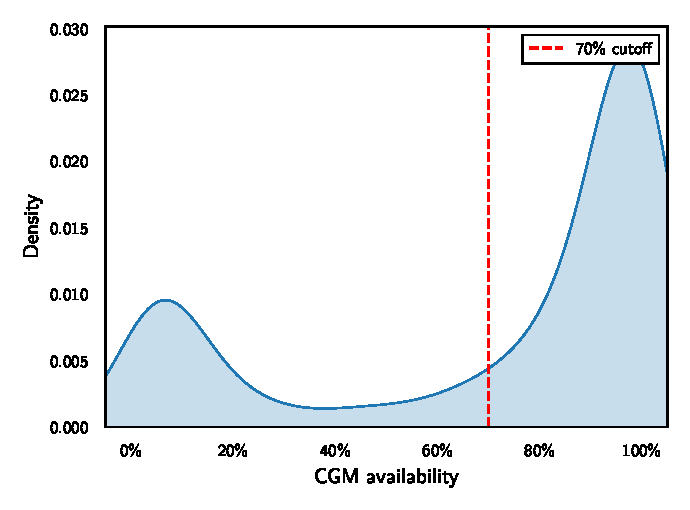
\includegraphics[width=\textwidth]{figure/completeness_cutoff_pdf.pdf}
    \end{subfigure}\hfill
    \begin{subfigure}[b]{.45\textwidth}
        \centering
        %\caption{\gls{cgm} availability for individual measurements, i.e., when you assign an availability value to all CGM measurements within a day}
        \caption{}
        \label{fig:cgm_availability_values}
        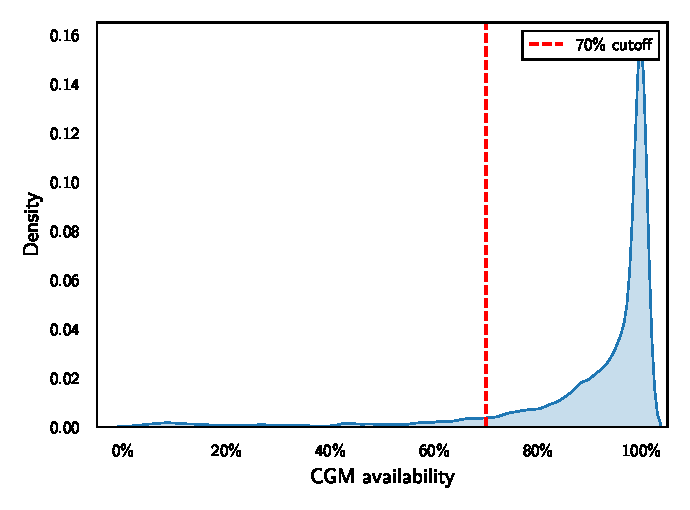
\includegraphics[width=\textwidth]{figure/completeness_cutoff_values_pdf.pdf}
    \end{subfigure}
\end{figure}

\subsubsection{CONSORT flow diagram}
Further details on patient eligibility and exclusion criteria are shown in Figure~\ref{fig:consort}. A total of $n=12$ individuals were included in this study. For the analysis of glycemia, a total of 2,115 days were included. For the analysis on the associations of exercise with dysglycemia, we required additional availability of exercise data during a day. Hence, for this analysis, a total of 1,789 days were used.

\begin{figure}[h!]
    \vspace{2cm}
    \centering
    \caption[CONSORT flow diagram]{CONSORT flow diagram for participant eligibility and data selection.}
    \label{fig:consort}
    \includegraphics[width=\textwidth, trim=1.9cm 0cm 1.8cm 0cm, clip]{figure/CONSORT_v4.pdf}
\end{figure}

\newpage

\subsection{Data collection and processing}
Prior to analysis, careful processing of sensor data was performed to obtain a clean dataset. Here, we describe the steps taken to collect and clean the data. All data were collected and processed in Python version 3.7.5 \cite{python}. For brevity, the description below is a reduced version of the data processing, and does not include include rudimentary cleaning steps, common for any type of data set (e.g., removing zero or erroneous values from columns, removing duplicate rows, etc.). For a full description, we refer to the Python code, which we made publicly available via \TODO{githublink}.

\begin{enumerate}[label=\textbf{\arabic*}.]
\item \textbf{Data collection}
Cycling data were downloaded from the TrainingPeaks platform\footnote{\url{https://www.trainingpeaks.com/}} for all eligible participants for the defined study period. \Gls{cgm} data were downloaded from Dexcom Clarity\footnote{\url{https://clarity.dexcom.eu/}}.

\item \textbf{File format conversion} 
Downloaded exercise files were of the format ANT/Garmin \texttt{.FIT} and were converted to \texttt{.csv} using fitparse \cite{fitparse} version 1.2.0 in Python. 

\item \textbf{Timezone extraction}
GPS latitude and longitude in the exercise files were used to obtain timezone information for a particular day, using geopy version 2.1.0 \cite{geopy} in Python with OpenStreetMap Nominatim\footnote{\url{https://nominatim.org/}}.

\item \textbf{Initial cleaning} 
\Gls{cgm} data was initially cleaned by replacing \textit{high} with 400 mg/dL and \textit{low} with 40 mg/dL, corresponding to the glucose measurement range of the Dexcom G6 \gls{cgm} device. Additionally, all glucose concentrations were converted from the units mmol/L to mg/dL with a conversion factor of 18. 

\item \textbf{Timestamp corrections in \gls{cgm} data} 
Data from the Dexcom G6 \gls{cgm} devices consists fundamentally of a timestamp (i.e., in the format \textit{yyyy-MM-dd HH:mm:ss}) with a glucose value attributed to it. This timestamp in the data originates from the receiving device and corresponds to the moment in time when the receiving device receives the signal that is transmitted from the \gls{cgm} device. The timestamp was recorded in the local timezone of the receiver. Information about the timezone itself was not available in the data. 

Due to frequent travelling as well as occasional \gls{dst}, participants had to frequently adjust the timestamps on their receiving device. Some participants had to make manual adjustments, when their receiver did not have an Internet connection. This introduced human errors when, for instance, the month and day of the month were reversely entered by the participant. Moreover, as data for this study was collected retrospectively, without further instructions on this issue to participants during the study period, participants modified timezone setup of the receiver between zero and three weeks after travelling. The change in timezone setup was thus frequently delayed compared to the actual change. 

When the time setup in the receiving device was incorrect, incorrect timestamps were attributed to glucose measurements in the \gls{cgm} data. It is relevant for our analysis that the timestamps in the \gls{cgm} data are correct, such that we can correctly assign \textit{wake} and \textit{sleep} labels to the timestamps. To correct for this issue, we leveraged the intrinsic time of the transmitter, corresponding to the lifetime (internal clock) of the transmitter in seconds at the time of glucose measurement, as described in the following steps below:
\begin{enumerate}
    \item We manually corrected for any incorrect date setup (e.g., when the month and day were unintentionally switched around by the participant), leveraging the transmitter's intrinsic timestamps.
    \item During the transition between two transmitters, it happened occasionally that glucose measurements had been incorrectly attributed to the previous or subsequent transmitter. Using the transmitter's intrinsic time, we manually modified the incorrect transmitter assignments.
    \item To obtain the correct order in which the \gls{cgm} measurements took place, we sorted the \gls{cgm} data for a participant by chronology of transmitters and the transmitter's intrinsic timestamp.\label{it:sort}
    \item The first step of the timestamp correction was the transformation of incorrect receiver timestamps to correct timestamps in \gls{utc} through identification of (manual) timezone changes in the \gls{cgm} data. Given the correct sorting of the \gls{cgm} data, a change in timezone can be identified in the data as follows. When a participant shifted the time of his receiver forward in time, there will be a \textit{gap} in the sequence of local timestamps at that time. For instance, if a participant travelled at 9am from UTC+01 to UTC+02 and shifted the time of his receiver as such, there will be a gap of at least one hour between 9am and 10am in the sequence of local timestamps. Conversely, when a participant shifted the time of his receiver backwards in time, there will be an \textit{overlap} in the sequence of local timestamps at that time. For instance, if a participant travelled at 9\,am from UTC+01 to UTC+00 and shifted the time of his receiver as such, there will be an overlap of at most one hour between 8\,am and 9\,am in the sequence of local timestamps (see Figure~\ref{fig:gaps-overlaps} for an illustration). 
    
    \begin{figure}[h!]
        \centering
        \caption{Gaps and overlaps in the \gls{cgm} data due to travelling.}
        \label{fig:gaps-overlaps}
        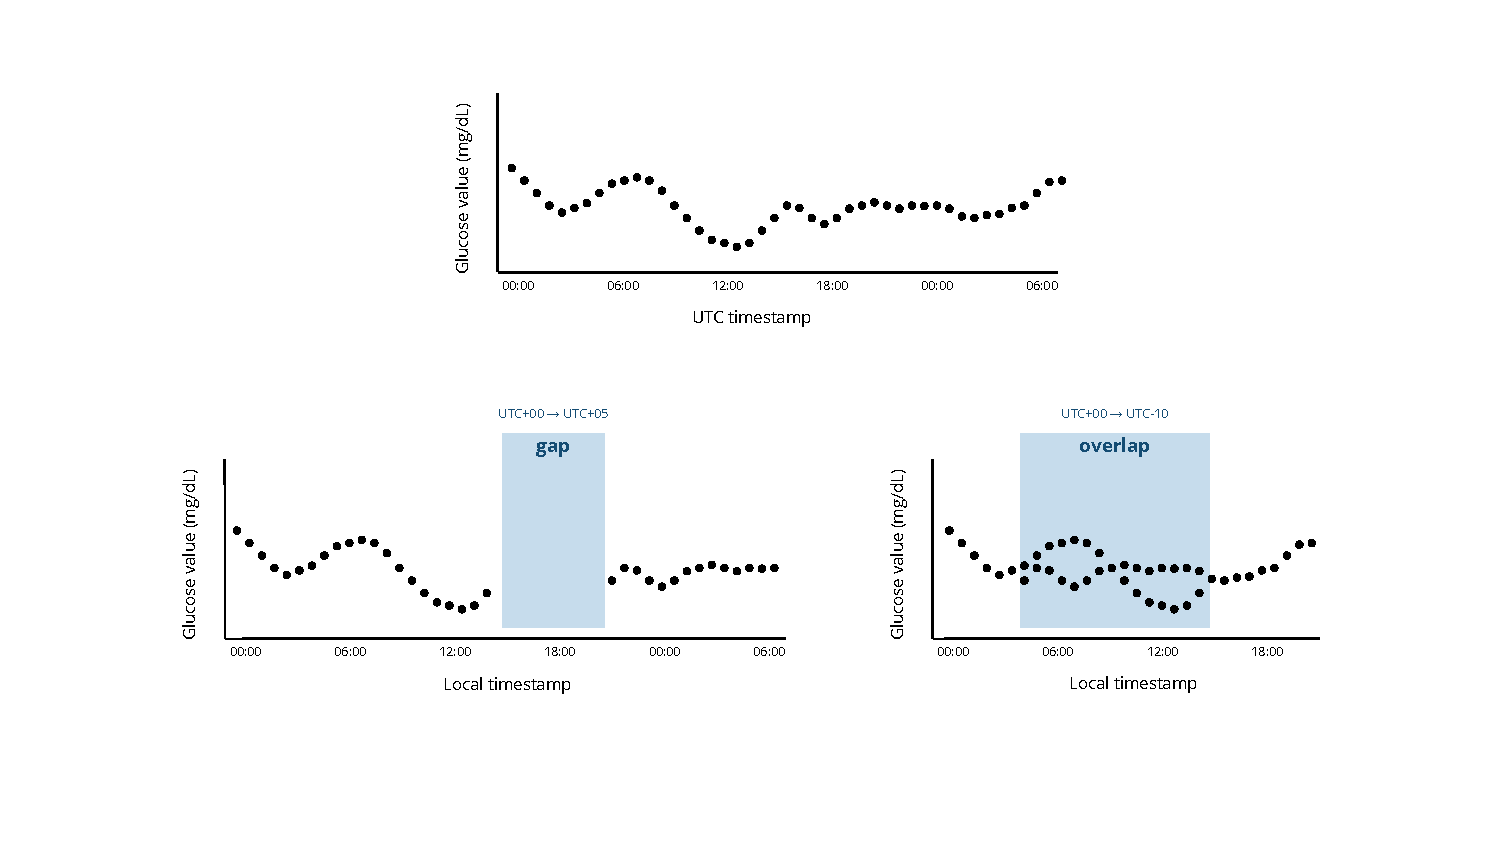
\includegraphics[width=.8\textwidth, trim=3cm 2.5cm 3cm 1.5cm, clip]{figure/gaps_overlaps.pdf}
    \end{figure}
    
    The above transformation is further complicated by censoring, i.e., when \gls{cgm} data has not been recorded for a period of time. Hence, we leveraged the transmitter's intrinsic time to correct for these issues. To identify a change in the time setup of the receiver, we used the following equation:
    \begin{equation}
        Z^{\text{receiver}}_{i} - Z^{\text{receiver}}_{i-1} = \left(T^{\text{receiver}}_{i} - T^{\text{receiver}}_{i-1}\right) - \left(T^{\text{transmitter}}_{i} - T^{\text{transmitter}}_{i-1}\right),
    \end{equation}
    where $i$ is in the index of the data sequence, sorted as described in step (c), $T^{\text{receiver}}_{i}$ is the local timestamp of the receiver at index $i$, $T^{\text{transmitter}}_{i}$ is the transmitter's intrinsic time at index $i$, and $Z^{\text{receiver}}_{i}$ is the timezone of the receiver at index $i$. Hence, the change in the timezone of the receiving device should only be non-zero if there is a non-zero difference in time between two subsequent timestamps of the receiving device and two subsequent timestamps of the transmitter. Thus, using the \gls{cgm} data available, we were able to obtain $Z^{\text{receiver}}_{i} - Z^{\text{receiver}}_{i-1}$, i.e., the change in the timezone of the receiver between two subsequent measurements.
    \item To obtain the actual timezones of the receiver $Z^{\text{receiver}}_{i}$ from changes in timezone of the receiver $Z^{\text{receiver}}_{i} - Z^{\text{receiver}}_{i-1}$, it is necessary to determine $Z^{\text{receiver}}_{0}$. We obtained $Z^{\text{receiver}}_{0}$ from comparing $Z^{\text{receiver}}_{i} - Z^{\text{receiver}}_{i-1}$ with the list of timezones for each day that we extracted from the exercise data in the previous steps.
    \item Subsequently, we calculated the correct timestamp in \gls{utc} with the following equation:
    \begin{equation}
        U_i = T^{\text{receiver}}_i - Z^{\text{receiver}}_i,
    \end{equation}
    where $U_i$ is the correct timestamp at index $i$ at \gls{utc}.
    \item We combined the list of timezones from GPS locations obtained in previous steps with the information from automatic timezone changes in the \gls{cgm} data to create a final list of timezone changes $\{ Z^{\text{corrected}}_i \}_i$.
    \item The second step of the timestamp correction was the transformation of timestamps in UTC to correct local timestamps. Correct local timestamps were calculated via
    \begin{equation}\label{eq:utc2local}
        T^{\text{corrected}}_i = U_i + Z^{\text{corrected}}_i,
    \end{equation}
    where $U_i$ is the timestamp in \gls{utc} calculated in the previous step.
    %\item Similarly, \gls{utc} timestamps of the exercise data were transformed to local timestamps with the final list of timezone changes $\{ Z^{\text{corrected}}_i \}_i$ for consistency.
\end{enumerate}

\item \textbf{Physiologically possible limits of exercise data}
Erroneous values due to sensor failure were removed by limiting variables to their physiologically possible values. Heart rate was limited to a range between 0 and 250 bpm, the power to a range between 0 and 3000 W, temperature to a range between $-$30 and 60 \textdegree C, and altitude to $-$500 to 5000 m.
\end{enumerate}

\newpage
\section{Analysis}
\subsection{Analysis of glycemia}
\subsubsection{Software} The analysis of glycemia was performed in Python \cite{python} version 3.7.5 and is publicly available on \TODO{githublink}. \textit{t}-tests were performed in the Python library SciPy version 1.7.3 \cite{scipy}.

\subsubsection{Definition of phases of the day}
Days were defined to be between 06:00h and 06:00h the following day, such that a day could be split into \textit{wake} (06:00--00:00h) and subsequent \textit{sleep} (00:00--06:00h), as defined by \citet{29162583}. Note that these phases may not correspond to actual wake and sleep times of the participants. Nonetheless, as we did not have access to sleep data, we used these definitions for consistency. The \textit{exercise} phase of the day corresponded to the times of the day that the participants recorded cycling exercise. The \textit{recovery} phase of the day corresponded to the 4 hours post-exercise and excluded subsequent exercise. The recovery phase is aligned with the most sensitive time window for physiological glycogen replenishment and is often the amount of time between the end of the exercise and the main meal of the day.

\subsubsection{Definition of types of days}
Summary statistics of glycemia, as suggested by \citet{29162583}, were calculated for individual participants for the different phases of the day and for all days (2,115 obs.), for training days (1,536 obs.), and for competition days (256 obs.). When we refer to exercise days, this term comprises both training days and competition days. %Note that ``all days'' may also include days during which no exercise was conducted.

\subsubsection{Limitations of calculating glycemia per participant} Note that summary statistics of glycemia were calculated \textit{per participant}. Hence, we did not calculate statistics of glycemia \textit{on a day level} prior to this, but rather used all data available for a participant. This choice was motivated by the limited number of \gls{cgm} measurements available during exercise for one day, as well as to fulfill minimum data requirements of \citet{29162583}. As exercise sessions had variable duration per day, this implied that exercises with longer duration may have contributed more to the glycemia statistics of a participant. 

\subsubsection{Supplementary figures on glycemic outcomes} In addition to the figures presented in the main manuscript, we supply figures that supported the main analysis. %Time in glycemic ranges for combined dysglycemia levels L1 and L2 are shown in Table~\ref{tab:glycemia-combined}. 
In Figure~\ref{fig:time-in-zones-participants}, we provide additional figures on time in glycemic ranges per participant for exercise days, stratified into training and competition days. For each clinical target on glycemic outcomes as recommended by \citet{31177185}, Table~\ref{tab:targets-number} shows the number of participants that meet that target. In Table~\ref{tab:ttest-onesamp}, we provide an overview of the results of one-sample \textit{t}-tests to compare glycemic outcomes with these clinical targets. Finally, Table~\ref{tab:ttest-rel} shows the results of paired \textit{t}-tests to compare glycemic outcomes on training days with competition days.

\newpage
\begin{comment}
\begin{threeparttable}[b]
    \caption{Time in glycemic ranges for combined dysglycemia levels L1 and L2.}
    \label{tab:glycemia-combined}
    \scriptsize
    \centering
    \begin{tabular}{@{}l rc rc rc rc rc@{}}
        \toprule
        & \multicolumn{2}{c}{\textbf{Entire day}} & \multicolumn{2}{c}{\textbf{Wake}} & \multicolumn{2}{c}{\textbf{Exercise}} & \multicolumn{2}{c}{\textbf{Recovery}} & \multicolumn{2}{c}{\textbf{Sleep}}\\
        & \multicolumn{2}{c}{(06:00--06:00h)} & \multicolumn{2}{c}{(06:00--00:00h)} & & & \multicolumn{2}{c}{(4h post-exercise)} & \multicolumn{2}{c}{(00:00--06:00h)}\\
        \midrule
        \textbf{All days (2,115 obs.)}\\
        \textit{CGM readings [\%] in ...} \\
        ... hypoglycemia (<70 mg/dL)    &     5.3 & [2.6--9.2] &     4.6 & [2.3--7.2] &     4.0 & [2.2--6.0] &     2.7 & [1.6--6.1] &    9.4 & [3.5--15.1] \\
        ... target range (70-180 mg/dL) &  66.1 & [62.4--82.2] &  66.6 & [59.2--81.9] &  71.0 & [58.7--83.0] &  67.2 & [59.1--72.6] &  72.4 & [62.4--80.7] \\
        ... hyperglycemia (>180 mg/dL)  &  25.3 & [14.1--33.8] &  27.3 & [14.9--35.8] &  23.2 & [10.3--35.9] &  29.9 & [21.6--34.4] &  17.2 & [12.3--23.1] \\
        \midrule
        
        \textbf{Training days (1,536 obs.)}\\
        \textit{CGM readings [\%] in ...} \\
        ... hypoglycemia (<70 mg/dL)    &     6.1 & [2.6--9.7] &     5.2 & [2.3--6.8] &     4.1 & [2.4--8.1] &     2.8 & [1.6--5.6] &   10.5 & [3.6--13.8] \\
        ... target range (70-180 mg/dL) &  67.4 & [64.6--82.4] &  68.5 & [63.2--82.6] &  74.0 & [61.8--83.5] &  68.5 & [59.5--72.6] &  70.6 & [62.0--80.2] \\
        ... hyperglycemia (>180 mg/dL)  &  23.1 & [13.0--30.7] &  25.1 & [13.8--31.7] &   20.8 & [9.3--30.5] &  28.8 & [21.9--32.9] &  16.7 & [12.4--21.4] \\
        \midrule

        \textbf{Competition days (256 obs.)}\\
        \textit{CGM readings [\%] in ...} \\
        ... hypoglycemia (<70 mg/dL)    &     2.5 & [2.0--5.8] &     3.0 & [1.3--5.0] &     0.5 & [0.1--1.7] &     1.6 & [0.9--5.3] &    4.2 & [0.8--12.6] \\
        ... target range (70-180 mg/dL) &  64.1 & [60.3--84.7] &  68.8 & [58.2--81.5] &  58.6 & [56.4--68.9] &  64.9 & [58.2--75.7] &  73.8 & [58.0--93.1] \\
        ... hyperglycemia (>180 mg/dL)  &  24.7 & [13.9--33.6] &  28.0 & [17.2--37.2] &  38.5 & [30.5--41.8] &  31.1 & [19.5--39.5] &   12.6 & [4.3--32.7] \\
        \bottomrule
    \end{tabular}
\begin{tablenotes}
\item \footnotesize {Time in glycemic ranges for combined dysglycemia levels L1 and L2. We distinguished between all days (2,115 observations), training days (1,536 observations), and competition days (256 observations). Statistics were calculated for five phases of the day: entire day, wake, exercise, recovery, and sleep. Data are n [\%].}
\end{tablenotes}
\end{threeparttable}
\vspace{1cm}
\end{comment}

\begin{figure}[h]
    \centering
    \caption{Time in glycemic ranges per participant for training and competition days}
    \label{fig:time-in-zones-participants}
    \begin{subfigure}{\textwidth}
        \centering
        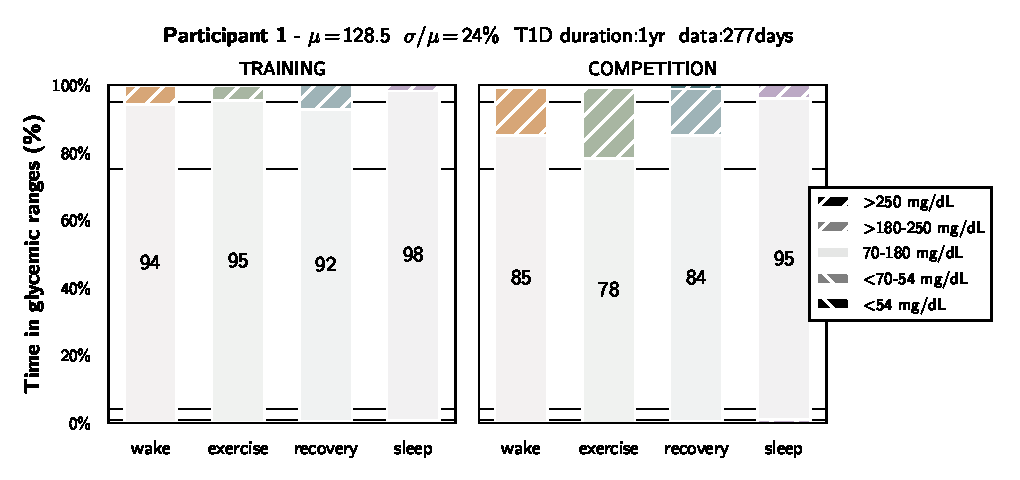
\includegraphics[width=.75\textwidth]{figure/time_in_zone/time_in_glucoselevel_traincomp_1.pdf}
    \end{subfigure}\vfill
    \begin{subfigure}{\textwidth}
        \centering
        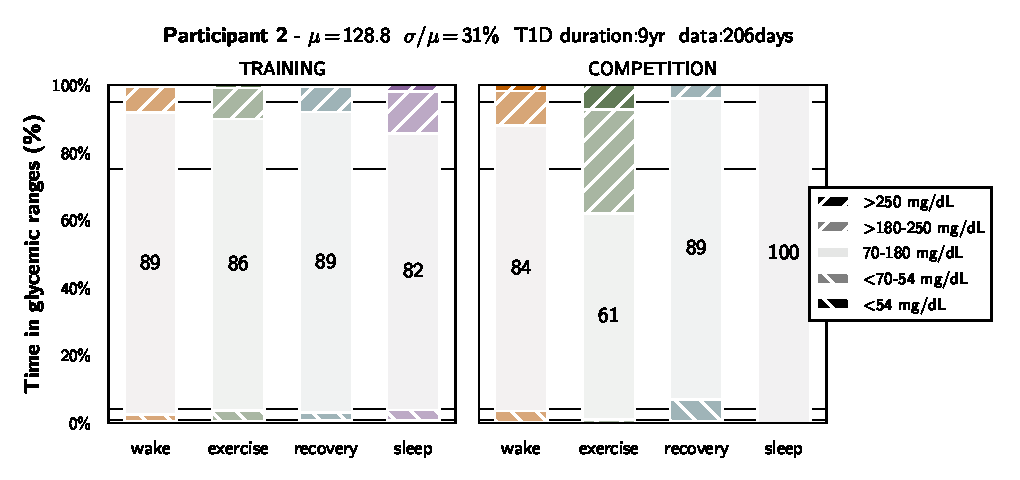
\includegraphics[width=.75\textwidth]{figure/time_in_zone/time_in_glucoselevel_traincomp_2.pdf}
    \end{subfigure}\vfill
    \begin{subfigure}{\textwidth}
        \centering
        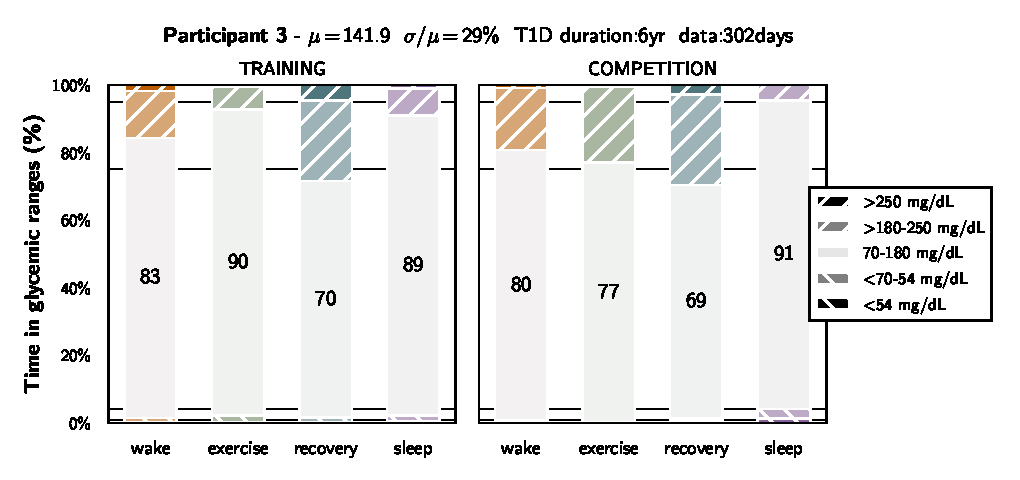
\includegraphics[width=.75\textwidth]{figure/time_in_zone/time_in_glucoselevel_traincomp_3.pdf}
    \end{subfigure}\vfill
    \begin{subfigure}{\textwidth}
        \centering
        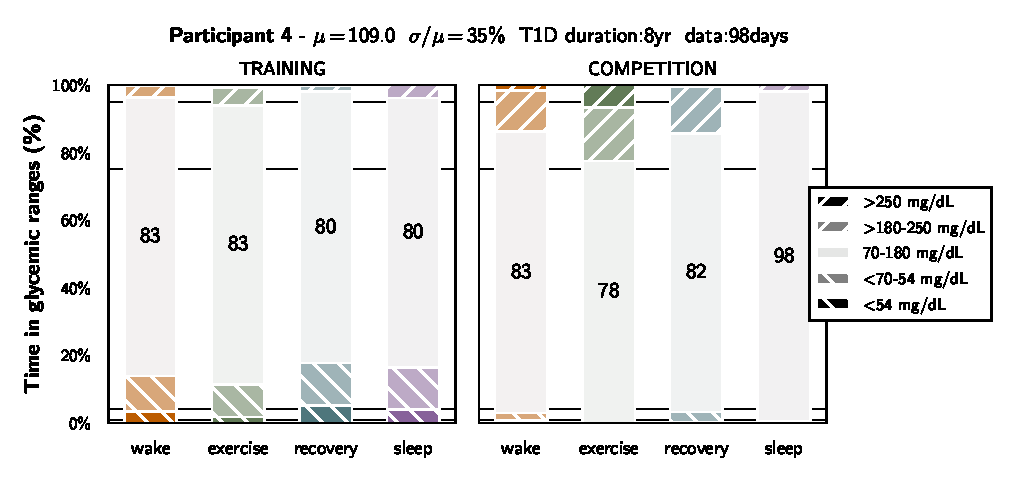
\includegraphics[width=.75\textwidth]{figure/time_in_zone/time_in_glucoselevel_traincomp_4.pdf}
    \end{subfigure}\vfill
\end{figure}
\begin{figure}\ContinuedFloat
    \centering
    \begin{subfigure}{\textwidth}
        \centering
        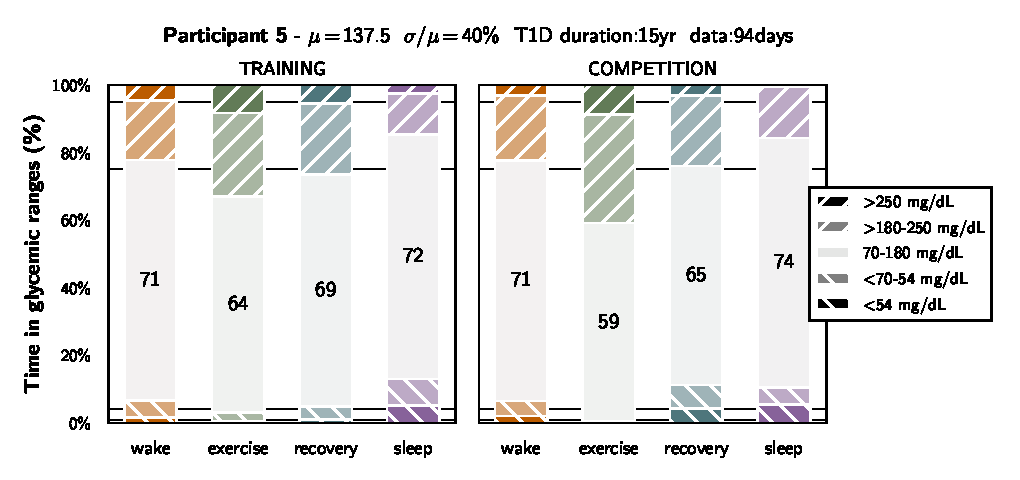
\includegraphics[width=.75\textwidth]{figure/time_in_zone/time_in_glucoselevel_traincomp_5.pdf}
    \end{subfigure}\vfill
    \begin{subfigure}{\textwidth}
        \centering
        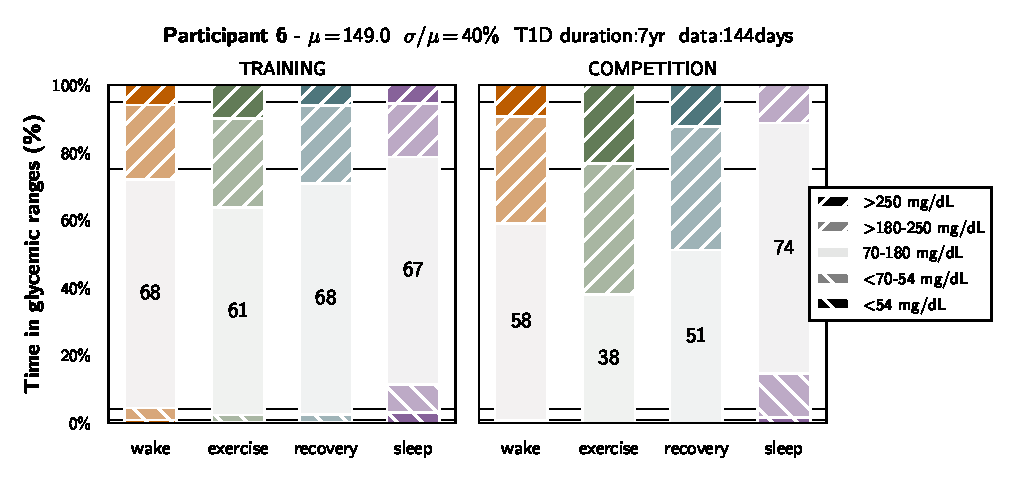
\includegraphics[width=.75\textwidth]{figure/time_in_zone/time_in_glucoselevel_traincomp_6.pdf}
    \end{subfigure}\vfill
    \begin{subfigure}{\textwidth}
        \centering
        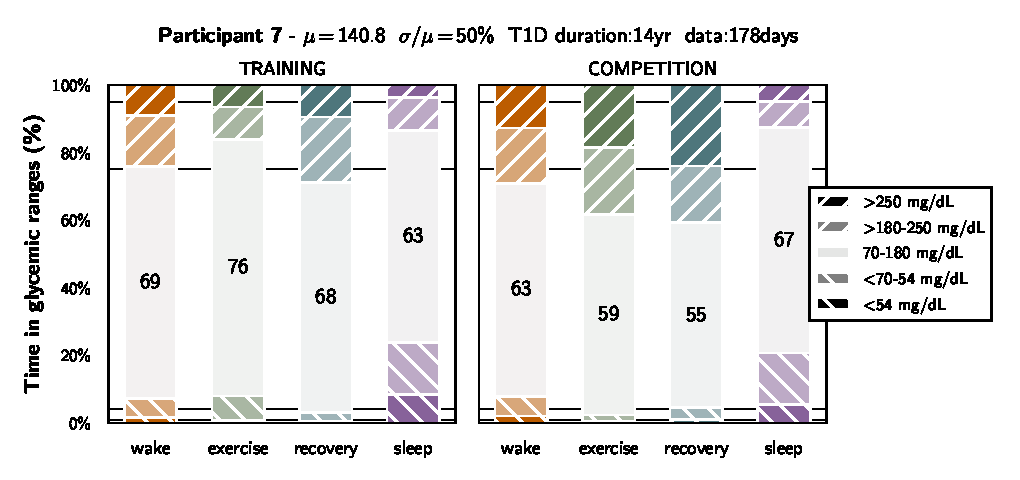
\includegraphics[width=.75\textwidth]{figure/time_in_zone/time_in_glucoselevel_traincomp_7.pdf}
    \end{subfigure}\vfill
    \begin{subfigure}{\textwidth}
        \centering
        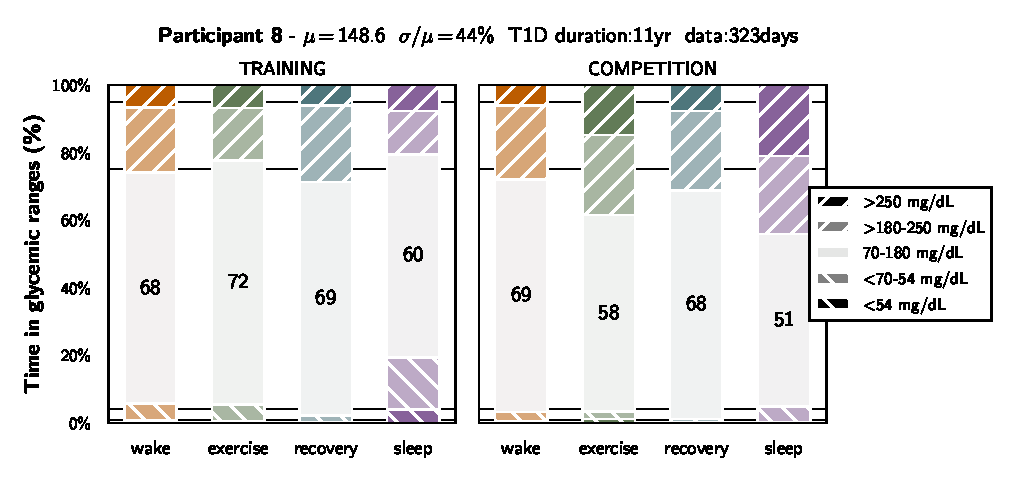
\includegraphics[width=.75\textwidth]{figure/time_in_zone/time_in_glucoselevel_traincomp_8.pdf}
    \end{subfigure}\vfill
\end{figure}
\begin{figure}\ContinuedFloat
    \centering
    \begin{subfigure}{\textwidth}
        \centering
        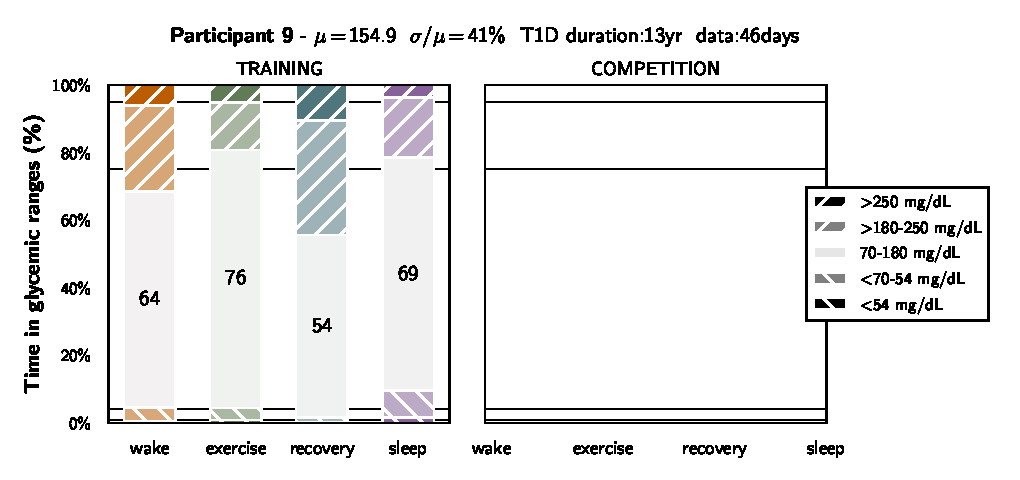
\includegraphics[width=.75\textwidth]{figure/time_in_zone/time_in_glucoselevel_traincomp_9.pdf}
    \end{subfigure}\vfill
    \begin{subfigure}{\textwidth}
        \centering
        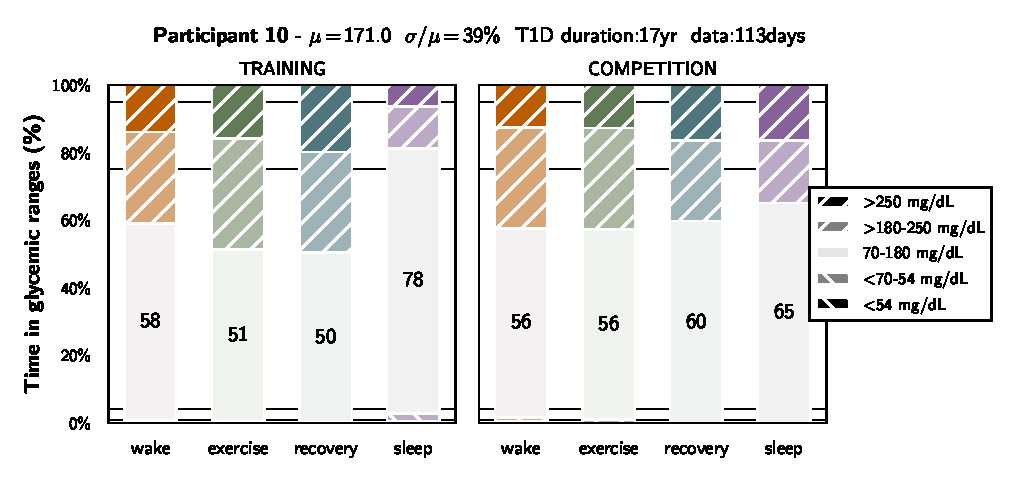
\includegraphics[width=.75\textwidth]{figure/time_in_zone/time_in_glucoselevel_traincomp_10.pdf}
    \end{subfigure}\vfill
    \begin{subfigure}{\textwidth}
        \centering
        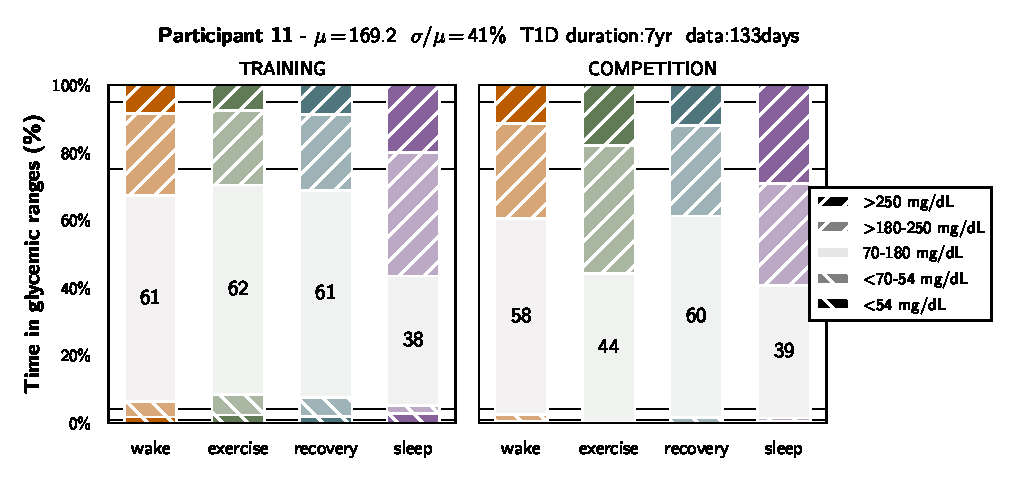
\includegraphics[width=.75\textwidth]{figure/time_in_zone/time_in_glucoselevel_traincomp_11.pdf}
    \end{subfigure}\vfill
    \begin{subfigure}{\textwidth}
        \centering
        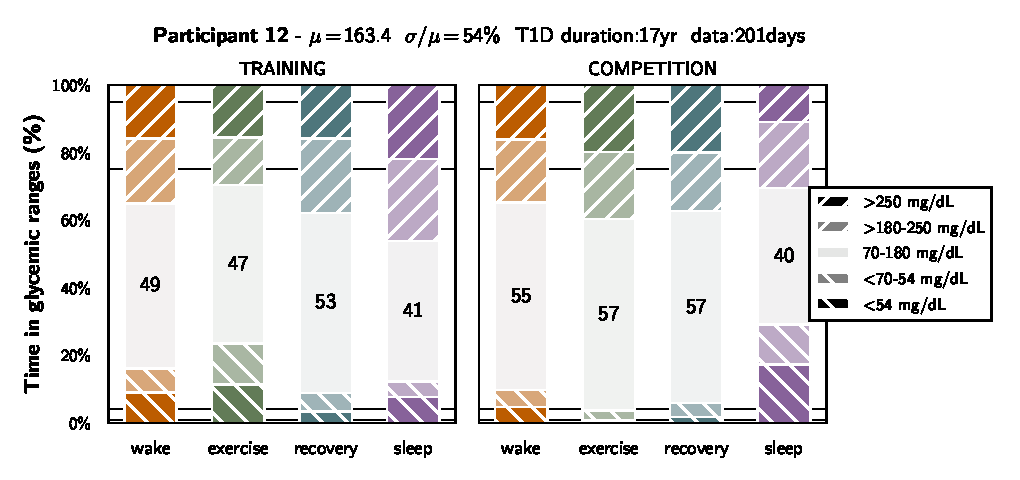
\includegraphics[width=.75\textwidth]{figure/time_in_zone/time_in_glucoselevel_traincomp_12.pdf}
    \end{subfigure}\vfill
\end{figure}

\begin{threeparttable}
    \caption{Number of participants that meet the clinical targets from \citet{31177185}.}
    \label{tab:targets-number}
    \scriptsize
    \centering
    \begin{tabular}{@{}l rc rc rc rc rc@{}}
        \toprule
        & \multicolumn{2}{c}{\textbf{Entire day}} & \multicolumn{2}{c}{\textbf{Wake}} & \multicolumn{2}{c}{\textbf{Exercise}} & \multicolumn{2}{c}{\textbf{Recovery}} & \multicolumn{2}{c}{\textbf{Sleep}}\\
        & \multicolumn{2}{c}{(06:00--06:00h)} & \multicolumn{2}{c}{(06:00--00:00h)} & & & \multicolumn{2}{c}{(4h post-exercise)} & \multicolumn{2}{c}{(00:00--06:00h)}\\
        \midrule
        \textbf{All days (2,115 obs.)}\\
        Mean glucose [mg/dL] & - & - & - & - & - & - & - & - & - & -\\
        Glycemic variability [\%]                         & 4 & [33.3\%] & 4 & [33.3\%] & 5 & [41.7\%] & 7 & [58.3\%] & 3 & [25.0\%]\\
        \textit{CGM readings [\%] in ...} \\
        ... hypoglycemia (<70 mg/dL)                      & 4 & [33.3\%] & 6 & [50.0\%] & 6 & [50.0\%] & 8 & [66.7\%] & 4 & [33.3\%] \\
        \hspace{3mm} ... hypoglycemia L2 (<54 mg/dL)      & 5 & [41.7\%] & 7 & [58.3\%] & 9 & [75.0\%] & 8 & [66.7\%] & 4 & [33.3\%] \\
        \hspace{3mm} ... hypoglycemia L1 (54-69 mg/dL)    & 4 & [33.3\%] & 4 & [33.3\%] & 5 & [41.7\%] & 8 & [66.7\%] & 4 & [33.3\%]\\
        ... target range (70-180 mg/dL)                   & 5 & [41.7\%] & 5 & [41.7\%] & 7 & [58.3\%] & 3 & [25.0\%] & 7 & [58.3\%]\\
        ... hyperglycemia (>180 mg/dL)                    & 6 & [50.0\%] & 5 & [41.7\%] & 7 & [58.3\%] & 3 & [25.0\%] & 9 & [75.0\%]\\
        \hspace{3mm} ... hyperglycemia L1 (181-250 mg/dL) & 7 & [58.3\%] & 7 & [58.3\%] & 8 & [66.7\%] & 4 & [33.3\%] & 10 & [83.3\%]\\
        \hspace{3mm} ... hyperglycemia L2 (>250 mg/dL)    & 5 & [41.7\%] & 5 & [41.7\%] & 4 & [33.3\%] & 5 & [41.7\%] & 7 & [58.3\%]\\
        \midrule
    
        \textbf{Training days (1,536 obs.)}\\
        Mean glucose [mg/dL] & - & - & - & - & - & - & - & - & - & -\\
        Glycemic variability [\%]                         & 4 & [33.3\%] & 4 & [33.3\%] & 5 & [41.7\%] & 7 & [58.3\%] & 4 & [33.3\%]\\
        \textit{CGM readings [\%] in ...} \\
        ... hypoglycemia (<70 mg/dL)                      & 4 & [33.3\%] & 4 & [33.3\%] & 6 & [50.0\%] & 8 & [66.7\%] & 4 & [33.3\%]\\
        \hspace{3mm} ... hypoglycemia L2 (<54 mg/dL)      & 5 & [41.7\%] & 7 & [58.3\%] & 9 & [75.0\%] & 8 & [66.7\%] & 4 & [33.3\%]\\
        \hspace{3mm} ... hypoglycemia L1 (54-69 mg/dL)    & 4 & [33.3\%] & 4 & [33.3\%] & 5 & [41.7\%] & 8 & [66.7\%] & 4 & [33.3\%]\\
        ... target range (70-180 mg/dL)                   & 5 & [41.7\%] & 5 & [41.7\%] & 7 & [58.3\%] & 4 & [33.3\%] & 6 & [50.0\%]\\
        ... hyperglycemia (>180 mg/dL)                    & 7 & [58.3\%] & 6 & [50.0\%] & 7 & [58.3\%] & 3 & [25.0\%] & 10 & 83.3[\%]\\
        \hspace{3mm} ... hyperglycemia L1 (181-250 mg/dL) & 7 & [58.3\%] & 8 & [66.7\%] & 8 & [66.7\%] & 4 & [33.3\%] & 10 & [83.3\%]\\
        \hspace{3mm} ... hyperglycemia L2 (>250 mg/dL)    & 5 & [41.7\%] & 5 & [41.7\%] & 4 & [33.3\%] & 4 & [33.3\%] & 7 & [58.3\%]\\    \midrule
    
        \textbf{Competition days (256 obs.)}\\
        Mean glucose [mg/dL] & - & - & - & - & - & - & - & - & - & -\\
        Glycemic variability [\%]                         & 4 & [36.4\%] & 5 & [45.5\%] & 8 & [72.7\%] & 6 & [54.5\%] & 6 & [54.5\%]\\
        \textit{CGM readings [\%] in ...} \\
        ... hypoglycemia (<70 mg/dL)                      & 7 & [63.6\%] & 8 & [72.7\%] & 11 & [100\%] & 7 & [63.6\%] & 5 & [45.5\%]\\
        \hspace{3mm} ... hypoglycemia L2 (<54 mg/dL)      & 8 & [72.7\%] & 8 & [72.7\%] & 10 & [90.9\%] & 8 & [72.7\%] & 6 & [54.5\%]\\
        \hspace{3mm} ... hypoglycemia L1 (54-69 mg/dL)    & 6 & [54.5\%] & 7 & [63.6\%] & 10 & [90.9\%] & 7 & [63.6\%] & 6 & [54.5\%]\\
        ... target range (70-180 mg/dL)                   & 5 & [45.5\%] & 5 & [45.5\%] & 3 & [27.3\%] & 3 & [27.3\%] & 6 & [54.5\%]\\
        ... hyperglycemia (>180 mg/dL)                    & 6 & [54.5\%] & 5 & [45.5\%] & 3 & [27.3\%] & 4 & [36.4\%] & 7 & [63.6\%]\\
        \hspace{3mm} ... hyperglycemia L1 (181-250 mg/dL) & 7 & [63.6\%] & 7 & [63.6\%] & 3 & [27.3\%] & 5 & [45.5\%] & 9 & [81.8\%]\\
        \hspace{3mm} ... hyperglycemia L2 (>250 mg/dL)    & 5 & [45.5\%] & 5 & [45.5\%] & 2 & [18.2\%] & 5 & [45.5\%] & 7 & [63.6\%]\\
        \bottomrule
    \end{tabular}
\begin{tablenotes}
\item \footnotesize {Number of participants that met the clinical targets from \citet{31177185} on glycemic control over a competitive season. We distinguished between all days (2,115 observations), training days (1,536 observations), and competition days (256 observations). Statistics were calculated for five phases of the day: entire day, wake, exercise, recovery, and sleep. Data are n [\%].}
\end{tablenotes}
\end{threeparttable}

\newpage
\hspace*{-1.2cm}
\begin{threeparttable}
    \caption[Statistical comparison of glycemic outcomes with clinical targets]{Results of one-sample \textit{t}-tests to compare glycemic outcomes with clinical targets from \citet{31177185}.}
    \label{tab:ttest-onesamp}
    \scriptsize
    \centering
    \begin{tabular}{@{}l rl rl rl rl rl@{}}
        \toprule
        & \multicolumn{2}{c}{\textbf{Entire day}} & \multicolumn{2}{c}{\textbf{Wake}} & \multicolumn{2}{c}{\textbf{Exercise}} & \multicolumn{2}{c}{\textbf{Recovery}} & \multicolumn{2}{c}{\textbf{Sleep}}\\
        & \multicolumn{2}{c}{(06:00--06:00h)} & \multicolumn{2}{c}{(06:00--00:00h)} & & & \multicolumn{2}{c}{(4h post-exercise)} & \multicolumn{2}{c}{(00:00--06:00h)}\\
        & \textit{t} & \textit{p}-value & \textit{t} & \textit{p}-value & \textit{t} & \textit{p}-value & \textit{t} & \textit{p}-value & \textit{t} & \textit{p}-value \\ 
        \midrule
        \textbf{All days (2,115 obs.)}\\
        Mean glucose [mg/dL] & \multicolumn{1}{c}{-} & \multicolumn{1}{c}{-} & \multicolumn{1}{c}{-} & \multicolumn{1}{c}{-} & \multicolumn{1}{c}{-} & \multicolumn{1}{c}{-} & \multicolumn{1}{c}{-} & \multicolumn{1}{c}{-} & \multicolumn{1}{c}{-} & \multicolumn{1}{c}{-}\\
        Glycemic variability [\%]                         &  1.20 &  0.256 &  0.84 &  0.421 &  1.29 & \nl0.225     &  0.25 &  0.811 &  1.55 &  0.150   \\
        \textit{CGM readings [\%] in ...} \\
        ... hypoglycemia (<70 mg/dL)                      &  1.79 &  0.101 &  1.10 &  0.293 &  0.82	& \nl0.430     &  0.28 &  0.788 &  2.72 &  0.020 * \\
        \hspace{3mm} ... hypoglycemia L2 (<54 mg/dL)      &  1.45 &  0.176 &  0.92 &  0.379 &  0.47 & \nl0.649     &  0.29 &  0.775 &  2.39 &  0.036 * \\
        \hspace{3mm} ... hypoglycemia L1 (54-69 mg/dL)    &  1.73 &  0.112 &  1.07 &  0.308 &  1.03 & \nl0.325     &  0.26 &  0.797 &  2.50 &  0.030 * \\
        ... target range (70-180 mg/dL)                   & -0.01 &  0.992 &  0.03 &  0.980 &  0.09 & \nl0.933     & -0.50 &  0.630 & -0.09 &  0.929   \\
        ... hyperglycemia (>180 mg/dL)                    & -0.39 &  0.703 & -0.14 &  0.891 & -0.17 & \nl0.870     &  0.61 &  0.557 & -0.93 &  0.375   \\
        \hspace{3mm} ... hyperglycemia L1 (181-250 mg/dL) & -1.45 &  0.176 & -1.01 &  0.336 & -1.15 & \nl0.276     & -0.09 &  0.928 & -2.39 &  0.036 * \\
        \hspace{3mm} ... hyperglycemia L2 (>250 mg/dL)    &  1.07 &  0.309 &  1.13 &  0.284 &  1.42 & \nl0.183     &  1.49 &  0.165 &  0.70 &  0.495   \\
        \midrule
        \textbf{Training days (1,536 obs.)}\\
        Mean glucose [mg/dL] &\multicolumn{1}{c}{-} & \multicolumn{1}{c}{-} & \multicolumn{1}{c}{-} & \multicolumn{1}{c}{-} & \multicolumn{1}{c}{-} & \multicolumn{1}{c}{-} & \multicolumn{1}{c}{-} & \multicolumn{1}{c}{-} & \multicolumn{1}{c}{-} & \multicolumn{1}{c}{-}\\
        Glycemic variability [\%]                         &  1.16 &  0.270 &  0.82 &  0.430 &  1.23 & \nl0.245     &  0.06 &  0.953 &  1.42 &  0.183   \\
        \textit{CGM readings [\%] in ...} \\
        ... hypoglycemia (<70 mg/dL)                      &  2.01 &  0.069 &  1.32 &  0.215 &  1.14 & \nl0.277     &  0.34 &  0.743 &  2.85 &  0.016 * \\
        \hspace{3mm} ... hypoglycemia L2 (<54 mg/dL)      &  1.54 &  0.152 &  0.98 &  0.346 &  0.66 & \nl0.524     &  0.30 &  0.768 &  2.70 &  0.021 * \\
        \hspace{3mm} ... hypoglycemia L1 (54-69 mg/dL)    &  1.99 &  0.072 &  1.37 &  0.197 &  1.44 & \nl0.177     &  0.35 &  0.735 &  2.56 &  0.027 * \\
        ... target range (70-180 mg/dL)                   &  0.24 &  0.813 &  0.35 &  0.734 &  0.44 & \nl0.667     & -0.33 &  0.746 & -0.04 &  0.966   \\
        ... hyperglycemia (>180 mg/dL)                    & -0.81 &  0.433 & -0.63 &  0.542 & -0.77 & \nl0.458     &  0.43 &  0.677 & -1.04 &  0.319   \\
        \hspace{3mm} ... hyperglycemia L1 (181-250 mg/dL) & -1.82 &  0.096 & -1.47 &  0.170 & -1.73 & \nl0.112     & -0.18 &  0.864 & -2.25 &  0.046 * \\
        \hspace{3mm} ... hyperglycemia L2 (>250 mg/dL)    &  0.74 &  0.474 &  0.75 &  0.466 &  0.97 & \nl0.355     &  1.29 &  0.223 &  0.57 &  0.577   \\
        \midrule
        \textbf{Competition days (256 obs.)}\\
        Mean glucose [mg/dL] &\multicolumn{1}{c}{-} & \multicolumn{1}{c}{-} & \multicolumn{1}{c}{-} & \multicolumn{1}{c}{-} & \multicolumn{1}{c}{-} & \multicolumn{1}{c}{-} & \multicolumn{1}{c}{-} & \multicolumn{1}{c}{-} & \multicolumn{1}{c}{-} & \multicolumn{1}{c}{-}\\
        Glycemic variability [\%]                         &  0.42 &  0.684 & -0.03 &  0.979 & -1.01 & \nl0.336     & -0.07 &  0.949 &  0.19 &  0.856   \\
        \textit{CGM readings [\%] in ...} \\
        ... hypoglycemia (<70 mg/dL)                      &  0.53 &  0.609 & -0.40 &  0.701 & -6.76 &   <0.001 *** & -0.64 &  0.538 &  1.33 &  0.212   \\
        \hspace{3mm} ... hypoglycemia L2 (<54 mg/dL)      &  0.76 &  0.466 &  0.18 &  0.861 & -6.16 &   <0.001 *** & -0.59 &  0.570 &  1.21 &  0.255   \\
        \hspace{3mm} ... hypoglycemia L1 (54-69 mg/dL)    &  0.25 &  0.810 & -0.78 &  0.454 & -6.68 &   <0.001 *** & -0.61 &  0.559 &  1.19 &  0.260   \\
        ... target range (70-180 mg/dL)                   &  0.02 &  0.986 & -0.18 &  0.860 & -2.44 & \nl0.035 *   & -0.72 &  0.488 &  0.33 &  0.750   \\
        ... hyperglycemia (>180 mg/dL)                    &  0.05 &  0.958 &  0.59 &  0.566 &  3.47 & \nl0.006 **  &  1.08 &  0.306 & -0.87 &  0.406   \\
        \hspace{3mm} ... hyperglycemia L1 (181-250 mg/dL) & -0.86 &  0.409 &  0.04 &  0.969 &  2.79 & \nl0.019 *   &  0.14 &  0.892 & -2.62 &  0.026 * \\
        \hspace{3mm} ... hyperglycemia L2 (>250 mg/dL)    &  1.14 &  0.281 &  1.13 &  0.283 &  2.99 & \nl0.013 *   &  1.62 &  0.136 &  0.81 &  0.436   \\
        \bottomrule
    \end{tabular}
    \begin{tablenotes}
    \item \footnotesize {Results of one-sample \textit{t}-tests to compare glycemic outcomes with clinical targets from \citet{31177185} with a sample size of n=12. We distinguished between all days, training days, and competition days. Statistics were calculated for five phases of the day: entire day, wake, exercise, recovery, and sleep. Reported are \textit{t}-statistic and \textit{p}-value.}
    \vspace{1cm}
    \end{tablenotes}
\end{threeparttable}


\hspace*{-1.2cm}
\begin{threeparttable}
    \caption[Statistical comparison of glycemic outcomes on training days with competition days]{Results of paired \textit{t}-tests to compare glycemic outcomes on training days with competition days.}
    \label{tab:ttest-rel}
    \scriptsize
    \centering
    \begin{tabular}{@{}l rl rl rl rl rl@{}}
        \toprule
        & \multicolumn{2}{c}{\textbf{Entire day}} & \multicolumn{2}{c}{\textbf{Wake}} & \multicolumn{2}{c}{\textbf{Exercise}} & \multicolumn{2}{c}{\textbf{Recovery}} & \multicolumn{2}{c}{\textbf{Sleep}}\\
        & \multicolumn{2}{c}{(06:00--06:00h)} & \multicolumn{2}{c}{(06:00--00:00h)} & & & \multicolumn{2}{c}{(4h post-exercise)} & \multicolumn{2}{c}{(00:00--06:00h)}\\
        & \textit{t} & \textit{p}-value & \textit{t} & \textit{p}-value & \textit{t} & \textit{p}-value & \textit{t} & \textit{p}-value & \textit{t} & \textit{p}-value \\ 
        \midrule
        Mean glucose [mg/dL]                              & -2.73 &  0.021 * & -3.51 &  0.006 ** & -6.55 &   <0.001 *** & -2.34 &  0.041 * & -0.44 &  0.672 \\
        Glycemic variability [\%]                         &  1.64 &  0.133   &  2.03 &  0.069    &  3.57 & \nl0.005 **  &  0.44 &  0.667   &  1.06 &  0.314 \\
        \textit{CGM readings [\%] in ...} \\
        ... hypoglycemia (<70 mg/dL)                      &  2.00 &  0.073   &  2.09 &  0.063    & 2.85  & \nl0.017 *   &  0.87 &  0.407   &  0.83 &  0.426 \\
        \hspace{3mm} ... hypoglycemia L2 (<54 mg/dL)      &  2.22 &  0.050   &  1.66 &  0.128    &  1.51 & \nl0.163     &  0.78 &  0.455   &  0.40 &  0.696 \\
        \hspace{3mm} ... hypoglycemia L1 (54-69 mg/dL)    &  1.87 &  0.091   &  2.02 &  0.071    &  3.64 & \nl0.005 **  &  0.87 &  0.403   &  1.01 &  0.335 \\
        ... target range (70-180 mg/dL)                   &  1.21 &  0.256   &  1.91 &  0.085    &  3.30 & \nl0.008 **  &  1.24 &  0.242   & -0.80 &  0.441 \\
        ... hyperglycemia (>180 mg/dL)                    & -3.08 &  0.012 * & -3.84 &  0.003 ** & -5.49 &   <0.001 *** & -1.66 &  0.127   &  0.04 &  0.966 \\
        \hspace{3mm} ... hyperglycemia L1 (181-250 mg/dL) & -3.05 &  0.012 * & -4.04 &  0.002 ** & -5.53 &   <0.001 *** & -1.09 &  0.300   &  0.66 &  0.521 \\
        \hspace{3mm} ... hyperglycemia L2 (>250 mg/dL)    & -1.44 &  0.182   & -1.47 &  0.173    & -3.26 & \nl0.009 **  & -1.40 &  0.193   & -0.51 &  0.619 \\
        \bottomrule
    \end{tabular}
    \begin{tablenotes}
    \item \footnotesize {Results of paired \textit{t}-tests to compare glycemic outcomes on training days with competition days for a sample size of n=11 (i.e., one participant did not engage in competitive exercise). Statistics were calculated for five phases of the day: entire day, wake, exercise, recovery, and sleep. Reported are \textit{t}-statistic and \textit{p}-value.}
    \end{tablenotes}
\end{threeparttable}


\begin{comment}
\newpage
\begin{threeparttable}
    \caption{\TODO{Results of one-sample Wilcoxon signed-rank test to compare glycemic outcomes with clinical targets from \citet{31177185}.}}
    \label{tab:targets-number}
    \scriptsize
    \centering
    \begin{tabular}{@{}l rl rl rl rl rl@{}}
        \toprule
        & \multicolumn{2}{c}{\textbf{Entire day}} & \multicolumn{2}{c}{\textbf{Wake}} & \multicolumn{2}{c}{\textbf{Exercise}} & \multicolumn{2}{c}{\textbf{Recovery}} & \multicolumn{2}{c}{\textbf{Sleep}}\\
        & \multicolumn{2}{c}{(06:00--06:00h)} & \multicolumn{2}{c}{(06:00--00:00h)} & & & \multicolumn{2}{c}{(4h post-exercise)} & \multicolumn{2}{c}{(00:00--06:00h)}\\
        & \textit{t} & \textit{p}-value & \textit{t} & \textit{p}-value & \textit{t} & \textit{p}-value & \textit{t} & \textit{p}-value & \textit{t} & \textit{p}-value \\ 
        \midrule
        \textbf{All days (2,115 obs.)}\\
        Mean glucose [mg/dL] & \\
        Glycemic variability [\%]            &  26.0 &  0.339 &  30.0 &  0.519 & 27.0 &  0.380    & 39.0 &  1.000 &  19.0 &  0.129   \\
        \textit{CGM readings [\%] in ...} \\
        ... hypoglycemia L2 (<54 mg/dL)      &  27.0 &  0.380 &  34.0 &  0.733 & 23.0 &  0.233    & 34.0 &  0.733 &  14.0 &  0.052   \\
        ... hypoglycemia L1 (54-69 mg/dL)    &  20.0 &  0.151 &  28.0 &  0.424 & 30.0 &  0.519    & 33.0 &  0.677 &  14.0 &  0.052   \\
        ... target range (70-180 mg/dL)      &  38.0 &  0.970 &  39.0 &  1.000 & 37.0 &  0.910    & 30.0 &  0.519 &  38.0 &  0.970   \\
        ... hyperglycemia L1 (181-250 mg/dL) &  24.0 &  0.266 &  30.0 &  0.519 & 27.0 &  0.380    & 34.0 &  0.733 &  12.0 &  0.034 * \\
        ... hyperglycemia L2 (>250 mg/dL)    &  31.0 &  0.569 &  26.0 &  0.339 & 22.0 &  0.204    & 23.0 &  0.233 &  38.0 &  0.970   \\
        \midrule
        \textbf{Training days (1,536 obs.)}\\
        Mean glucose [mg/dL] & \\
        Glycemic variability [\%]            &  26.0 &  0.339 &  30.0 &  0.519 & 25.0 &  0.301    & 37.0 &  0.910 &  22.0 &  0.204   \\
        \textit{CGM readings [\%] in ...} \\
        ... hypoglycemia L2 (<54 mg/dL)      &  24.0 &  0.266 &  37.0 &  0.910 & 29.0 &  0.470    & 32.0 &  0.622 &  11.0 &  0.027 * \\
        ... hypoglycemia L1 (54-69 mg/dL)    &  16.0 &  0.077 &  25.0 &  0.301 & 26.0 &  0.339    & 33.0 &  0.677 &  15.0 &  0.064   \\
        ... target range (70-180 mg/dL)      &  38.0 &  0.970 &  38.0 &  0.970 & 34.0 &  0.733    & 30.0 &  0.519 &  38.0 &  0.970   \\
        ... hyperglycemia L1 (181-250 mg/dL) &  20.0 &  0.151 &  24.0 &  0.266 & 19.0 &  0.129    & 32.0 &  0.622 &  14.0 &  0.052   \\
        ... hyperglycemia L2 (>250 mg/dL)    &  32.0 &  0.622 &  33.0 &  0.677 & 30.0 &  0.519    & 25.0 &  0.301 &  34.0 &  0.733   \\
        \midrule
        \textbf{Competition days (256 obs.)}\\
        Mean glucose [mg/dL] & \\
        Glycemic variability [\%]            &  30.0 &  0.831 &  31.0 &  0.898 & 23.0 &  0.413    & 31.0 &  0.898 &  33.0 &  1.000   \\
        ... hypoglycemia L2 (<54 mg/dL)      &  30.0 &  0.831 &  30.0 &  0.831 &  1.0 &  0.002 ** & 17.0 &  0.175 &  32.0 &  0.966   \\
        ... hypoglycemia L1 (54-69 mg/dL)    &  30.0 &  0.831 &  25.0 &  0.520 &  1.0 &  0.002 ** & 26.0 &  0.577 &  29.0 &  0.765   \\
        ... target range (70-180 mg/dL)      &  32.0 &  0.966 &  32.0 &  0.966 &  6.0 &  0.014 *  & 25.0 &  0.520 &  30.0 &  0.831   \\
        ... hyperglycemia L1 (181-250 mg/dL) &  25.0 &  0.520 &  33.0 &  1.000 &  9.0 &  0.032 *  & 28.0 &  0.700 &   9.0 &  0.032 * \\
        ... hyperglycemia L2 (>250 mg/dL)    &  20.0 &  0.278 &  21.0 &  0.320 &  9.0 &  0.032 *  & 18.0 &  0.206 &  28.0 &  0.700   \\
        \bottomrule
    \end{tabular}
\end{threeparttable}

\vspace{1cm}
\begin{threeparttable}
    \caption{\TODO{Results of paired Wilcoxon signed-rank test to compare competition with training days.}}
    \label{tab:targets-number}
    \scriptsize
    \centering
    \begin{tabular}{@{}l rl rl rl rl rl@{}}
        \toprule
        & \multicolumn{2}{c}{\textbf{Entire day}} & \multicolumn{2}{c}{\textbf{Wake}} & \multicolumn{2}{c}{\textbf{Exercise}} & \multicolumn{2}{c}{\textbf{Recovery}} & \multicolumn{2}{c}{\textbf{Sleep}}\\
        & \multicolumn{2}{c}{(06:00--06:00h)} & \multicolumn{2}{c}{(06:00--00:00h)} & & & \multicolumn{2}{c}{(4h post-exercise)} & \multicolumn{2}{c}{(00:00--06:00h)}\\
        & \textit{t} & \textit{p}-value & \textit{t} & \textit{p}-value & \textit{t} & \textit{p}-value & \textit{t} & \textit{p}-value & \textit{t} & \textit{p}-value \\ 
        \midrule
        Mean glucose [mg/dL]                 & -2.73 &  0.021 * & -3.51 &  0.006 ** & -6.55 &   <0.001 *** & -2.34 &  0.041 * & -0.44 &  0.672 \\
        Glycemic variability [\%]            &  1.64 &  0.133   &  2.03 &  0.069    &  3.57 & \nl0.005 **  &  0.44 &  0.667   &  1.06 &  0.314 \\
        \textit{CGM readings [\%] in ...} \\
        ... hypoglycemia L2 (<54 mg/dL)      &  2.22 &  0.050   &  1.66 &  0.128    &  1.51 & \nl0.163     &  0.78 &  0.455   &  0.40 &  0.696 \\
        ... hypoglycemia L1 (54-69 mg/dL)    &  1.87 &  0.091   &  2.02 &  0.071    &  3.64 & \nl0.005 **  &  0.87 &  0.403   &  1.01 &  0.335 \\
        ... target range (70-180 mg/dL)      &  1.21 &  0.256   &  1.91 &  0.085    &  3.30 & \nl0.008 **  &  1.24 &  0.242   & -0.80 &  0.441 \\
        ... hyperglycemia L1 (181-250 mg/dL) & -3.05 &  0.012 * & -4.04 &  0.002 ** & -5.53 &   <0.001 *** & -1.09 &  0.300   &  0.66 &  0.521 \\
        ... hyperglycemia L2 (>250 mg/dL)    & -1.44 &  0.182   & -1.47 &  0.173    & -3.26 & \nl0.009 **  & -1.40 &  0.193   & -0.51 &  0.619 \\
        \bottomrule
    \end{tabular}
\end{threeparttable}
\end{comment}
% TODO: align tables to center of page

\newpage
\subsection{Associations of exercise with dysglycemia} 
\subsubsection{Software} The analysis on the associations of exercise with dysglycemia was performed using the lme4 package version 1.1.27.1 \cite{lme4} in R version 3.4.4 \cite{R}. The code is publicly available on \TODO{GITHUBLINK}.

\subsubsection{Definition of exercise and environment variables}
Exercise and environment variables are described in Table~\ref{tab:reg-variables}. These variables were used as independent variables in the regression analysis for the associations of exercise with dysglycemia.
% refer to table 

\subsubsection{Definition of dysglycemia} We quantify dysglycemia into six binary variables: the occurrence of hypo- and hyperglycemia events during exercise, recovery and sleep. For the definitions of hypo- and hyperglycemia events, we follow \citet{29162583}: readings respectively below $70$ mg/dL or above $180$ mg/dL for at least 15 minutes (i.e., for Dexcom G6 \gls{cgm} corresponding to three consecutive readings above/below these thresholds). These variables were used as dependent variables in the regression analysis for the associations of exercise with dysglycemia.

\subsubsection{Regression equations}
The regression equation used in the analysis of the association between exercise and dysglycemia is
%\vspace{1cm}
\begin{equation}\label{eq:reg}
    \underbrace{\text{log }\frac{p_{id}}{1-p_{id}}}_{\text{odds of dysglycemia}} = \left(\beta_0 + \eqnmark[black]{node1}{{\alpha_0}_i}\right) + \underbrace{\left(\beta_1 + \eqnmark[black]{node2}{{\alpha_1}_i}\right){x_1}_{id}}_{\text{exercise variable of interest}} + \underbrace{\beta_2 {x_2}_{id} + \ldots + \beta_k {x_k}_{id}}_{\text{environmental variables}} + \epsilon_{id}
    \annotate[yshift=1em]{}{node1}{random intercept}
    \annotate[yshift=1em]{}{node2}{random slope}
\end{equation}
with $p_{id} = \mathds{P}(y_{id} = 1)$. In this model, we used a random intercept ${\alpha_0}_i$ and random slope ${\alpha_1}_i$ for the variable of interest to account for participant-specific variation. The exercise variable of interest ${x_1}_{id}$ is any of the variables under ``Competitive aspect'', ``Core exercise metrics'', ``Power'', and ``Heart rate'' in Table~\ref{tab:reg-variables}. For each exercise variable of interest, a separate model was fitted. Environmental variables ${x_2}_{id}, \ldots, {x_k}_{id}$ are all the variables under ``Environment'' in Table~\ref{tab:reg-variables}. All environmental variables were included in each model. 
The dependent variable in these models is binary, i.e., whether the event (hypo- or hyperglycemia) had occurred in the specified time window (exercise, recovery or sleep). For each individual exercise variable of interest, a total of six independent models were fitted, i.e., one for each of the two dysglycemia events during the three time windows.

\subsubsection{Results of association analysis}
The results of the above described regression analyses are summarized in two figures. The first figure shows only the estimated coefficients of all the exercise variables of interest $\hat{\beta_1}$ for all six events, referred to as the summary figure. The second figure shows all estimated coefficients $\hat{\beta_0},  \ldots, \hat{\beta_k}$ of all regressions, referred to as the full results. We emphasize that the first type of figure is a composite figure, comprising the results of multiple independent regression analyses. Hence, it should not be interpreted as the result of a single regression analysis.

Both figures show the estimated standardized associations of the exercise variables with the \gls{or} of hypo- and hyperglycemia during exercise, recovery and sleep. Listed are the odds ratio [95\% \gls{ci}] and \pval-value. Significance is indicated with *** (\pval<0.001), ** (\pval<0.01) and * (\pval<0.05). Associations are presented on a logarithmic scale and vary in color, where more color represents a stronger association. The colors blue and red demonstrate a decrease and increase in odds ratio, respectively.

For the association analysis presented in the manuscript, the summary figure can be found in the main manuscript Figure 2. The full results of this analysis are shown in Figure~\ref{fig:reg-main-full}. 

\subsubsection{Interpretation and limitations of association analysis}
We emphasize that the results of this analysis are associations, and not causal effects, due to the usage of observational data for this study. Moreover, we highlight that we fitted separate logistic regression models for each exercise variable individually. Through this design, we obtain associations of each exercise variable individually and prevent multi-collinearity due to high correlations among exercise variables. For this reason, we emphasize that the summary results of this analysis should not be interpreted as the results of a single regression analysis. 
%Finally, we note that we make the assumption that samples in this analysis are independent. However, due to the time series nature of our data, this assumption cannot be guaranteed.

\newpage
\renewcommand{\arraystretch}{1.25}
\begin{threeparttable}[hbtp]
    \caption{Description of exercise and environment variables.}
    \label{tab:reg-variables}
    \footnotesize
    \centering
    %\rowcolors{2}{white}{gray!25}
    \begin{tabular}{l p{3.5cm} c p{11.2cm}}
        \toprule
        %\rowcolor{gray!50}
        \multicolumn{2}{l}{\textbf{Variable}} & \textbf{Units} & \textbf{Description}\\
        \midrule
        \multicolumn{2}{l}{\textbf{Competitive aspect}}\\
        & Competition & [y/n] & Whether any exercise during the day was part of a competition.\\
        \multicolumn{2}{l}{\textbf{Core exercise metrics}}\\
        & Duration (T) & [s] & Total duration of all the exercises during the day.\\
        %& Normalised power (NP) & W & Power normalized for variability in cycling conditions to obtain a more accurate depiction of power expenditure, divided by the FTP, correcting for the fitness of an individual.\tnote{1} & $\text{NP} = \left( \frac{1}{T} \sum_{t\in T} \left( \frac{1}{30} \sum_{n=0}^{29} \text{P} (t-n) \right)^4\right)^{1/4}$\\%\cmidrule(lr){2-5}
        & Intensity factor (IF) & - & Power output normalized for variability in cycling conditions to obtain a more accurate depiction of power expenditure (i.e., \textit{normalized power}), which is divided by a participant's \gls{ftp} \cite{1937716155}, i.e., \begin{equation}\text{IF} = \left( \frac{1}{T} \sum_{t\in T} \left( \frac{1}{30} \sum_{n=0}^{29} \text{P} (t-n) \right)^4\right)^{1/4} \text{FTP}^{-1}\end{equation}\\
        %& Intensity factor (IF) & - & Normalized power corrected for the fitness of an individual.\tnote{1} & $\text{IF} = \text{NP}/ \text{FTP}$\\%\cmidrule(lr){2-5}
        %& Training stress score (TSS) & - & Estimate of load based on intensity and duration.\tnote{1} & $\text{TSS} = \left(\frac{T}{3600}\right) \cdot \text{IF}^2$\\%\cmidrule(lr){2-5}
        & Variability index (VI) & - & Metric for smoothness or variability of the power output during exercise, i.e., \begin{equation}\text{VI} = \left( \frac{1}{T} \sum_{t\in T} \left( \frac{1}{30} \sum_{n=0}^{29} \text{P} (t-n) \right)^4\right)^{1/4} \left[\frac{1}{T}\sum_{t\in T} P(t)\right]^{-1} \end{equation} \\
        %& Efficiency factor (EF) & W/bpm & & $\text{EF} = NP / \left[ \frac{1}{T}\sum_{t\in T} HR(t)\right]$\\%\cmidrule(lr){2-5}

        \multicolumn{2}{l}{\textbf{Power}}\\
        & Time in power zone ... & [min] & Time spent in personal Coggan power zones, based on fractions of the participant's \gls{ftp} \cite{1937716155}, i.e., \begin{equation}\sum_{t\in T} \boldsymbol{1}_{z}(P(t)) \text{ with } z = ...\end{equation}\\
        & ... 1 (Active recovery) & & ... $<56\%$ of \gls{ftp}\\ %$\sum_{t\in T} \boldsymbol{1}_{[0,\, 0.56\cdot FTP)}(P(t))$ \\%\cmidrule(lr){2-5}
        & ... 2 (Endurance) & & ... 56 to 76\% of \gls{ftp}\\%$\sum_{t\in T} \boldsymbol{1}_{[0.56\cdot FTP,\, 0.76\cdot FTP)}(P(t))$\\
        & ... 3 (Tempo) & & ... 76 to 91\% of \gls{ftp}\\ %$\sum_{t\in T} \boldsymbol{1}_{[0.76\cdot FTP,\, 0.91\cdot FTP)}(P(t))$ \\
        & ... 4 (Lactate threshold) & & ... 91 to 106\% of \gls{ftp}\\%$\sum_{t\in T} \boldsymbol{1}_{[0.91\cdot FTP,\, 1.06\cdot FTP)}(P(t))$ \\
        & ... 5 (VO\textsubscript{2max}) & & ... 106 to 121\% of \gls{ftp}\\%$\sum_{t\in T} \boldsymbol{1}_{[1.06\cdot FTP,\, 1.21\cdot FTP)}(P(t))$ \\
        & ... 6 (Anaerobic capacity) & & ... $>121\%$ of \gls{ftp}\\%$\sum_{t\in T} \boldsymbol{1}_{[1.21\cdot FTP,\, \infty )}(P(t))$ \\
        
        \multicolumn{2}{l}{\textbf{Heart rate}}\\
        & Time in heart rate zone ... & [min] & Time spent in personal Coggan heart rate zones, based on fractions of the participant's \gls{lthr} \cite{1937716155}, i.e.,  \begin{equation} \sum_{t\in T} \boldsymbol{1}_{z}(HR(t))  \text{ with } z = ... \end{equation}\\
        & ... 1 (Active recovery) & & ... $<69\%$ of \gls{lthr}\\%$\sum_{t\in T} \boldsymbol{1}_{[0,\, 0.69\cdot LTHR)}(HR(t))$ \\
        & ... 2 (Endurance) & & ... 69 to 84\% of \gls{lthr}\\%$\sum_{t\in T} \boldsymbol{1}_{[0.69\cdot LTHR,\, 0.84\cdot LTHR)}(HR(t))$ \\
        & ... 3 (Tempo) & & ... 84 to 95\% of \gls{lthr}\\%$\sum_{t\in T} \boldsymbol{1}_{[0.84\cdot LTHR,\, 0.95\cdot LTHR)}(HR(t))$ \\
        & ... 4 (Lactate threshold) & & ... 95 to 106\% of \gls{lthr}\\%$\sum_{t\in T} \boldsymbol{1}_{[0.95\cdot LTHR,\, 1.06\cdot LTHR)}(HR(t))$ \\
        & ... 5 (Anaerobic capacity) & & ... $>106\%$ of \gls{lthr}\\%$\sum_{t\in T} \boldsymbol{1}_{[1.06\cdot LTHR,\, \infty)}(HR(t))$\\
        \multicolumn{2}{l}{\textbf{Environment}}\\
        & Day in season & - & Day in the competitive season, starting from the participant's personal start of the season.\\
        & Travel & [y/n] & Whether any travelling has taken place on the respective day or the two days preceding it. Travel is defined as a change of countries, identified using the GPS location of the exercise, or a change of timezones, excluding any changes due to \gls{dst}.\\
        & Temperature & [\textdegree C] & Average temperature during the exercise.\\
        & Altitude & [m] & Average altitude of the exercise. \\
        \bottomrule
    \end{tabular}
    \begin{tablenotes}
    \footnotesize
    \item Quantities: $t$ = time [s]; $P(t)$ = power at time $t$ [W]; $HR(t)$ = heart rate at time $t$ [bpm]; FTP = functional threshold power [W]; LTHR = lactate threshold heart rate [bpm]; DST = daylight saving time.
    %\item For a more complete description of heart rate and power zones, see \citet{1937716155}.
    \end{tablenotes}
\end{threeparttable}


% ------------------------------ main
\newpage
\begin{figure}[hbtp!]
    \centering
    \caption[Full results of main association analysis]{Full results of main association analysis for the odds of \subrefb{fig:reg-main-hypo-full} hypoglycemia and \subrefb{fig:reg-main-hyper-full} hyperglycemia.}
    \label{fig:reg-main-full}
    \begin{subfigure}{\textwidth}
        \centering
        \caption{}
        \label{fig:reg-main-hypo-full}
        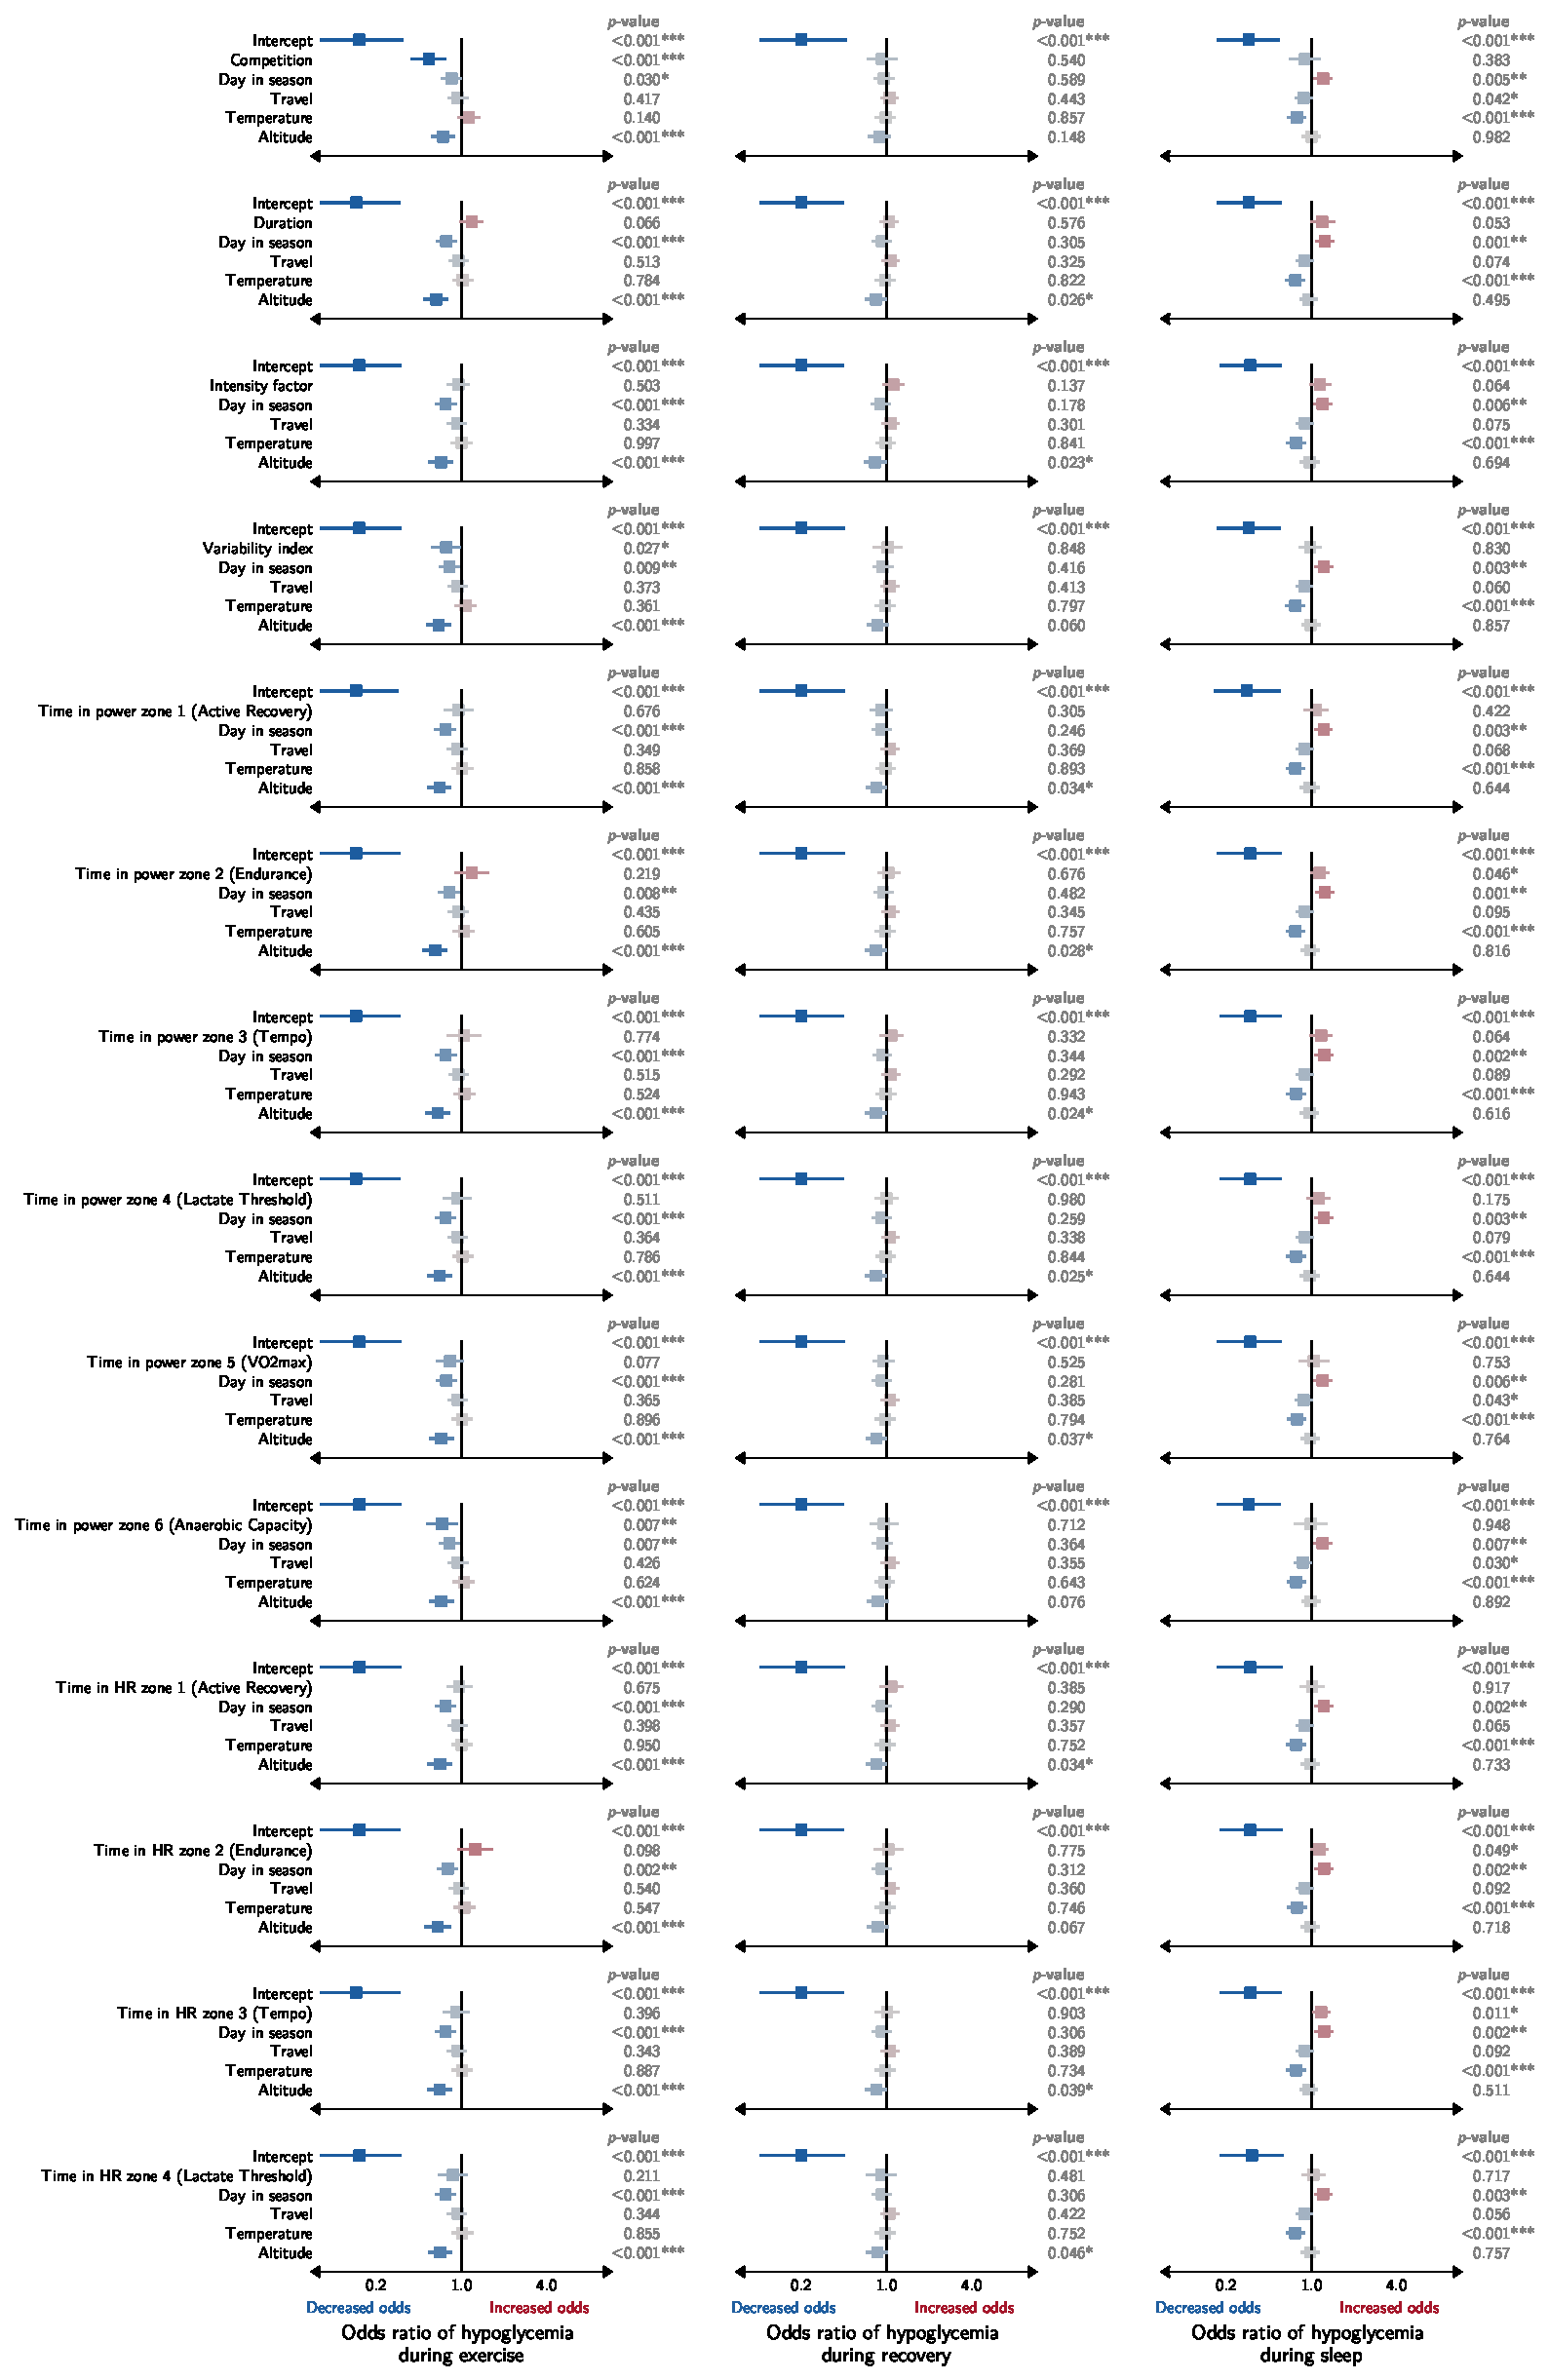
\includegraphics[width=\textwidth]{figure/main/coef_env_main_binomial_hypo.pdf}
    \end{subfigure}
\end{figure}
\begin{figure}[hbtp]\ContinuedFloat%[hbtp!]\ContinuedFloat
    \begin{subfigure}{\textwidth}
        \centering
        \caption{}
        \label{fig:reg-main-hyper-full}
        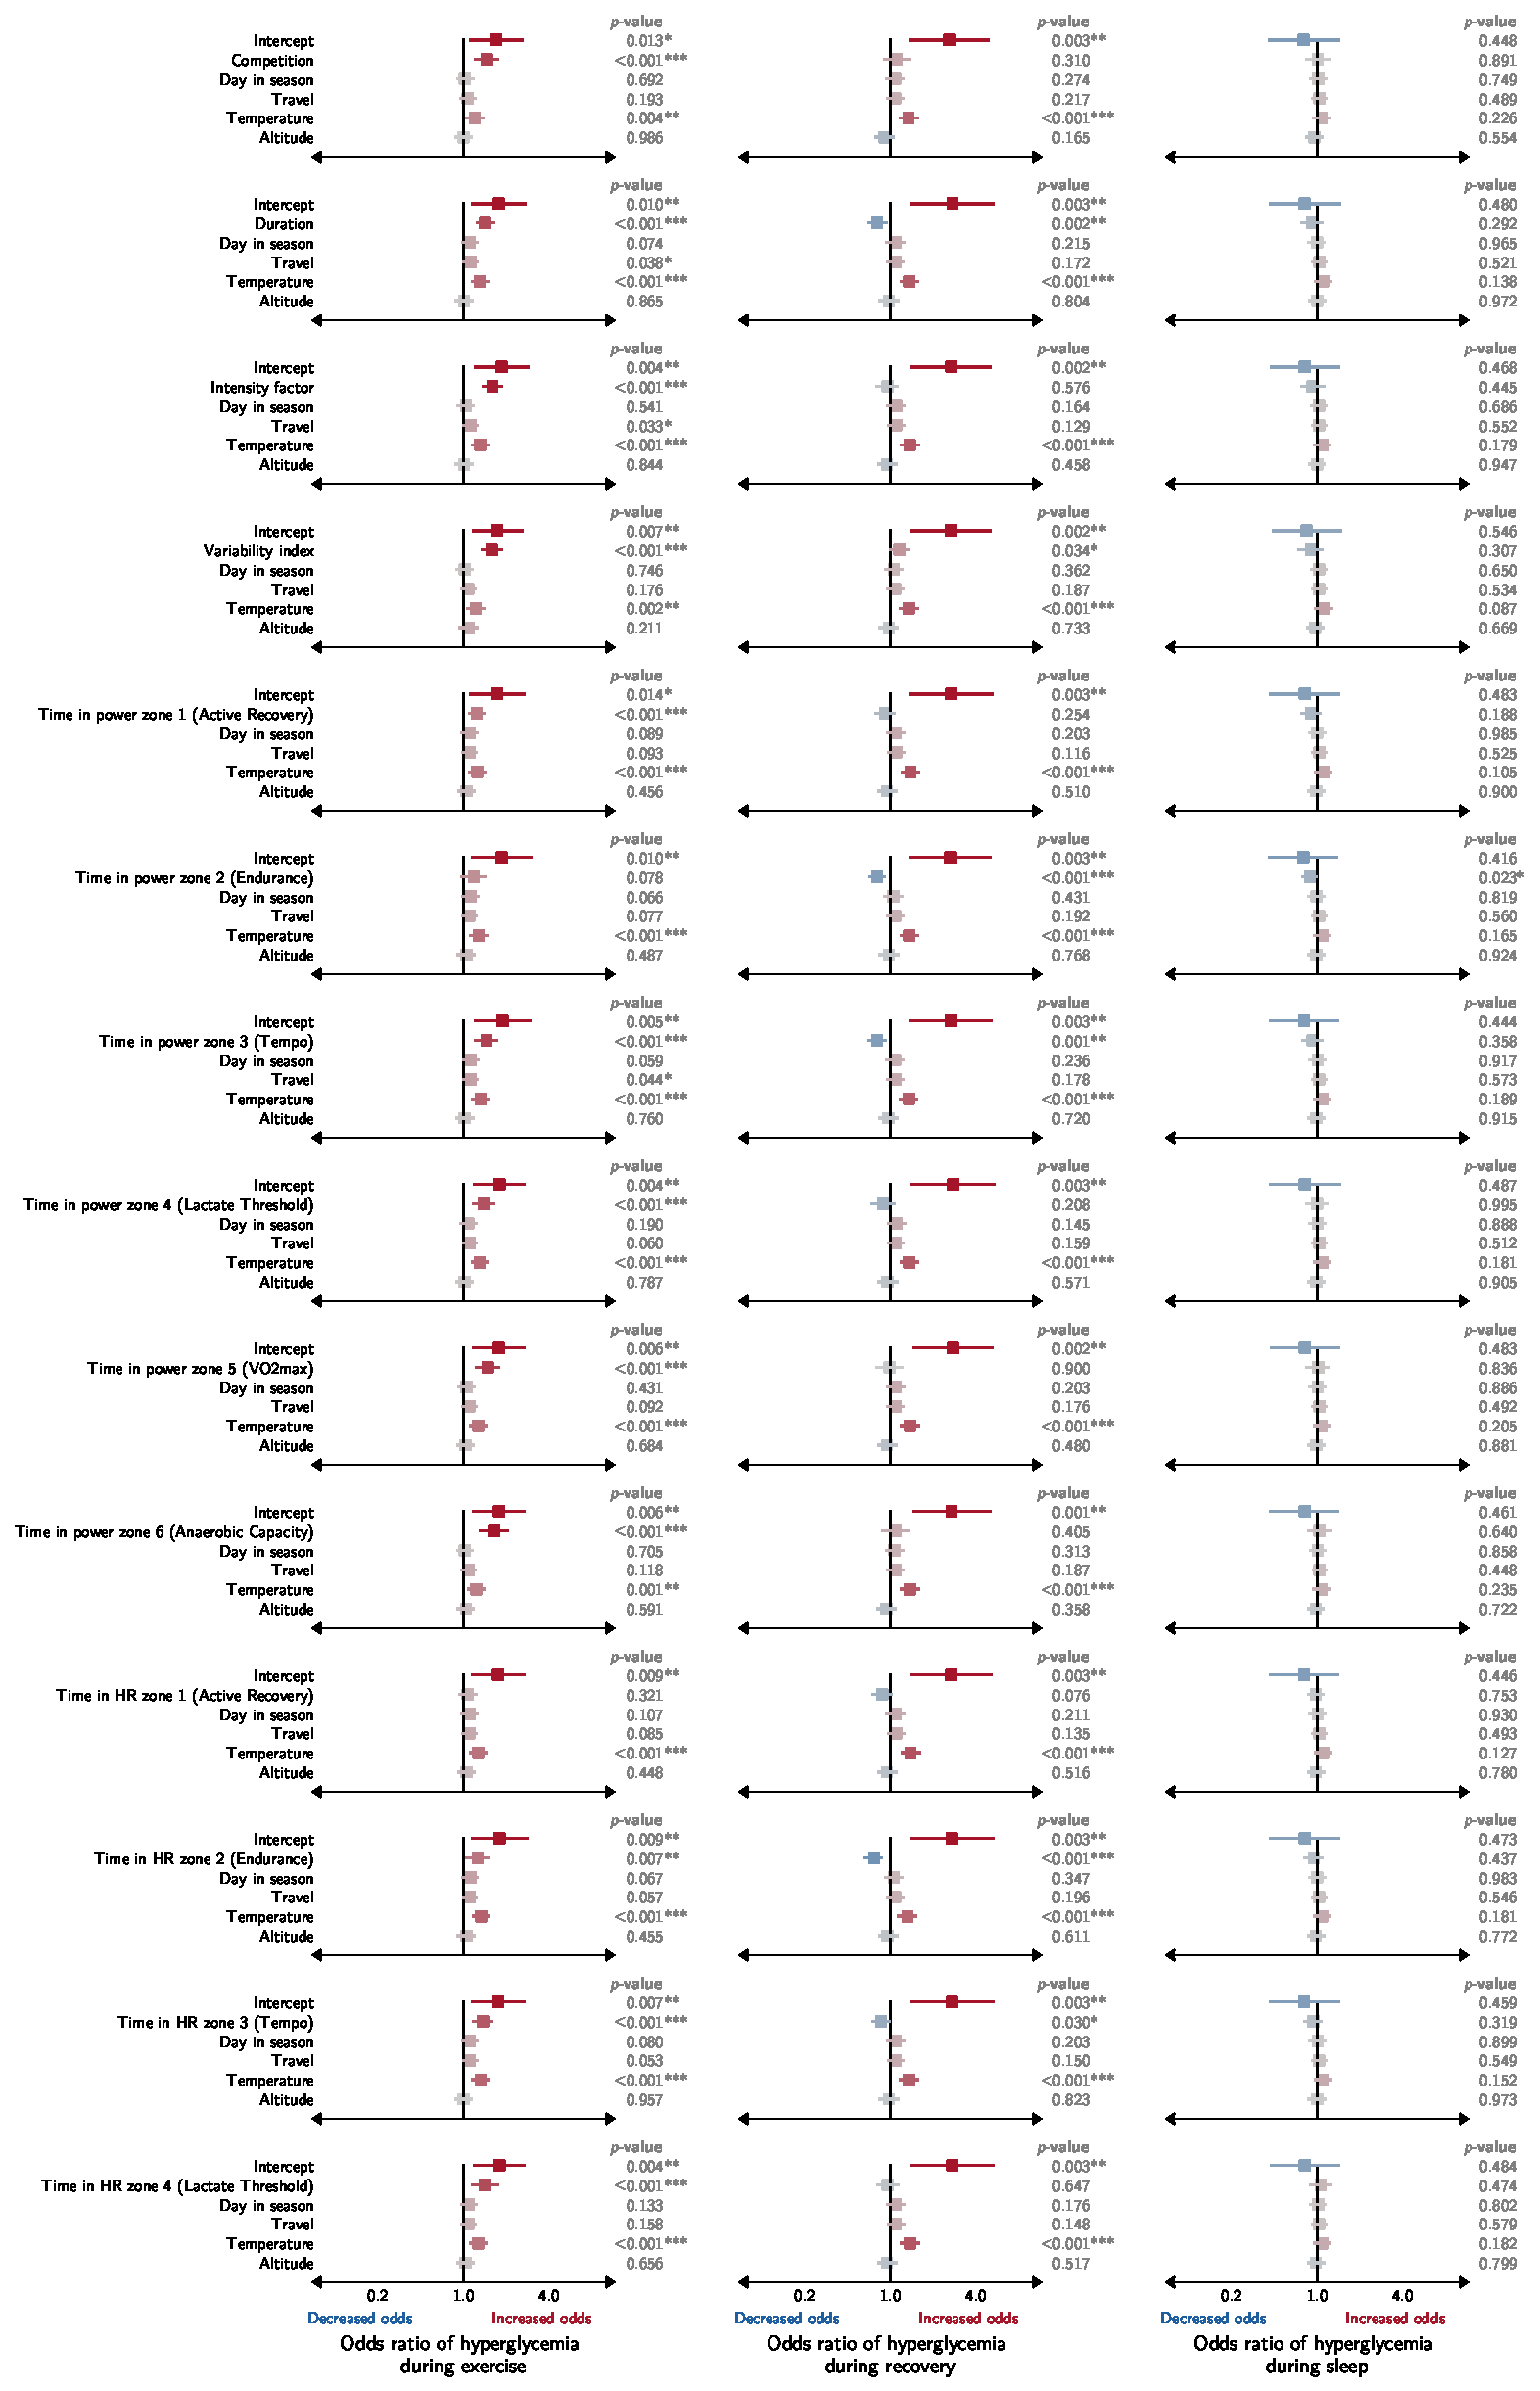
\includegraphics[width=\textwidth]{figure/main/coef_env_main_binomial_hyper.pdf}
    \end{subfigure}
\end{figure}

\newpage
\section{Supplementary analyses}
In addition to the analysis presented in the manuscript, we provide supplementary analyses to evaluate the validity and robustness of our results.

\subsection{Environmental variables}
%Here, we briefly comment on the associations of the environmental variables ${x_2}_{id}, \ldots, {x_k}_{id}$, as described in Table~\ref{tab:reg-variables}, with dysglycemia. 

\subsubsection{Associations of environmental variables with dysglycemia} In addition to the main analysis of the manuscript, we performed an analysis in which we investigated the associations of environmental variables ${x_2}_{id}, \ldots, {x_k}_{id}$, as described in Table~\ref{tab:reg-variables}, with dysglycemia exclusively. For this purpose, we excluded the exercise variable of interest ${x_1}_{id}$ from our regression equation (Eq.~\ref{eq:reg}), and used the following equation for this analysis:
\vspace{7mm}
\begin{equation}\label{eq:reg-env}
    \underbrace{\text{log }{\frac{p_{id}}{1-p_{id}}}}_{\text{odds of dysglycemia}} = \left(\beta_0 + \eqnmark[black]{node1}{{\alpha_0}_i}\right) + \underbrace{\beta_2 {x_2}_{id} + \ldots + \beta_k {x_k}_{id}}_{\text{environmental variables}} + \epsilon_{id}.
    \annotate[yshift=1em]{}{node1}{random intercept}
\end{equation}
Hence, as we did not iterate over possible exercise variables ${x_1}_{id}$, we performed six regression analyses in total: for the associations with hypo- and hyperglycemia, during exercise, recovery, and sleep. The associations are shown in Figure~\ref{fig:reg-env-full}. During exercise, associations with the odds of hypoglycemia are found for altitude (\gls{or} 0.71 [0.59--0.84]; \pval<0.001) and day in the season (\gls{or} 0.77 [0.67--0.89]; \pval<0.001). Additionally, associations with the odds of hyperglycemia during exercise are for temperature (\gls{or} 1.28 [1.13--1.44]; \pval<0.001). During recovery, we observe a weak association of altitude with the odds of hypoglycemia (\gls{or}; 0.85 [0.73--0.99] \pval=0.034) and a strong association of temperature with the odds of hyperglycemia (\gls{or} 1.37 [1.20--1.57]; \pval<0.001). Finally, during sleep, we found associations with the odds of hypoglycemia for day in the season (\gls{or} 1.22 [1.07--1.38]; \pval=0.003) and temperature (\gls{or} 0.77 [0.68--0.88]; \pval<0.001). 

\begin{figure}[H]
    \centering
    \caption[Full results of association analysis for environmental variables only]{Full results of association analysis for environmental variables only for the odds of \subrefb{fig:reg-env-hypo-full} hypoglycemia and \subrefb{fig:reg-env-hyper-full}  hyperglycemia.}
    \label{fig:reg-env-full}
    \begin{subfigure}{\textwidth}
        \centering
        \caption{}
        \label{fig:reg-env-hypo-full}
        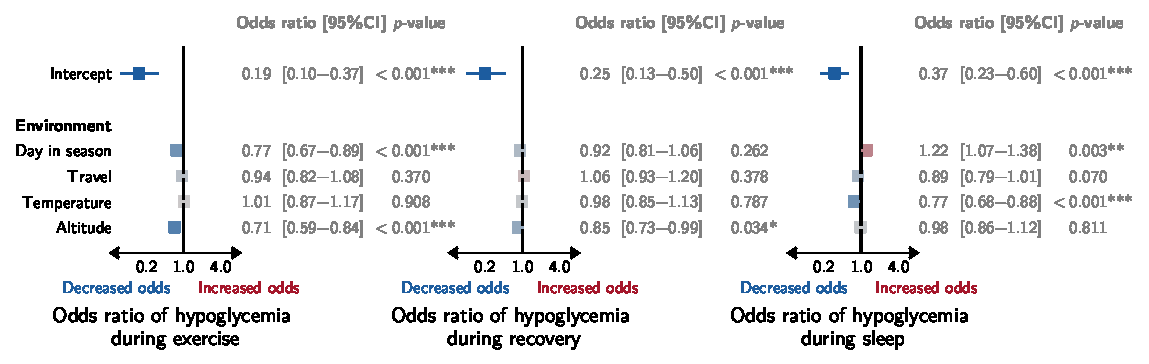
\includegraphics[width=.9\textwidth]{figure/env/coef_env_binomial_hypo.pdf}
    \end{subfigure}
    \begin{subfigure}{\textwidth}
        \centering
        \caption{}
        \label{fig:reg-env-hyper-full}
        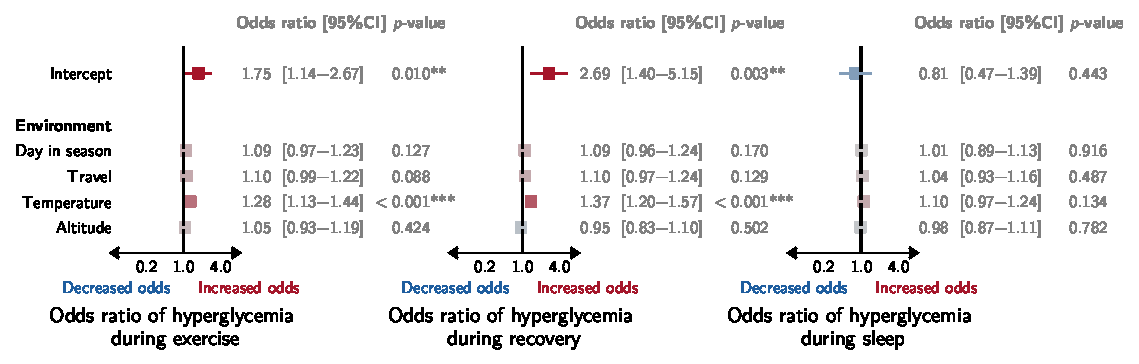
\includegraphics[width=.9\textwidth]{figure/env/coef_env_binomial_hyper.pdf}
    \end{subfigure}
\end{figure}

\newpage

\subsubsection{Exclusion of environmental variables}
To evaluate the robustness of our association models, we performed an additional analysis for the odds of dysglycemia where we excluded environmental variables. The regression model for this analysis is 
\vspace{7mm}
\begin{equation}\label{eq:reg-noenv}
    \underbrace{\text{log }{\frac{p_{id}}{1-p_{id}}}}_{\text{odds of dysglycemia}} = \left(\beta_0 + \eqnmark[black]{node1}{{\alpha_0}_i}\right) + \underbrace{\left(\beta_1 + \eqnmark[black]{node2}{{\alpha_1}_i}\right){x_1}_{id}}_{\text{exercise variable of interest}} + \epsilon_{id}.
    \annotate[yshift=1em]{}{node1}{random intercept}
    \annotate[yshift=1em]{}{node2}{random slope}
\end{equation}
The results of this analysis are shown in Figures~\ref{fig:reg-noenv} and \ref{fig:reg-noenv-full}.



% ------------------------------ noenv

\begin{figure}
    \centering
    \caption[Summary of association analysis with the exclusion of environmental variables]{Summary of association analysis with the exclusion of environmental variables for dysglycemia during \subrefb{fig:reg-noenv-exercise} exercise, \subrefb{fig:reg-noenv-recovery} recovery, and \subrefb{fig:reg-noenv-sleep} sleep.}
    \label{fig:reg-noenv}
    \begin{subfigure}{\textwidth}
        \centering
        \caption{}
        \label{fig:reg-noenv-exercise}
        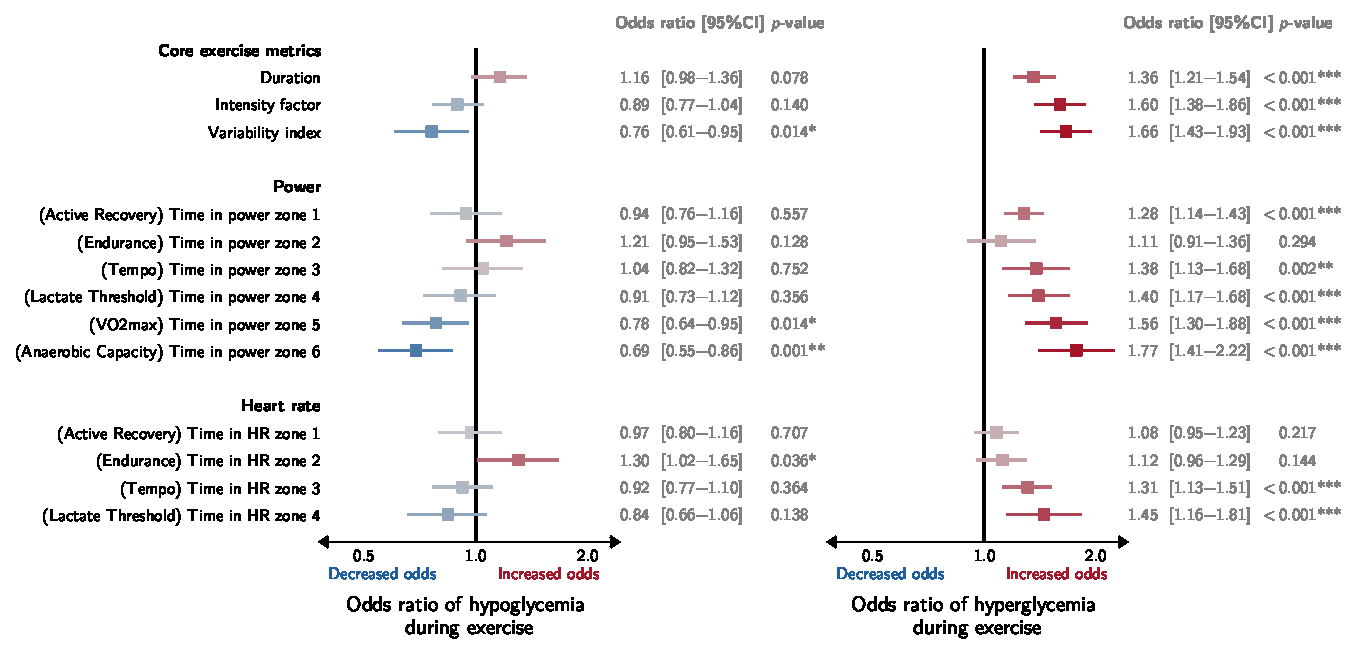
\includegraphics[trim=0cm 0cm 0cm 8mm, clip, width=.95\textwidth]{figure/noenv/coef_binomial_exercise.pdf}
    \end{subfigure}
    \begin{subfigure}{\textwidth}
        \centering
        \caption{}
        \label{fig:reg-noenv-recovery}
        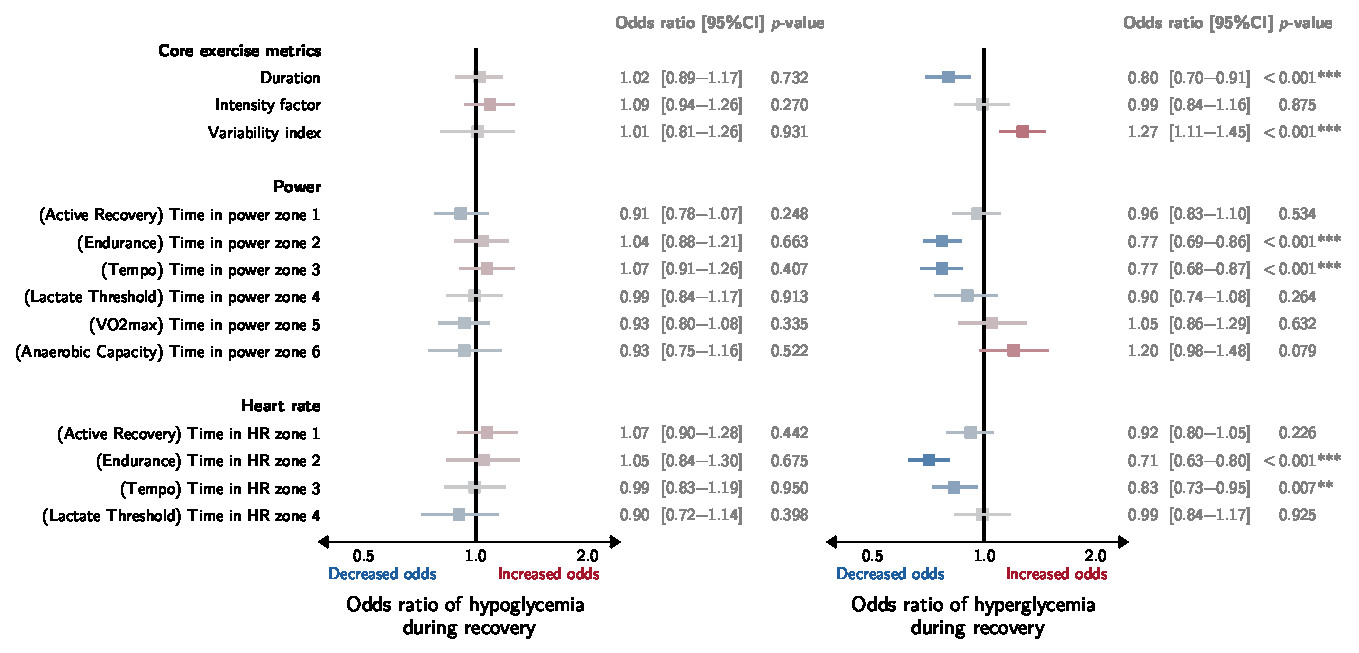
\includegraphics[trim=0cm 0cm 0cm 8mm, clip, width=.95\textwidth]{figure/noenv/coef_binomial_recovery.pdf}
    \end{subfigure}
    \begin{subfigure}{\textwidth}
        \centering
        \caption{}
        \label{fig:reg-noenv-sleep}
        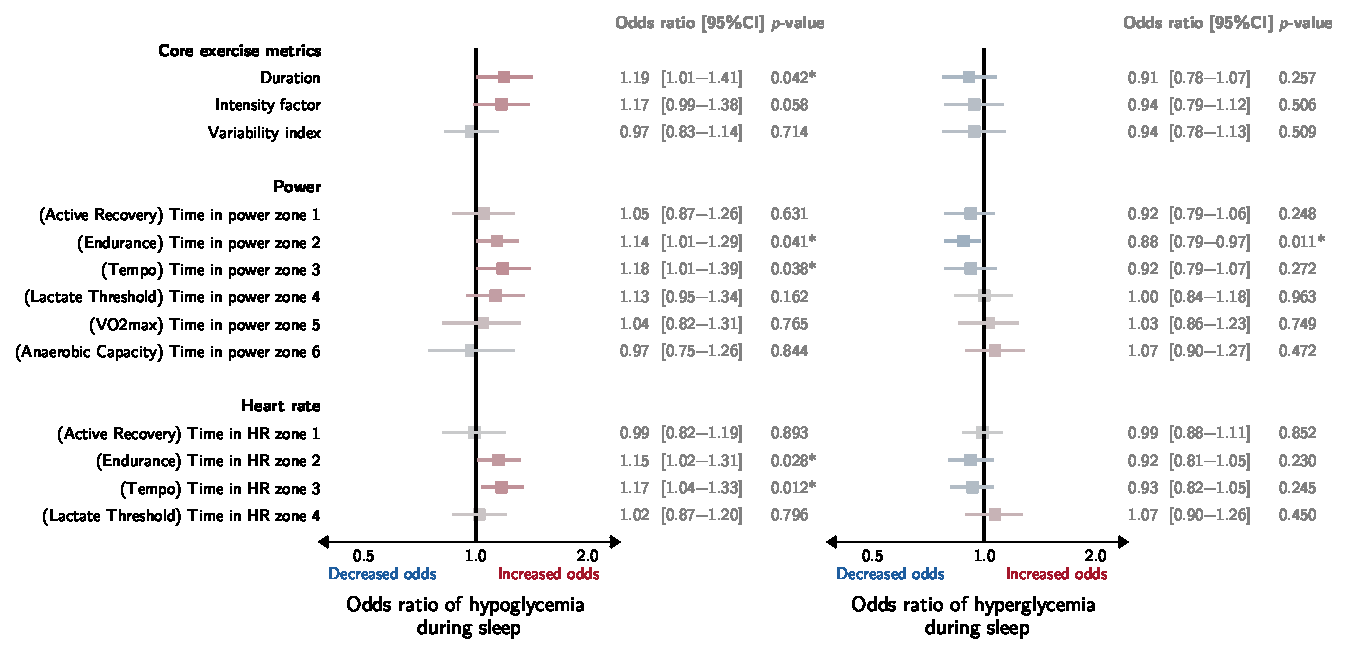
\includegraphics[trim=0cm 0cm 0cm 8mm, clip, width=.95\textwidth]{figure/noenv/coef_binomial_sleep.pdf}
    \end{subfigure}
\end{figure}

\begin{figure}[hbtp]
    \centering
    \caption[Full results of association analysis with the exclusion of environmental variables]{Full results of association analysis with the exclusion of environmental variables for the odds of \subrefb{fig:reg-noenv-hypo-full} hypoglycemia and \subrefb{fig:reg-noenv-hyper-full} hyperglycemia.}
    \label{fig:reg-noenv-full}
    \begin{subfigure}{\textwidth}
        \centering
        \caption{}
        \label{fig:reg-noenv-hypo-full}
        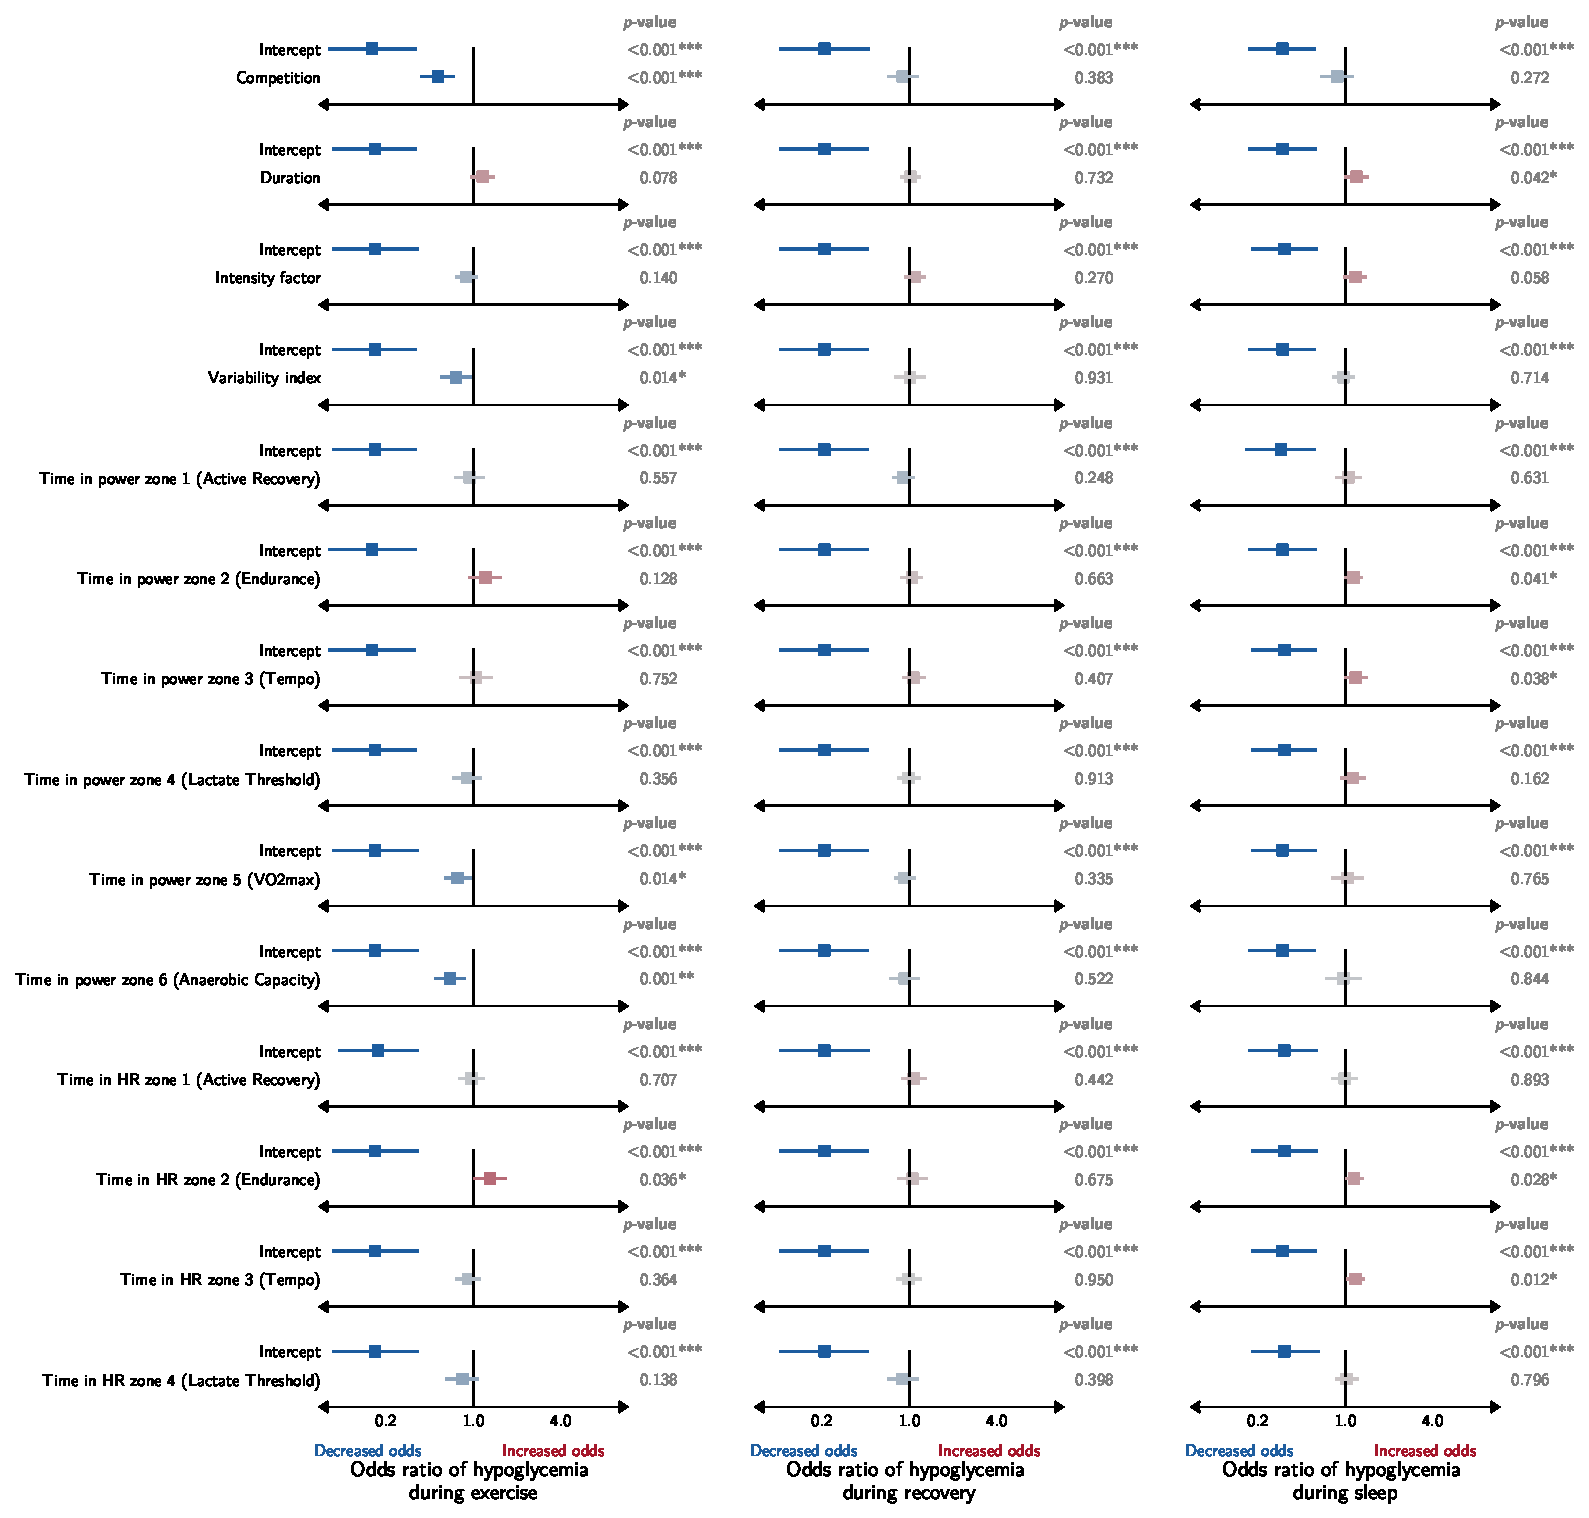
\includegraphics[width=\textwidth]{figure/noenv/coef_env_noenv_binomial_hypo.pdf}
    \end{subfigure}
\end{figure}
\begin{figure}[hbtp]\ContinuedFloat
    \begin{subfigure}{\textwidth}
        \centering
        \caption{}
        \label{fig:reg-noenv-hyper-full}
        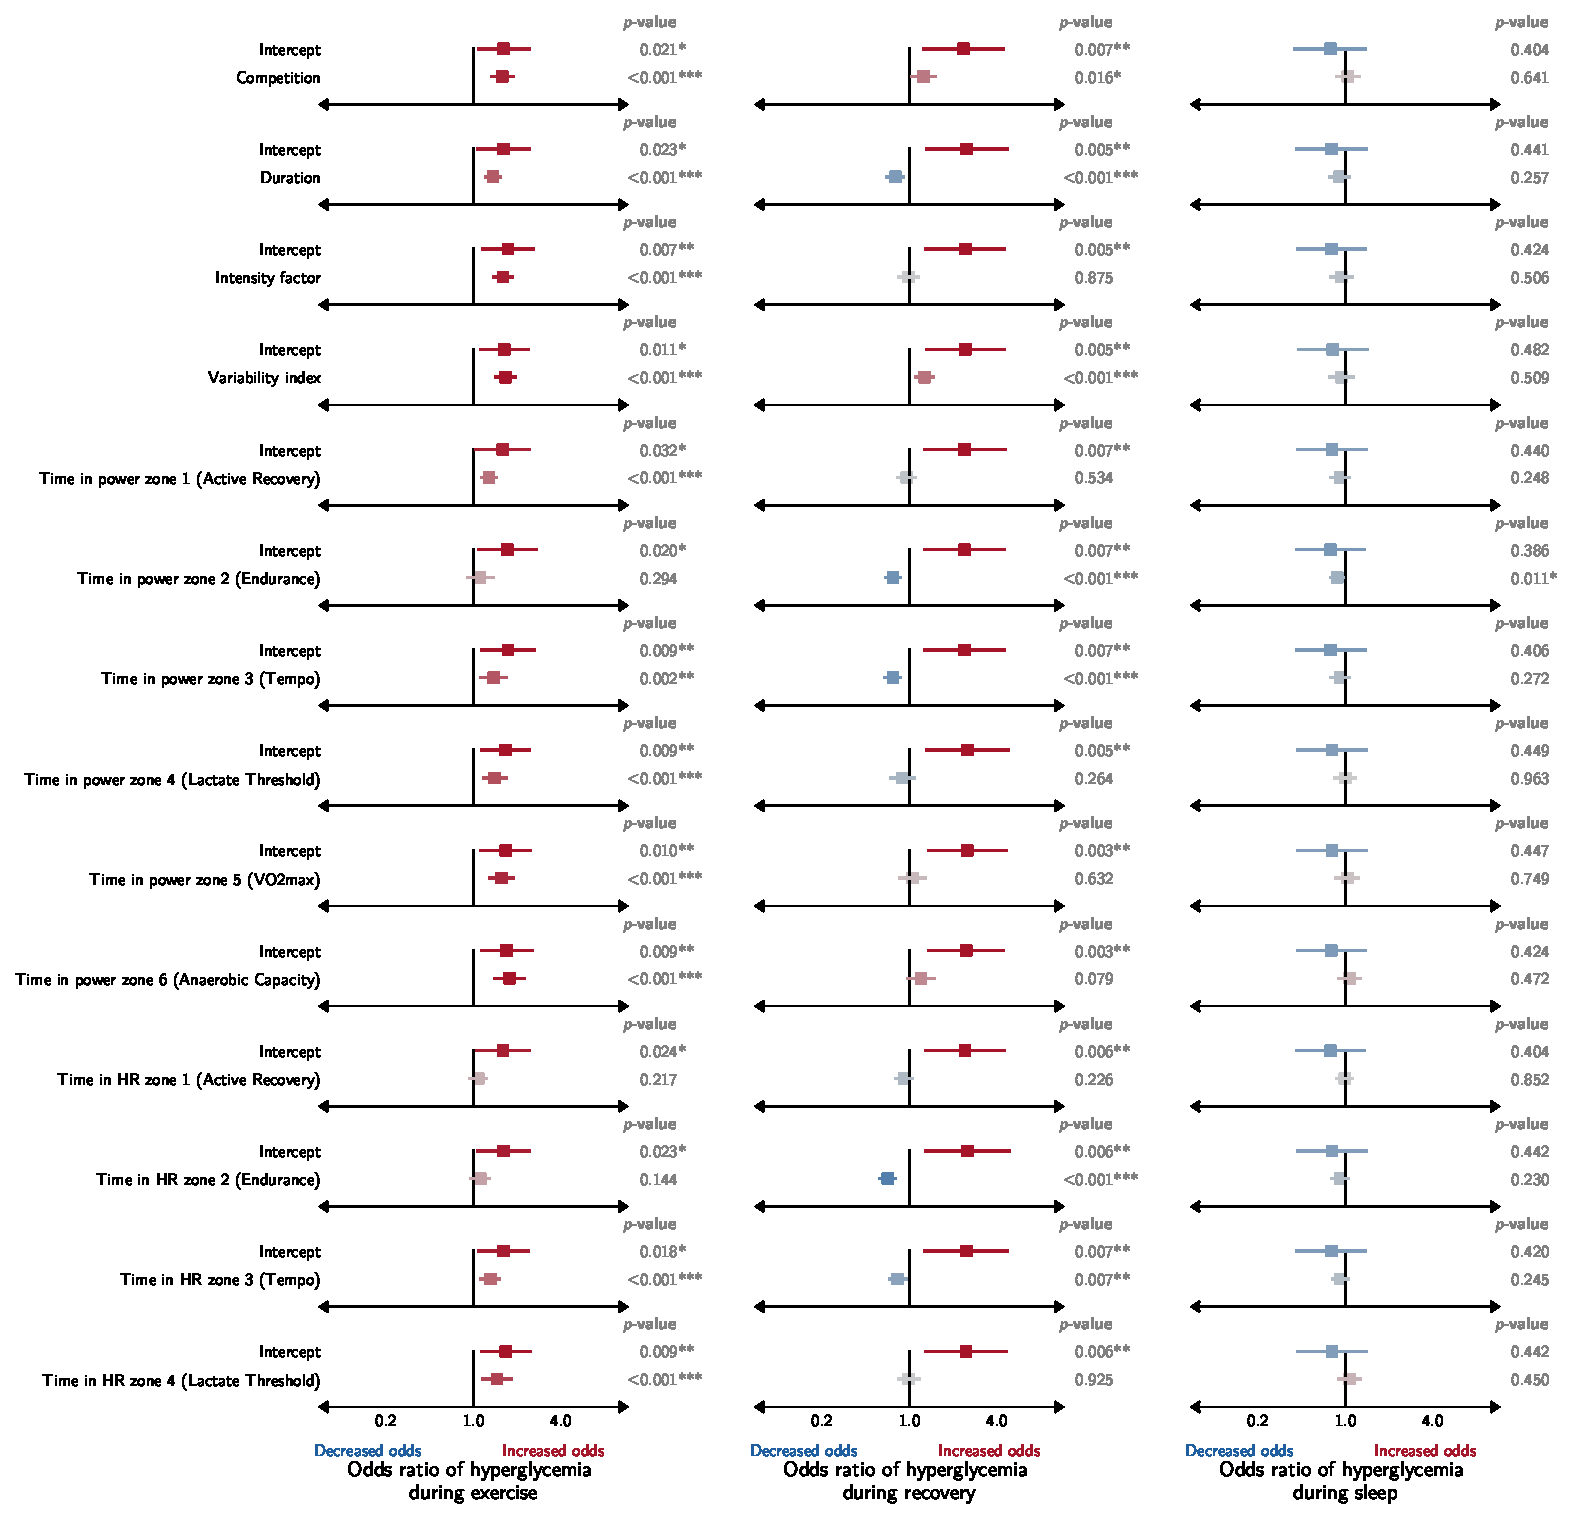
\includegraphics[width=\textwidth]{figure/noenv/coef_env_noenv_binomial_hyper.pdf}
    \end{subfigure}
\end{figure}

\subsection{Competitive aspect}
%Here, we comment on competitive aspect in the associations of exercise with dysglycemia. 

\subsubsection{Association of exercise variables with competition} 
In this analysis, we investigated the correlation between the variables in the categories ``Core exercise metrics'', ``Power'', and ``Heart rate'' with competition for individual exercise sessions. For this, we used a similar type of logistic regression as in Equation~\ref{eq:reg}, i.e.,
\vspace{1cm}
\begin{equation}\label{eq:reg-competition}
    \underbrace{\text{log }\frac{p_{id}}{1-p_{id}}}_{\text{odds of competition}} = \left(\beta_0 + \eqnmark[black]{node1}{{\alpha_0}_i}\right) + \underbrace{\left(\beta_1 + \eqnmark[black]{node2}{{\alpha_1}_i}\right){x_1}_{id}}_{\text{exercise variable of interest}} + \underbrace{\beta_2 {x_2}_{id} + \ldots + \beta_k {x_k}_{id}}_{\text{environmental variables}} + \epsilon_{id},
    \annotate[yshift=1em]{}{node1}{random intercept}
    \annotate[yshift=1em]{}{node2}{random slope}
\end{equation}
with $p_{id} = \mathds{P}(y_{id} = 1)$, where we included random intercepts ${\alpha_0}_i$ and random slopes ${\alpha_1}_i$ and control for environmental variables ${x_2}_{id}, \ldots, {x_k}_{id}$. Here, our dependent variable $y_{id}$ is competition (i.e., whether the exercise session was a competition), and our independent variable of interest ${x_1}_{id}$ is any of the exercise variables under ``Core exercise metrics'', ``Power'' and ``Heart rate'' in Table~\ref{tab:reg-variables}. Hence, multiple regression models were fitted, that is, one for each of the exercise variables. We report the results in a composite figure, where we report all estimated coefficients for the variable of interest $\hat{\beta_1}$. Figure~\ref{fig:reg-corr} shows these results. We find several significant strong associations of exercise variables and competition, where higher heart rate and power zones had stronger associations with the odds of competition.

\begin{figure}[H]
    \centering
    \caption{Summary of association analysis of exercise variables with competition.}
    \label{fig:reg-corr}
    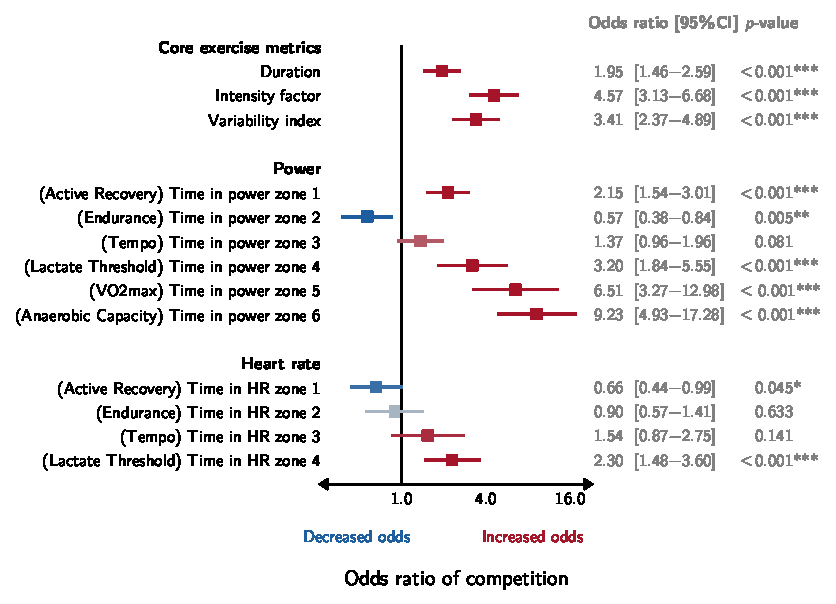
\includegraphics[width=.8\textwidth]{figure/corr/coef_corr_binomial_competition.pdf}
\end{figure}

\subsubsection{Stratification of competition and training days}
In the previous analysis, we found that there are strong associations with exercise variables and competition. Hence, we investigated potential differences in the associations (between exercise variables and dysglycemia) on competition days (256 observations) and on training days (1,536 observations). Thus, this analysis entails a stratification into training and competition days: the main association analysis is performed on training and competition days separately. The results of this analysis can be observed in Figures~\ref{fig:reg-train} and \ref{fig:reg-train-full} for training days and Figures~\ref{fig:reg-comp} and \ref{fig:reg-comp-full} for competition days. Similar patterns compared to the main analysis can be observed for training days. For competition days, only few variables were found to be significant, which may be due to the low number of competition days in this analysis. Strong significance for competition days was found between (i) duration and the odds of hyperglycemia during exercise (\gls{or} 0.59 [0.59--0.59]; \pval<0.001), (ii) duration and the odds of hypoglycemia during recovery (\gls{or} 0.81 [0.80--0.81]; \pval<0.001), and (iii) time in power zone 1 (active recovery) and the odds of hypoglycemia during sleep (\gls{or} 0.76 [0.76--0.77]; \pval<0.001).

%Despite strong associations between exercise variables and competition in the previous paragraph, the results of the association analysis in the main manuscript resemble the associations on training days the most. This is most likely driven by the large fraction of training days in the main analysis.  \TODO{Perhaps we should do an anova to compare the two models?}


% ------------------------------ train

\begin{figure}
    \centering
    \caption[Summary of association analysis on training days]{Summary of association analysis on training days for dysglycemia during \subrefb{fig:reg-train-exercise} exercise, \subrefb{fig:reg-train-recovery} recovery and \subrefb{fig:reg-train-sleep} sleep.}
    \label{fig:reg-train}
    \begin{subfigure}{\textwidth}
        \centering
        \caption{}
        \label{fig:reg-train-exercise}
        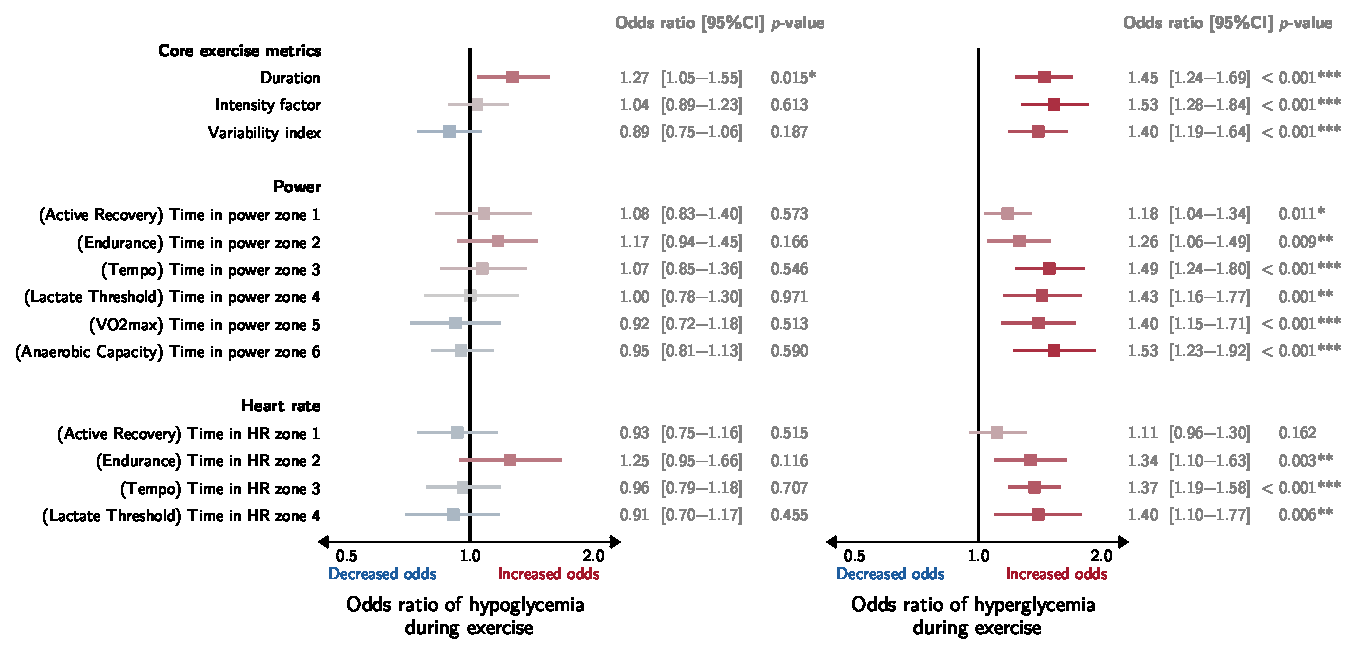
\includegraphics[trim=0cm 0cm 0cm 8mm, clip, width=.95\textwidth]{figure/train/coef_binomial_exercise.pdf}
    \end{subfigure}
    \begin{subfigure}{\textwidth}
        \centering
        \caption{}
        \label{fig:reg-train-recovery}
        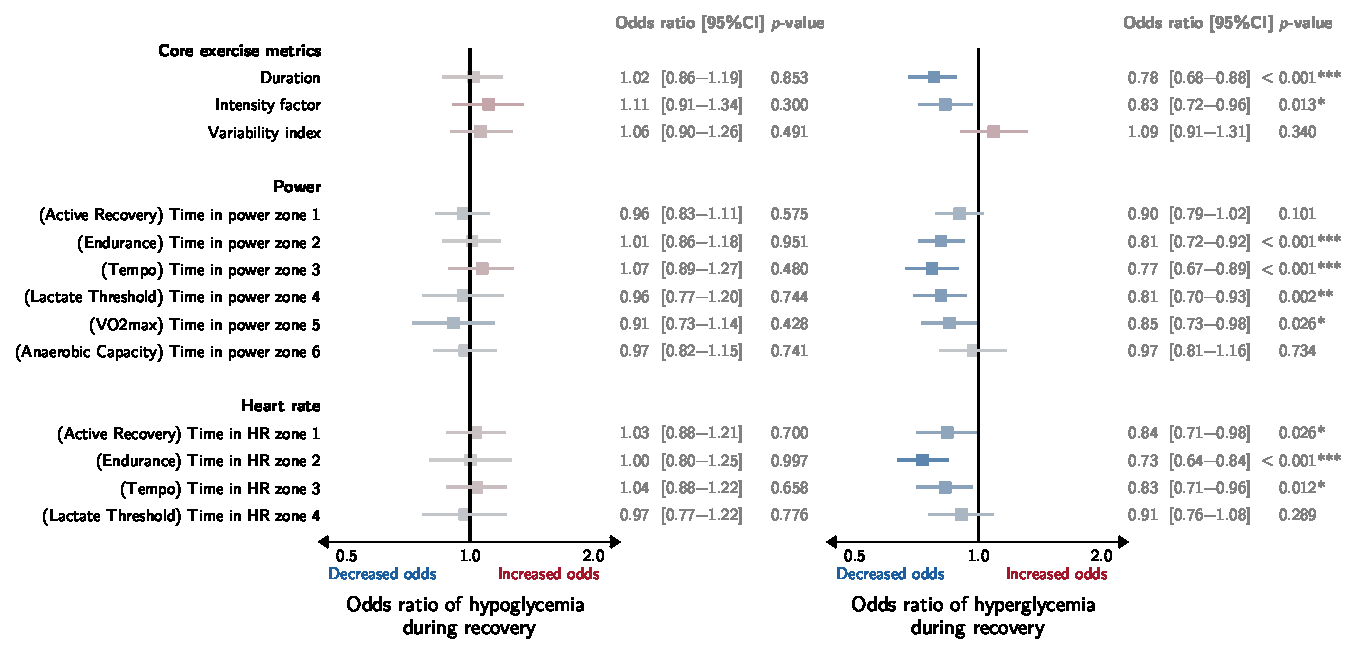
\includegraphics[trim=0cm 0cm 0cm 8mm, clip, width=.95\textwidth]{figure/train/coef_binomial_recovery.pdf}
    \end{subfigure}
    \begin{subfigure}{\textwidth}
        \centering
        \caption{}
        \label{fig:reg-train-sleep}
        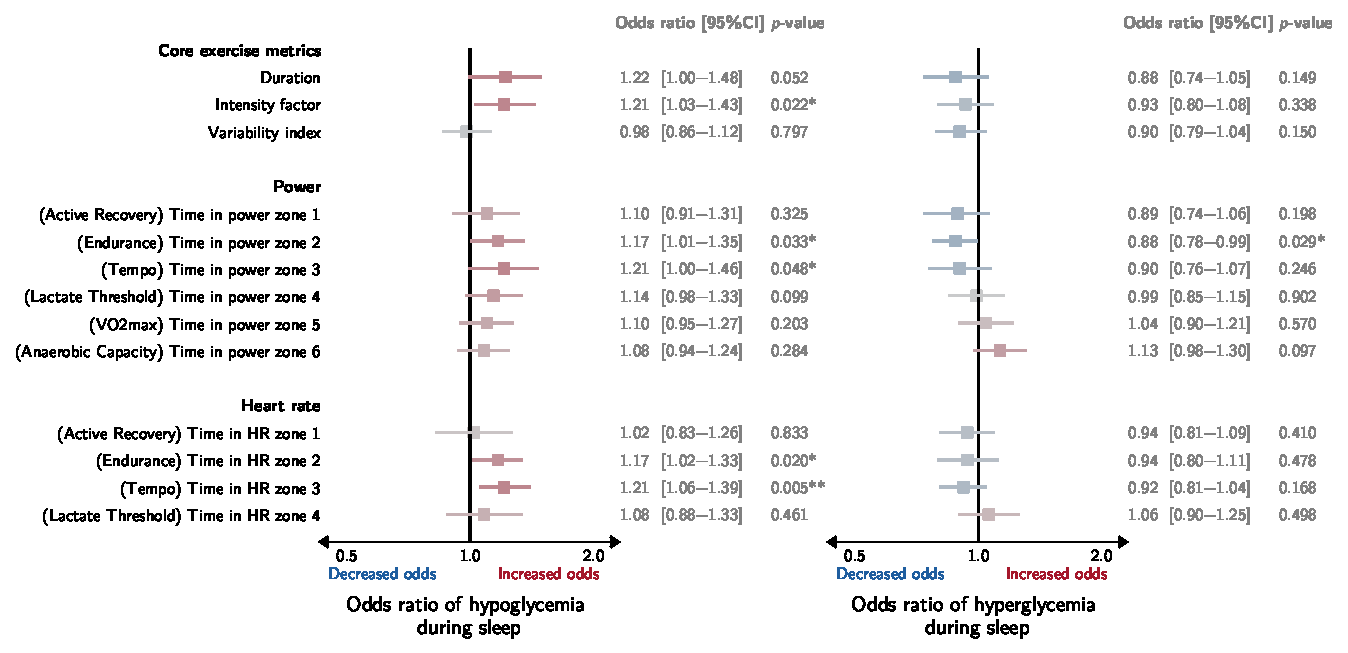
\includegraphics[trim=0cm 0cm 0cm 8mm, clip, width=.95\textwidth]{figure/train/coef_binomial_sleep.pdf}
    \end{subfigure}
\end{figure}

\begin{figure}[hbtp]
    \centering
    \caption[Full results of association analysis on training days]{Full results of association analysis on training days for the odds of \subrefb{fig:reg-train-hypo-full} hypoglycemia and \subrefb{fig:reg-train-hyper-full} hyperglycemia.}
    \label{fig:reg-train-full}
    \begin{subfigure}{\textwidth}
        \centering
        \caption{}
        \label{fig:reg-train-hypo-full}
        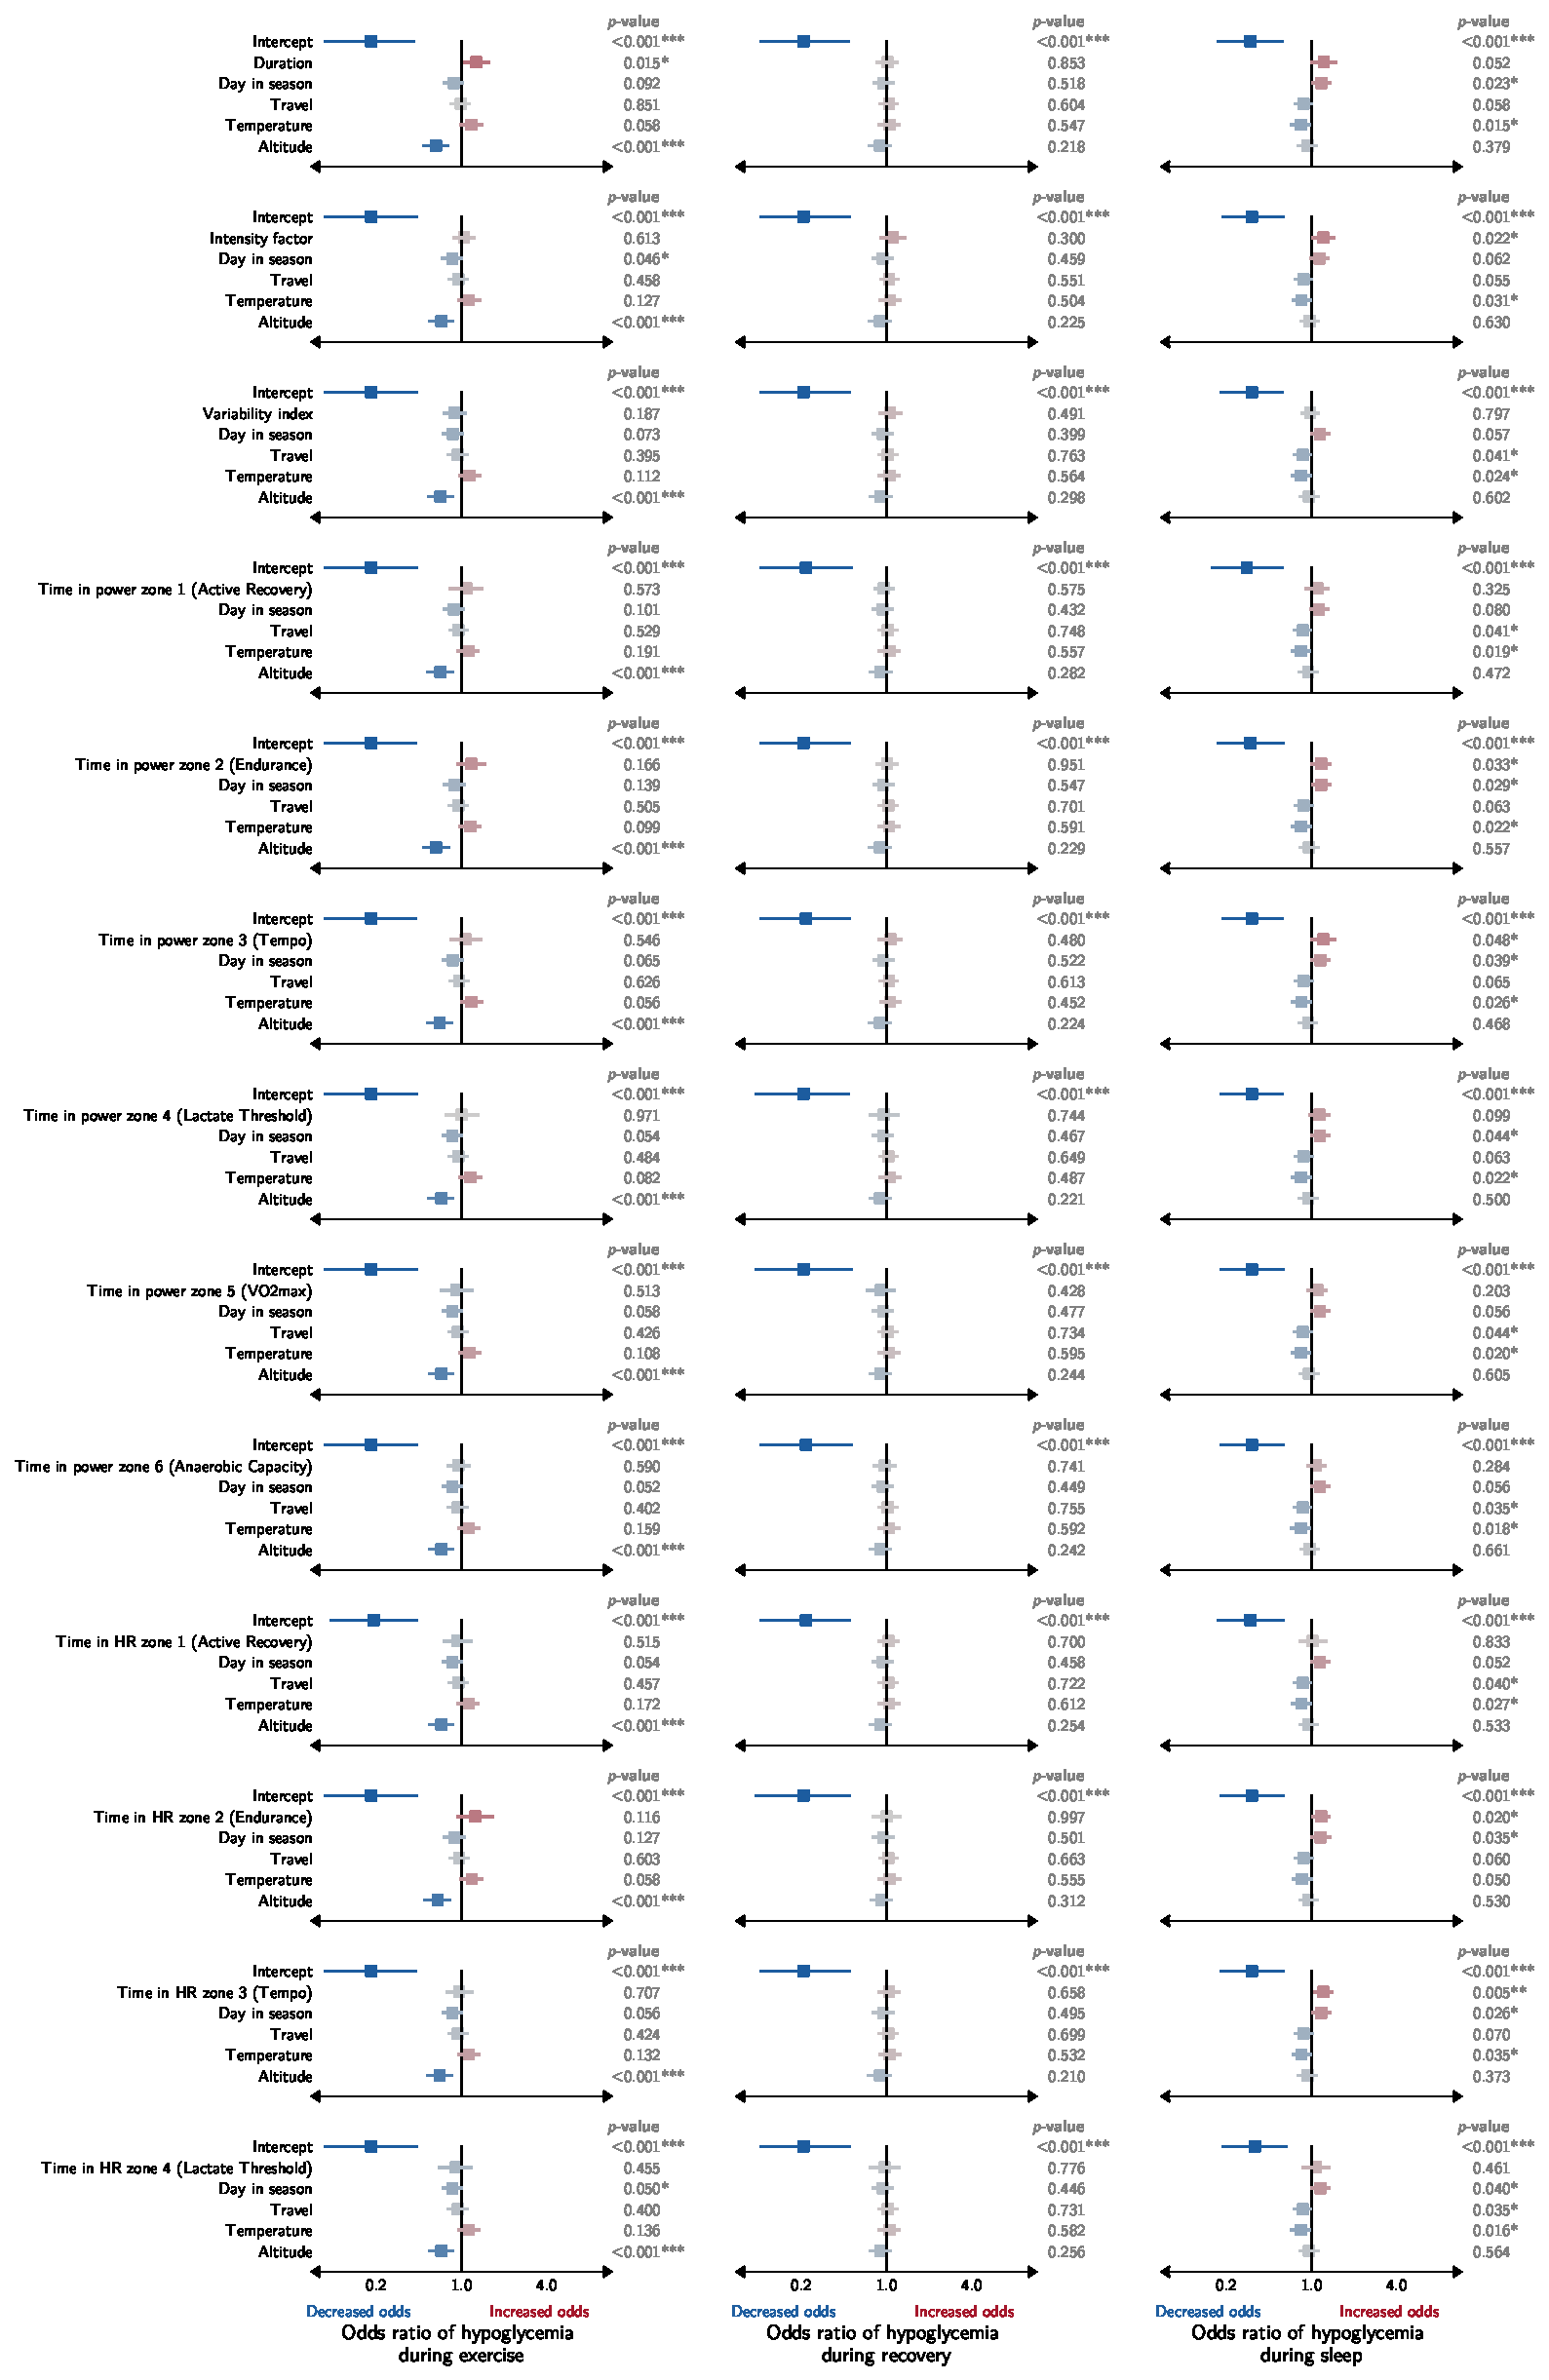
\includegraphics[width=\textwidth]{figure/train/coef_env_train_binomial_hypo.pdf}
    \end{subfigure}
\end{figure}
\begin{figure}[hbtp]\ContinuedFloat
    \begin{subfigure}{\textwidth}
        \centering
        \caption{}
        \label{fig:reg-train-hyper-full}
        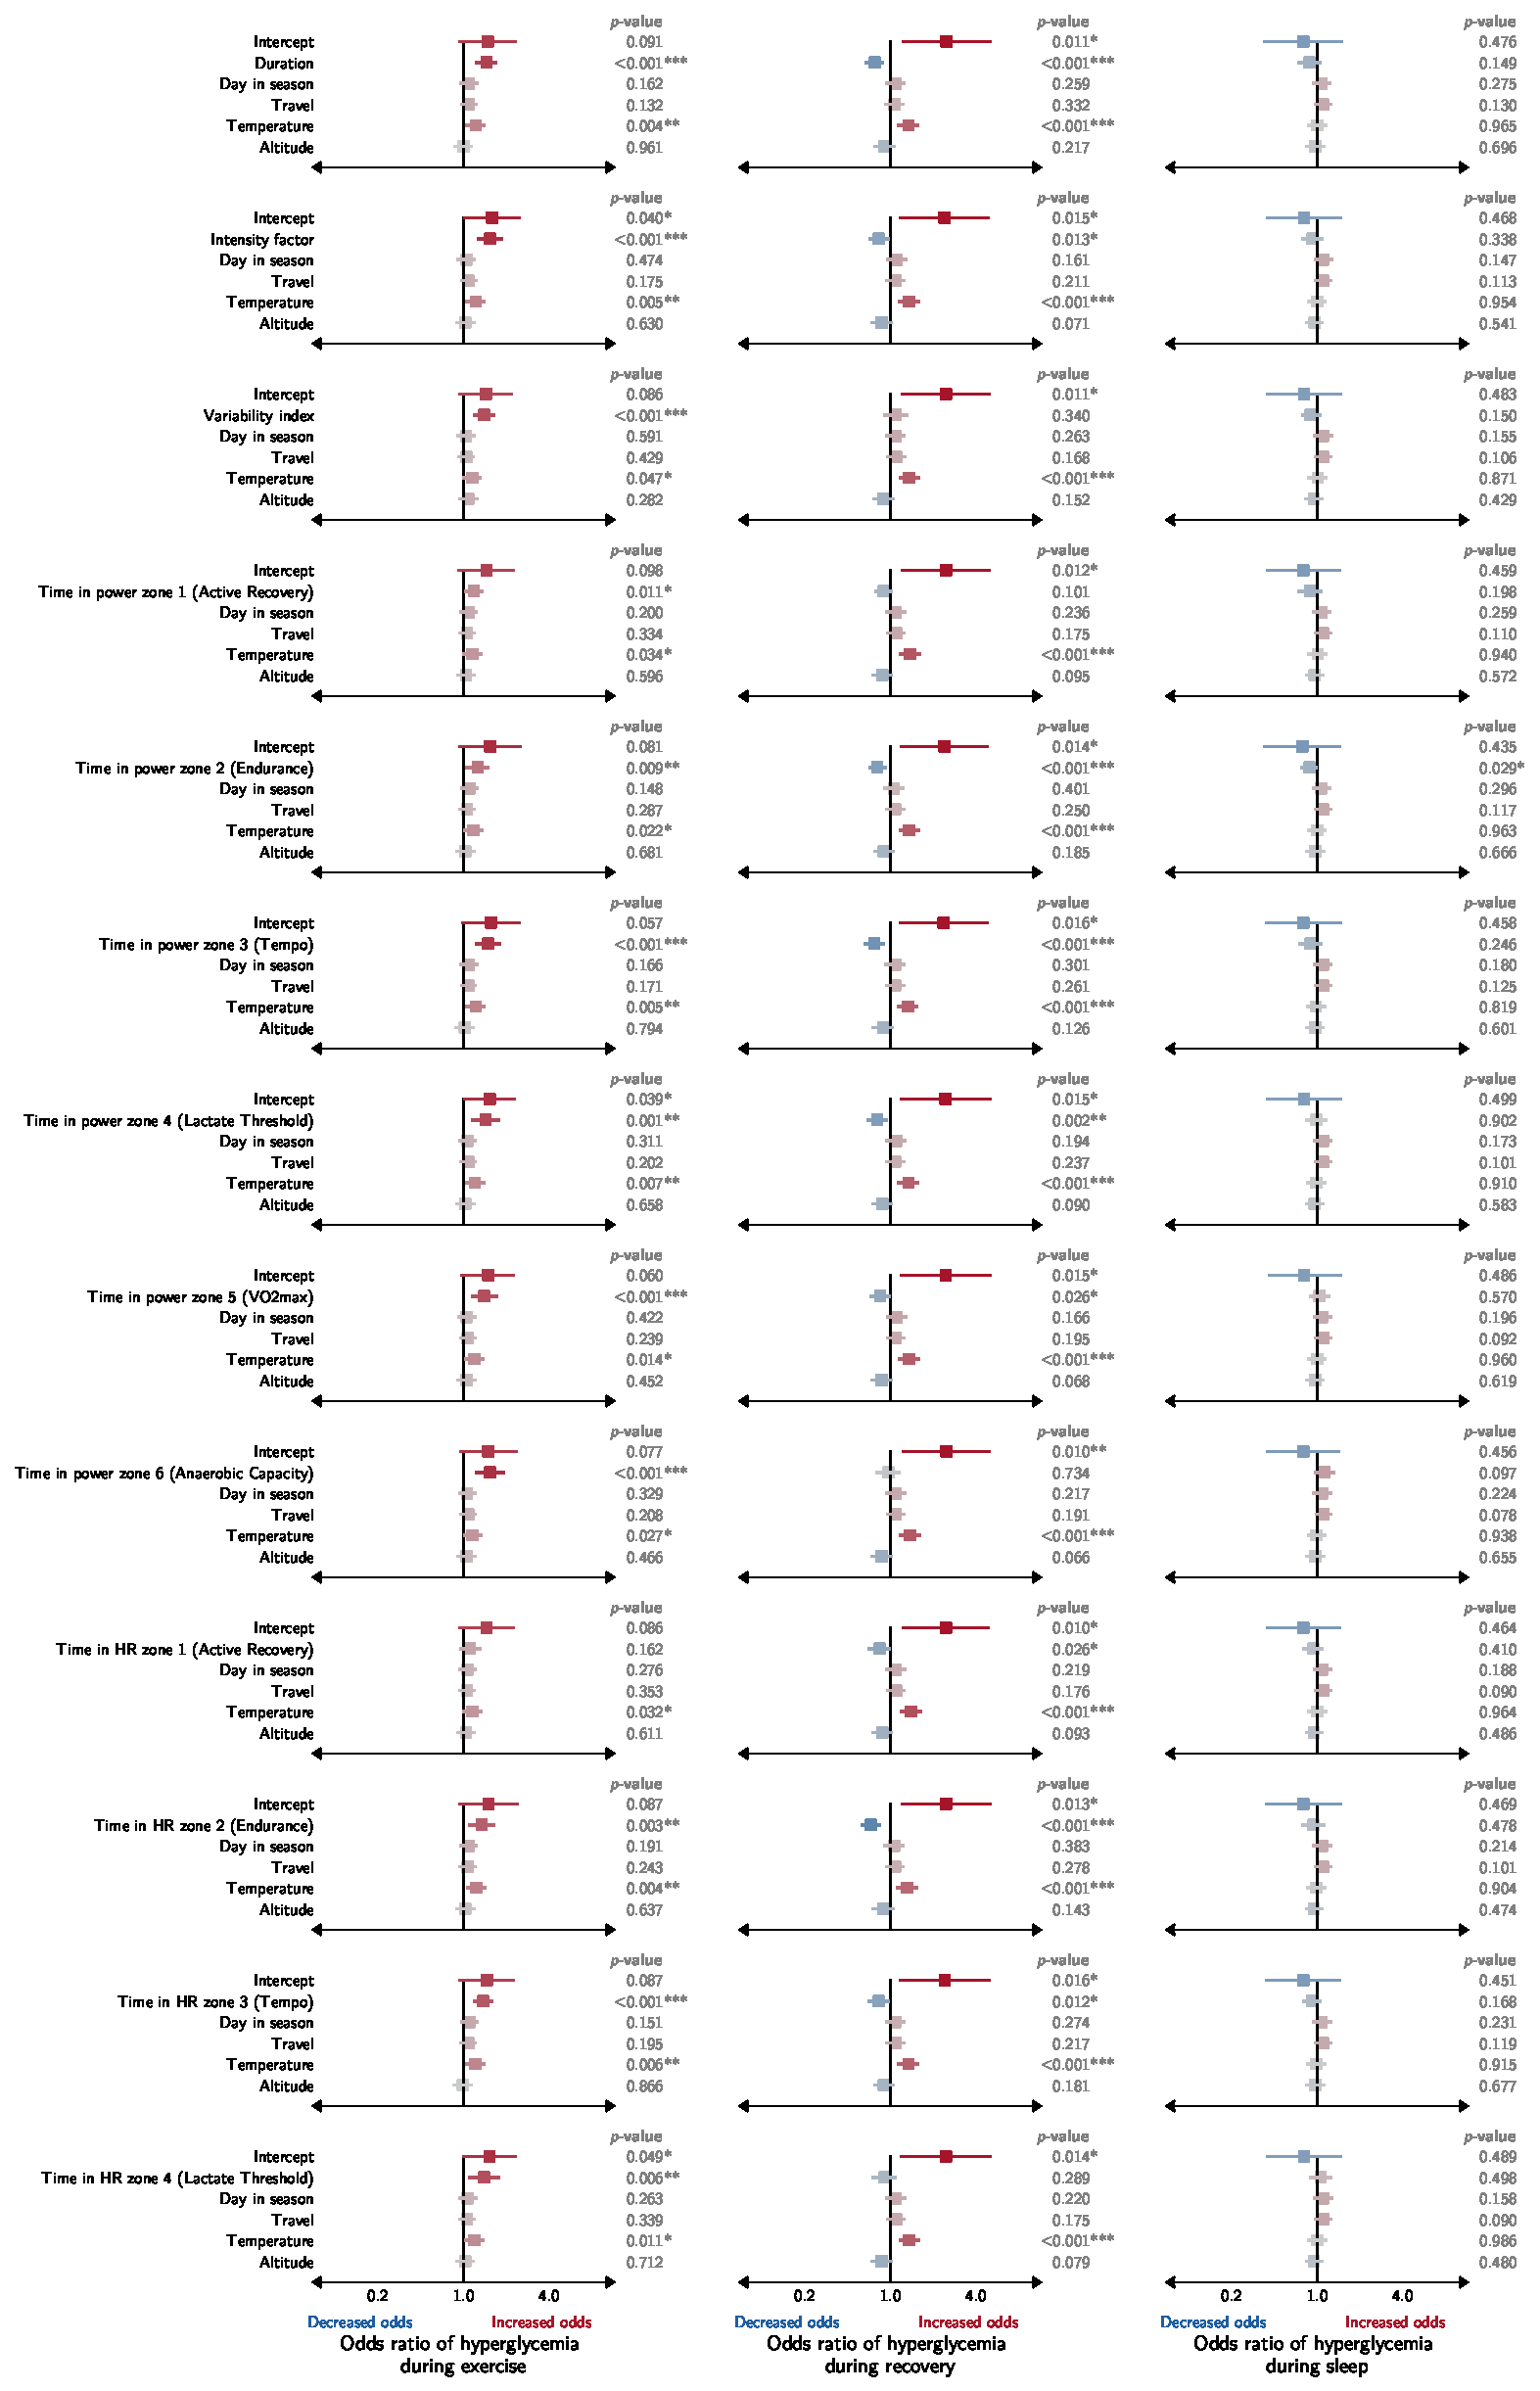
\includegraphics[width=\textwidth]{figure/train/coef_env_train_binomial_hyper.pdf}
    \end{subfigure}
\end{figure}

% ------------------------------ comp

\begin{figure}
    \centering
    \caption[Summary of association analysis on competition days]{Summary of association analysis on competition days for dysglycemia during \subrefb{fig:reg-comp-exercise} exercise, \subrefb{fig:reg-comp-recovery} recovery, and \subrefb{fig:reg-comp-sleep} sleep.}
    \label{fig:reg-comp}
    \begin{subfigure}{\textwidth}
        \centering
        \caption{}
        \label{fig:reg-comp-exercise}
        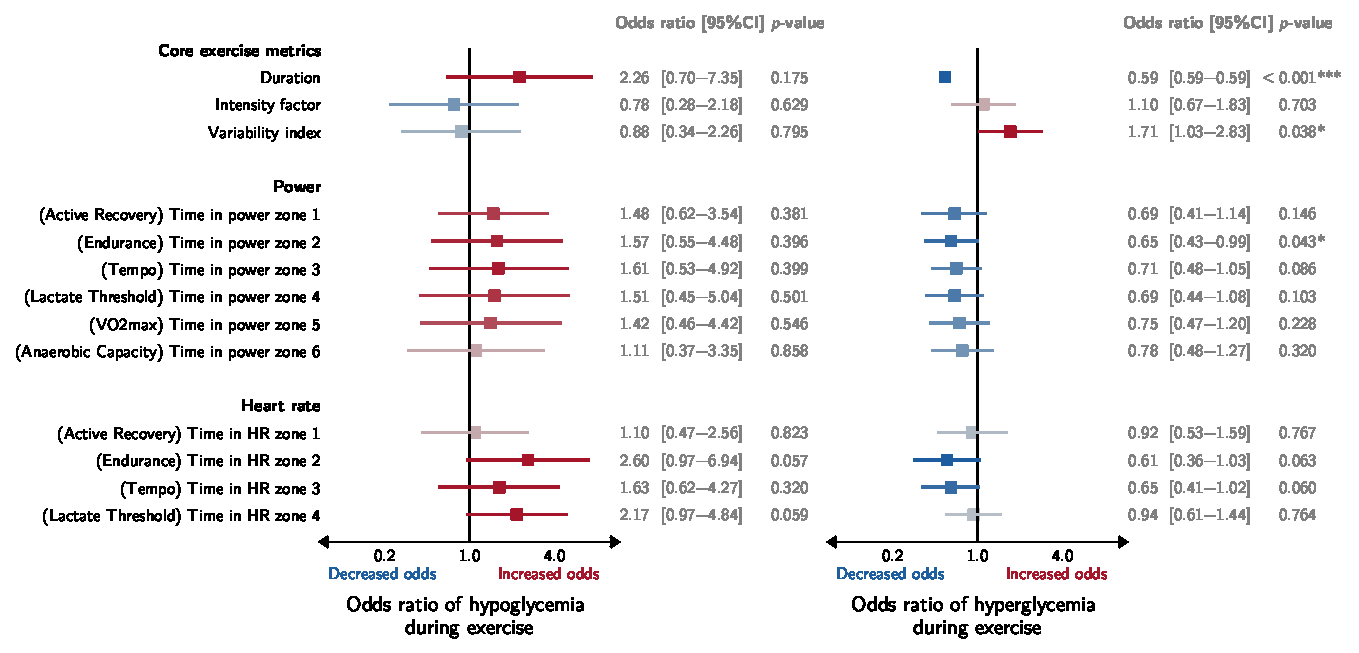
\includegraphics[trim=0cm 0cm 0cm 8mm, clip, width=.95\textwidth]{figure/comp/coef_binomial_exercise.pdf}
    \end{subfigure}
    \begin{subfigure}{\textwidth}
        \centering
        \caption{}
        \label{fig:reg-comp-recovery}
        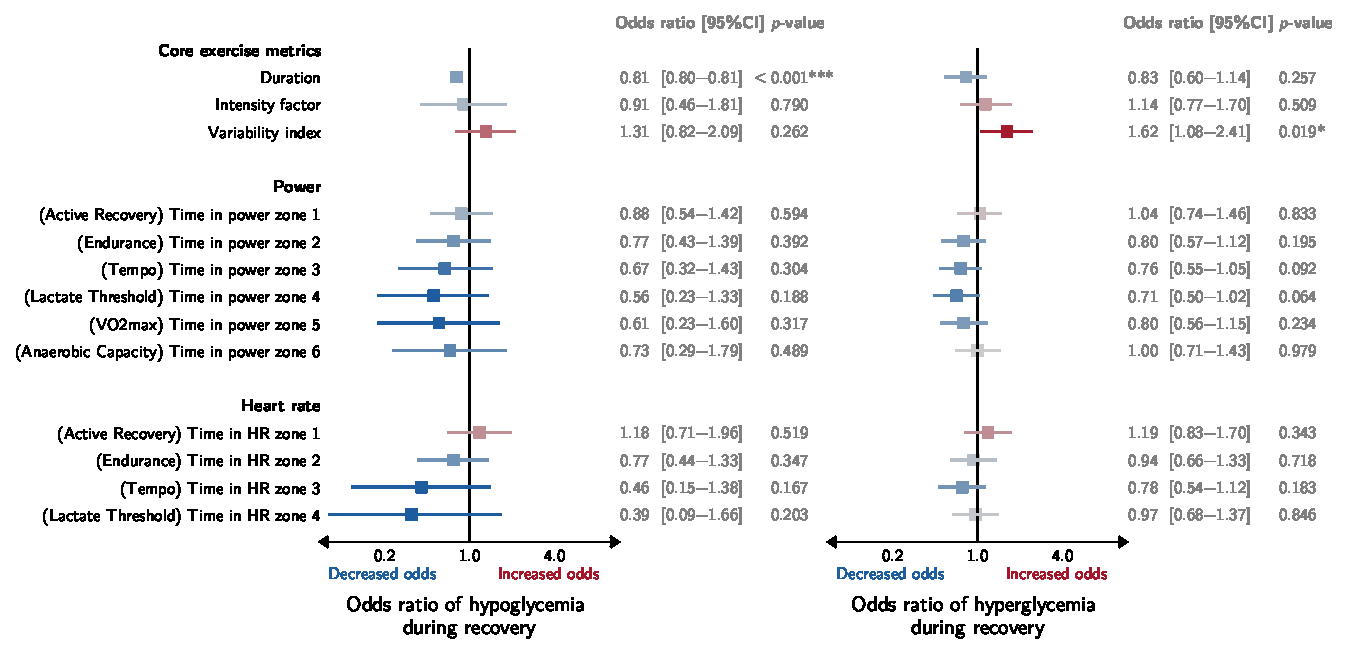
\includegraphics[trim=0cm 0cm 0cm 8mm, clip, width=.95\textwidth]{figure/comp/coef_binomial_recovery.pdf}
    \end{subfigure}
    \begin{subfigure}{\textwidth}
        \centering
        \caption{}
        \label{fig:reg-comp-sleep}
        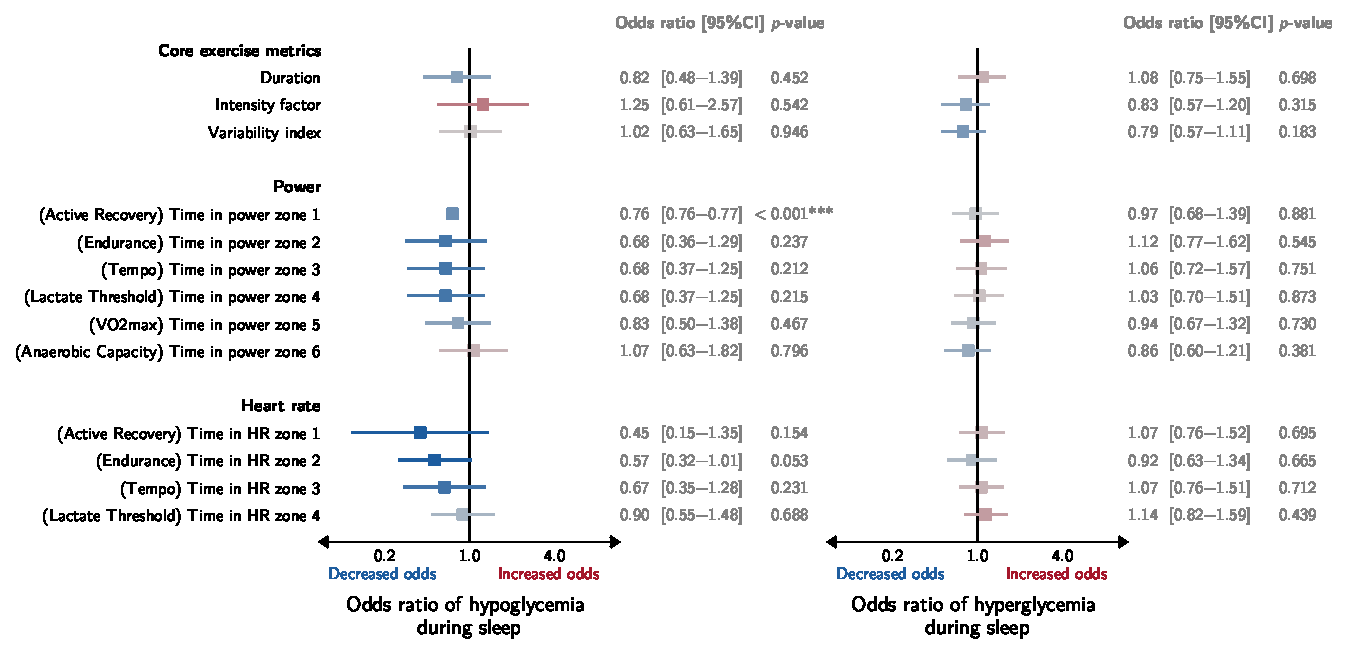
\includegraphics[trim=0cm 0cm 0cm 8mm, clip, width=.95\textwidth]{figure/comp/coef_binomial_sleep.pdf}
    \end{subfigure}
\end{figure}

\begin{figure}[hbtp]
    \centering
    \caption[Full results of association analysis on competition days]{Full results of association analysis on competition days for the odds of \subrefb{fig:reg-comp-hypo-full} hypoglycemia and \subrefb{fig:reg-comp-hyper-full} hyperglycemia.}
    \label{fig:reg-comp-full}
    \begin{subfigure}{\textwidth}
        \centering
        \caption{}
        \label{fig:reg-comp-hypo-full}
        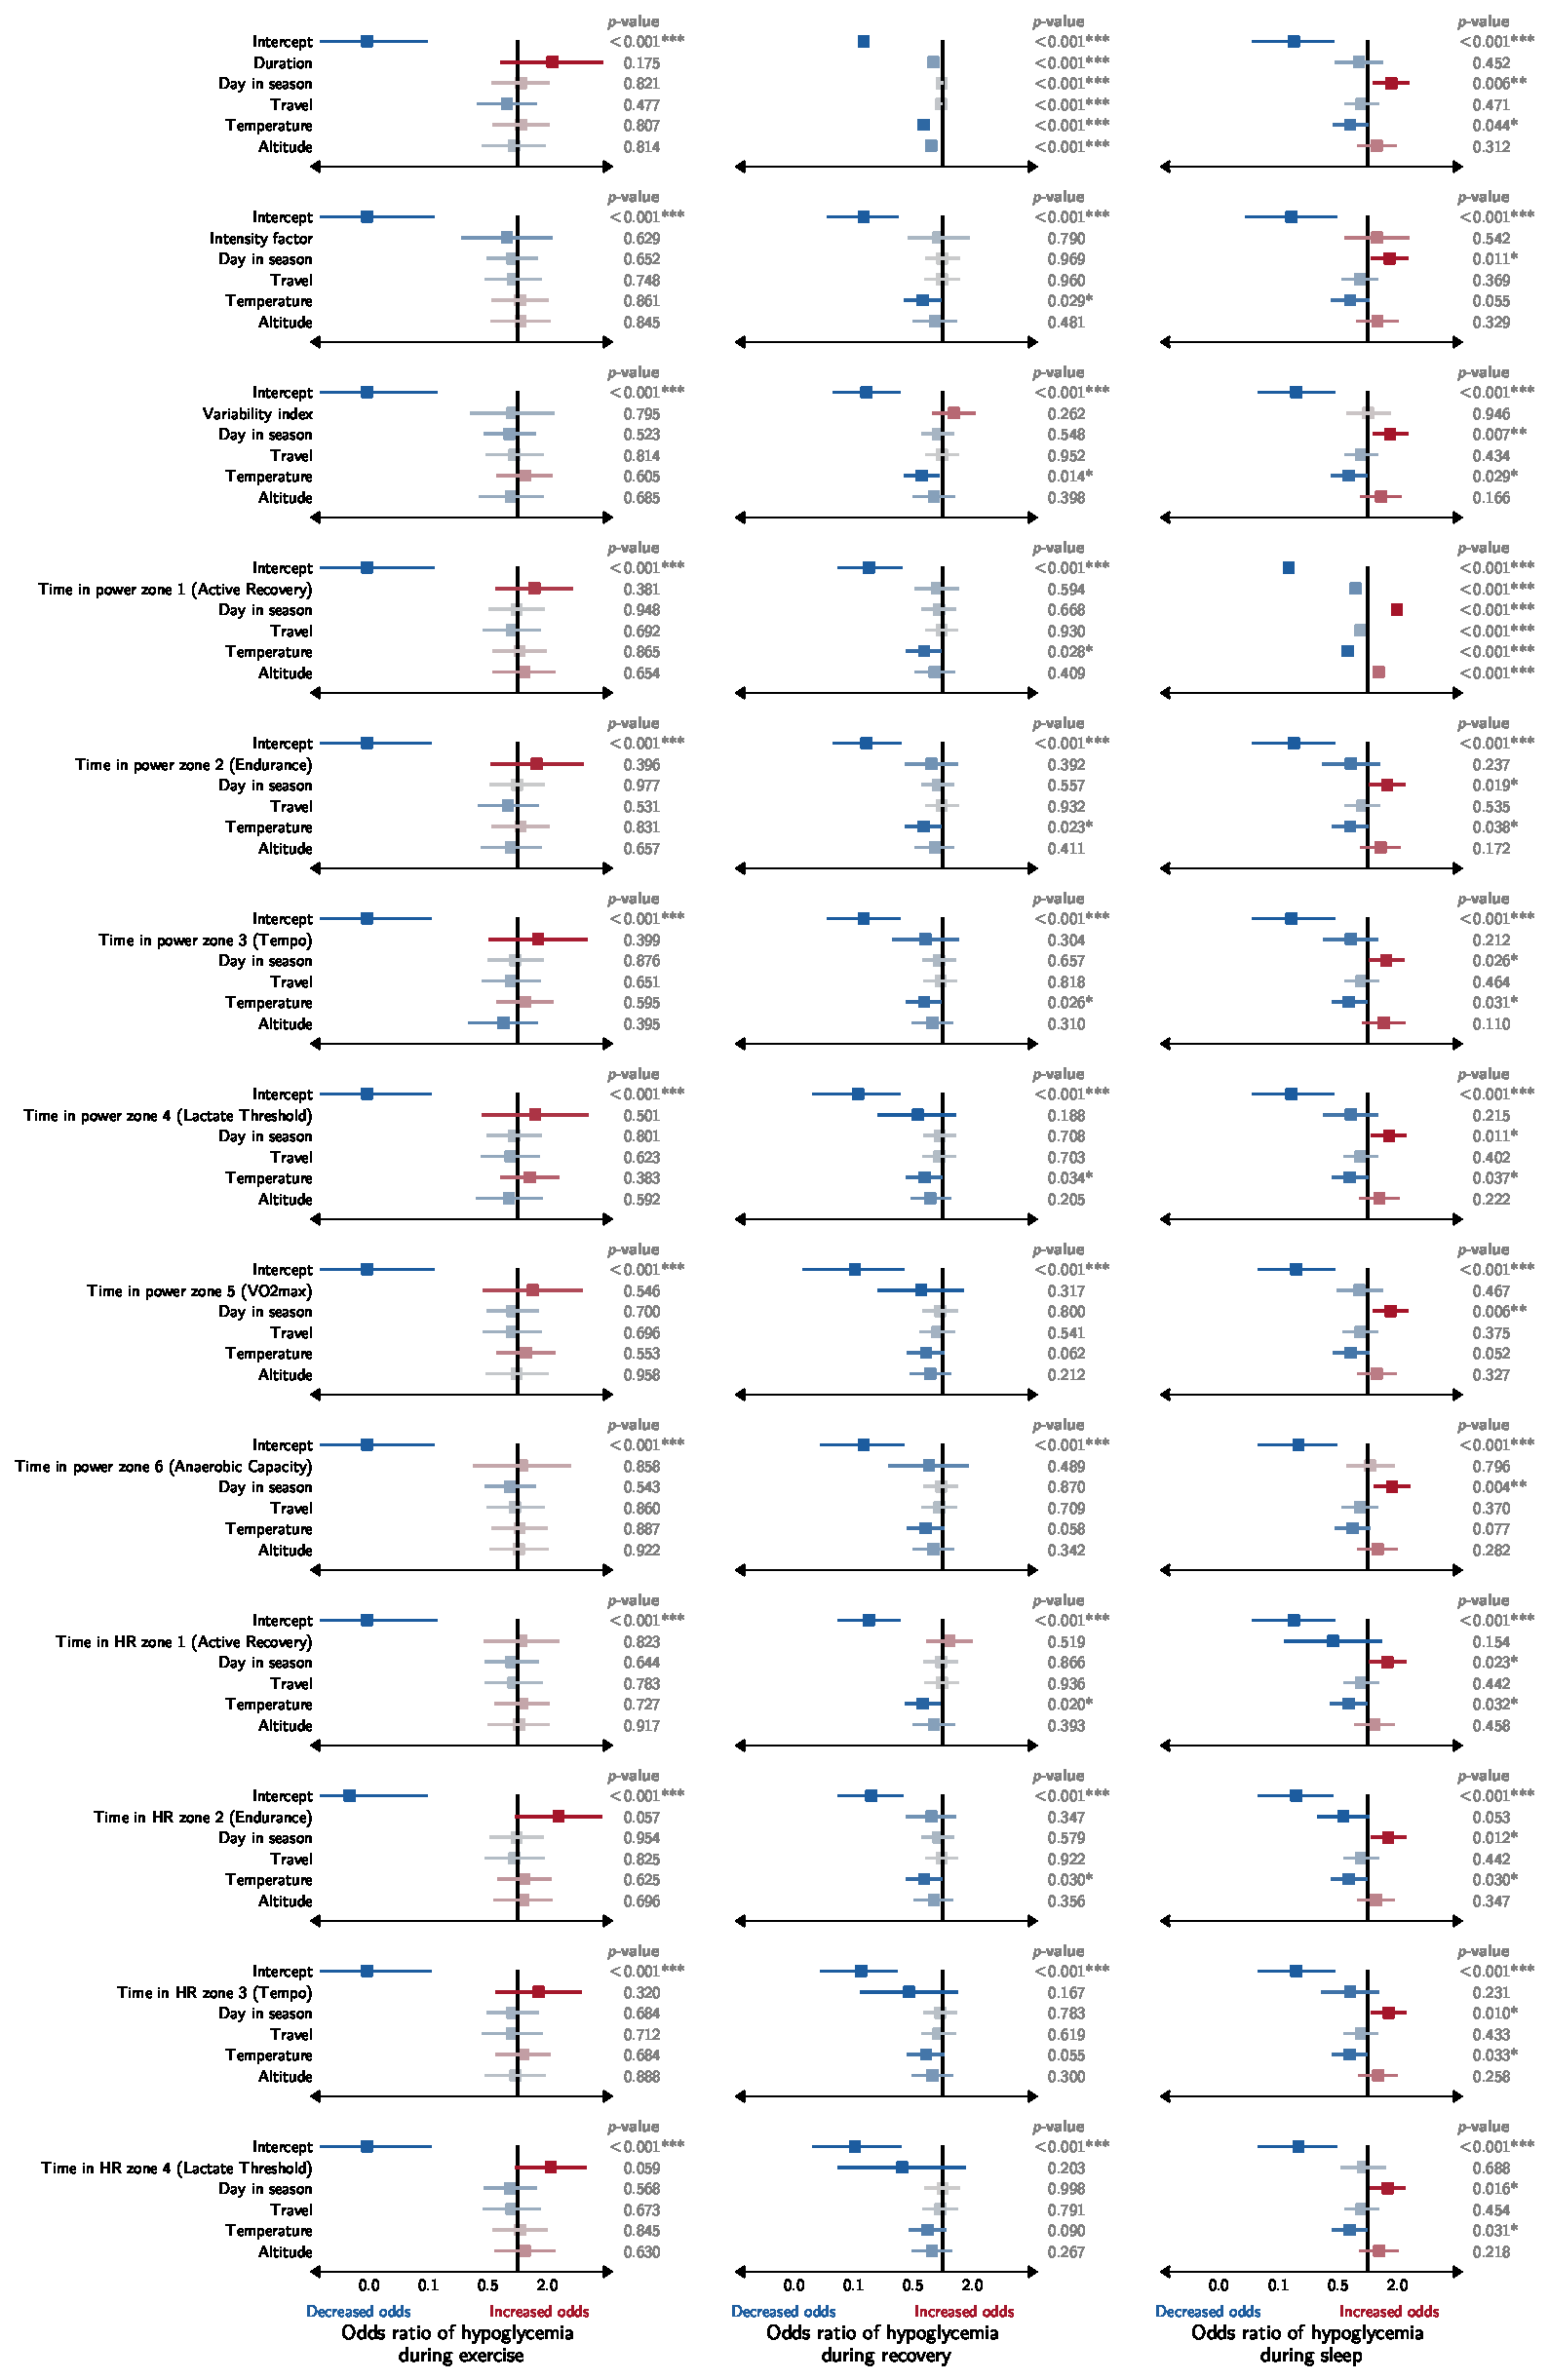
\includegraphics[width=\textwidth]{figure/comp/coef_env_comp_binomial_hypo.pdf}
    \end{subfigure}
\end{figure}
\begin{figure}[hbtp]\ContinuedFloat
    \begin{subfigure}{\textwidth}
        \centering
        \caption{}
        \label{fig:reg-comp-hyper-full}
        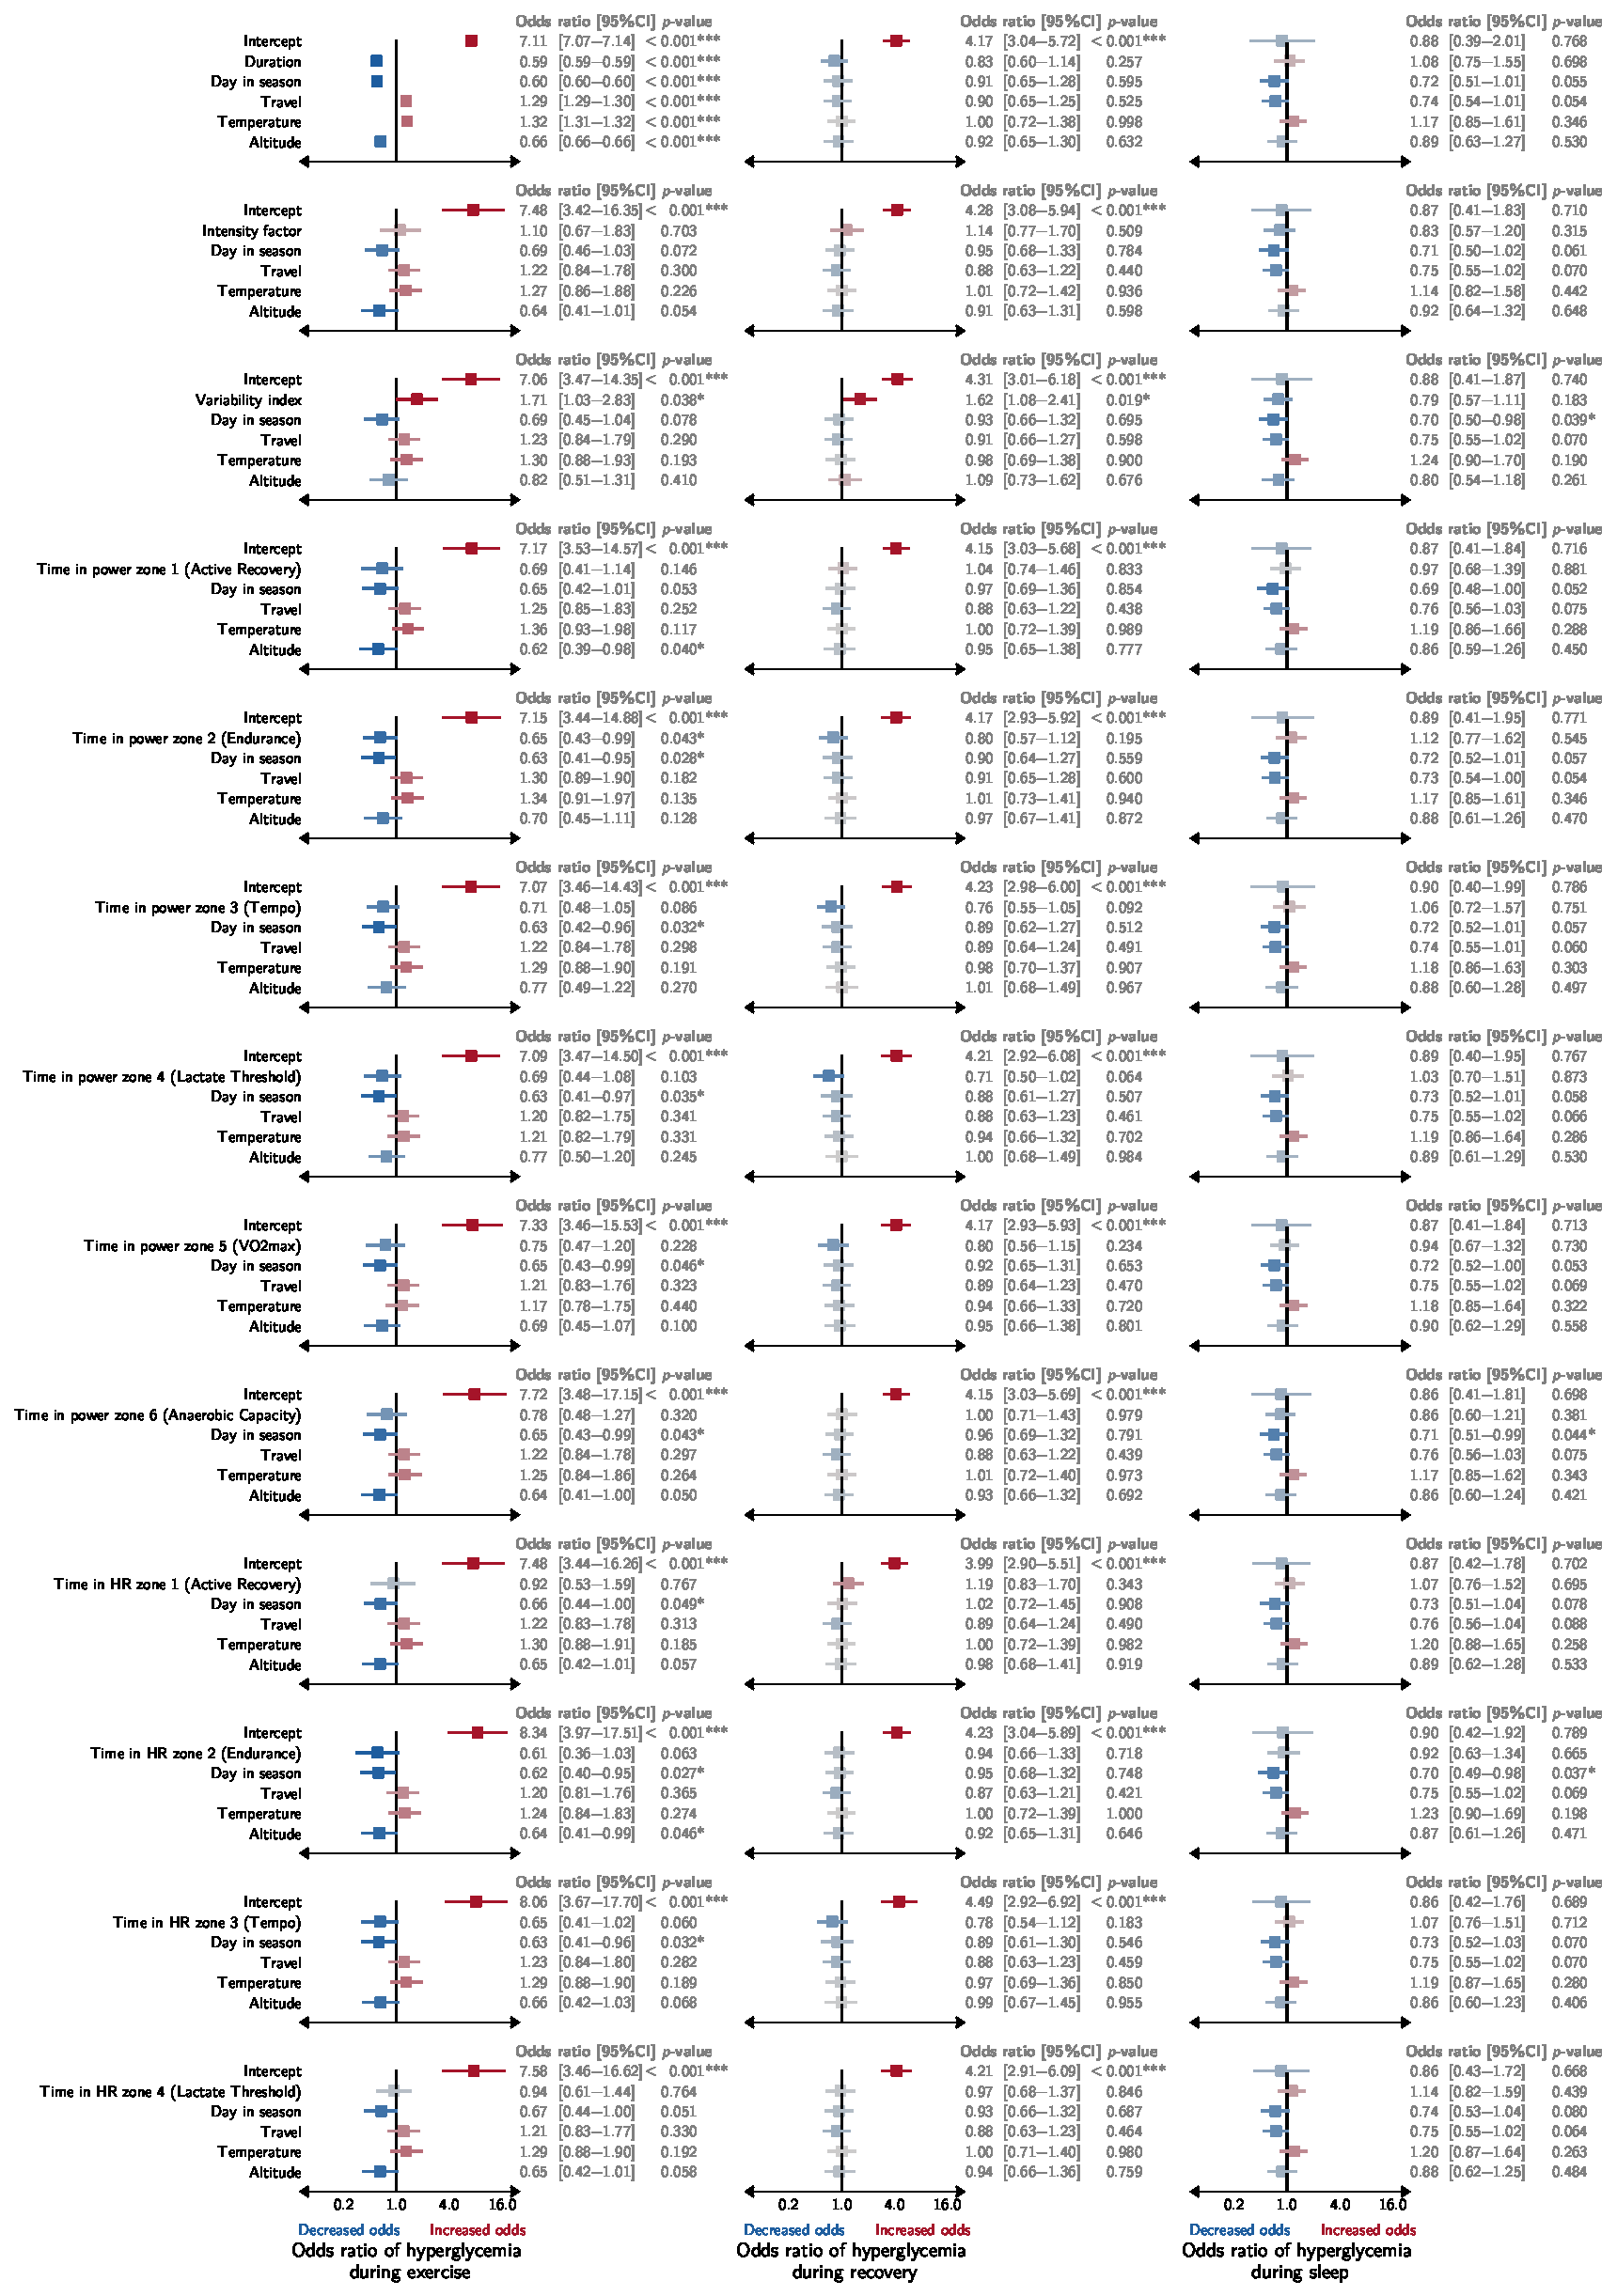
\includegraphics[width=\textwidth]{figure/comp/coef_env_comp_binomial_hyper.pdf}
    \end{subfigure}
\end{figure}

\subsection{Exclusion of participants}
To evaluate the robustness of our model with respect to participants, we performed an analysis where we left individual participants out. In that way, we could evaluate if the participant-specific variation is fully captured by the inclusion of random slopes and intercepts in our model. In particular, we excluded one participant whose data is visibly different from the other participants (participant 9, see Figure~\ref{fig:distributions}). The results of this analysis are shown in Figures~\ref{fig:reg-abl} and \ref{fig:reg-abl-full}. We find that the results of this analysis are largely consistent with those of the main manuscript. 
The associations of the exercise variables of interest with dysglycemia therefore do not seem to be heavily influenced by the data of this participant, and the effect of the individual participant on the dependent variable is likely captured through the inclusion of random effects. 

\begin{figure}
    \centering
    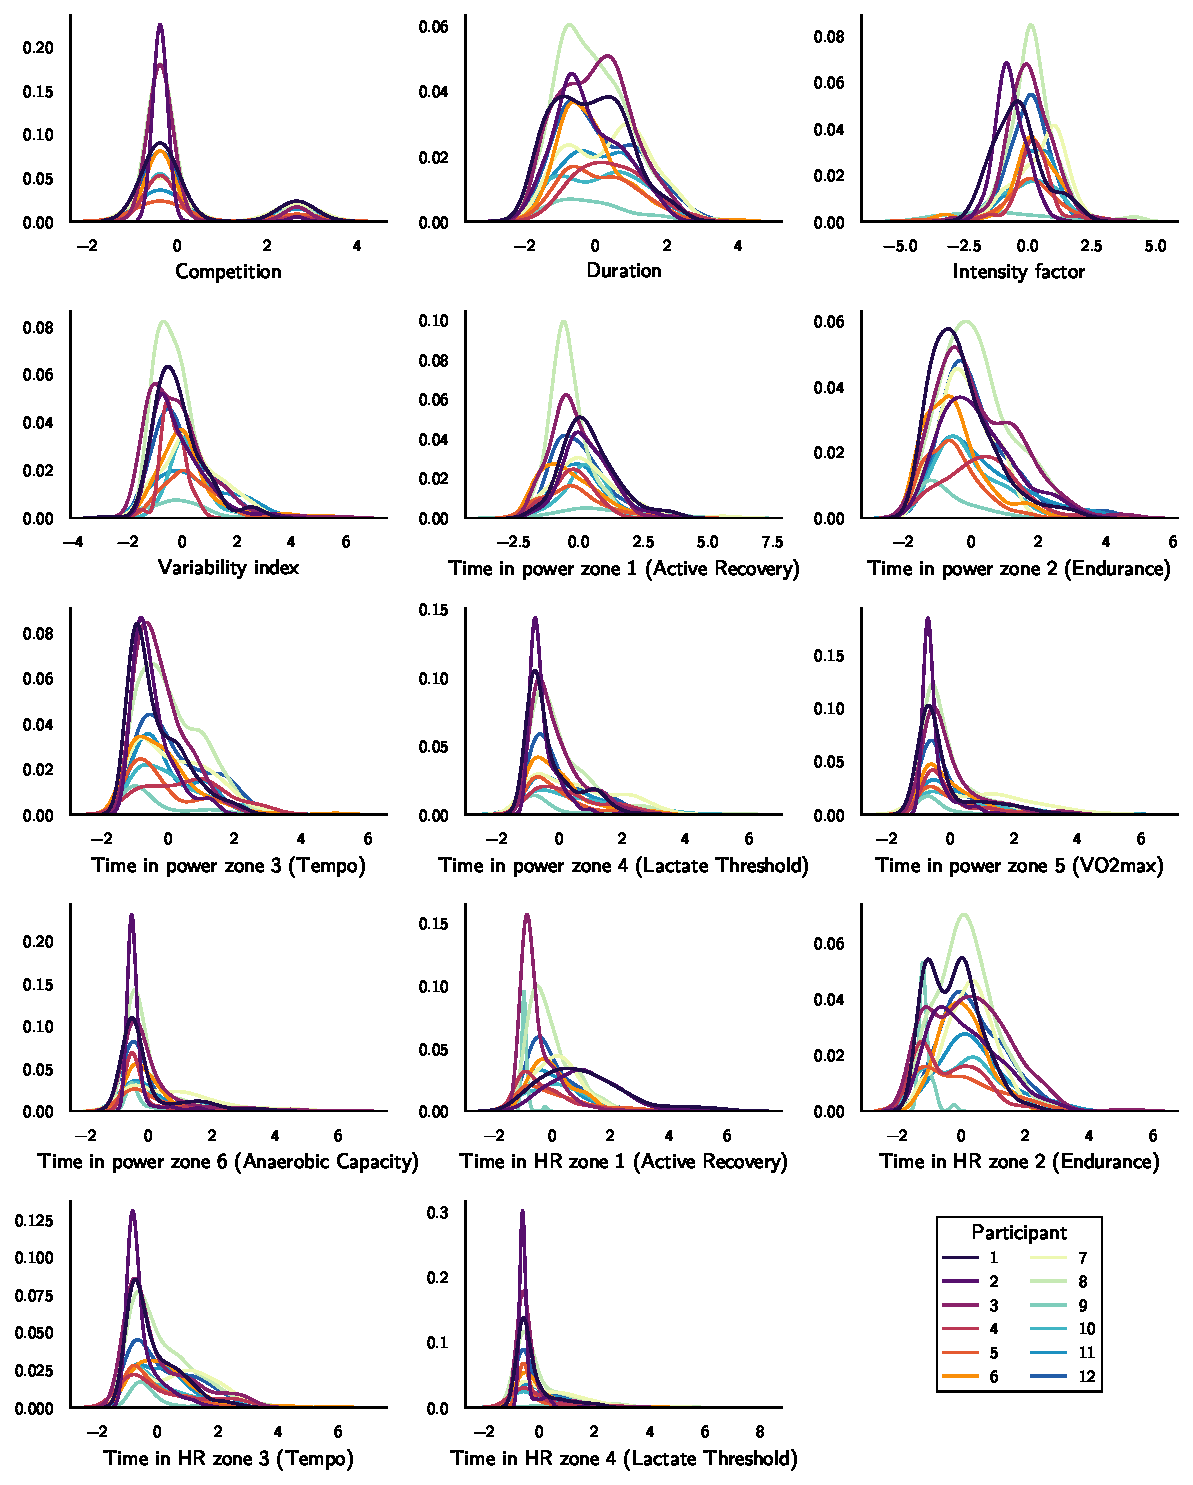
\includegraphics[width=\textwidth]{figure/distributions.pdf}
    \caption{Standardized \gls{kde} distributions of exercise variables by participant}
    \label{fig:distributions}
\end{figure}
% ------------------------------ abl

\begin{figure}
    \centering
    \caption[Summary of association analysis with the exclusion of participants]{Summary of association analysis with the exclusion of participants for dysglycemia during \subrefb{fig:reg-abl-exercise} exercise, \subrefb{fig:reg-abl-recovery} recovery, and \subrefb{fig:reg-abl-sleep} sleep.}
    \label{fig:reg-abl}
    \begin{subfigure}{\textwidth}
        \centering
        \caption{}
        \label{fig:reg-abl-exercise}
        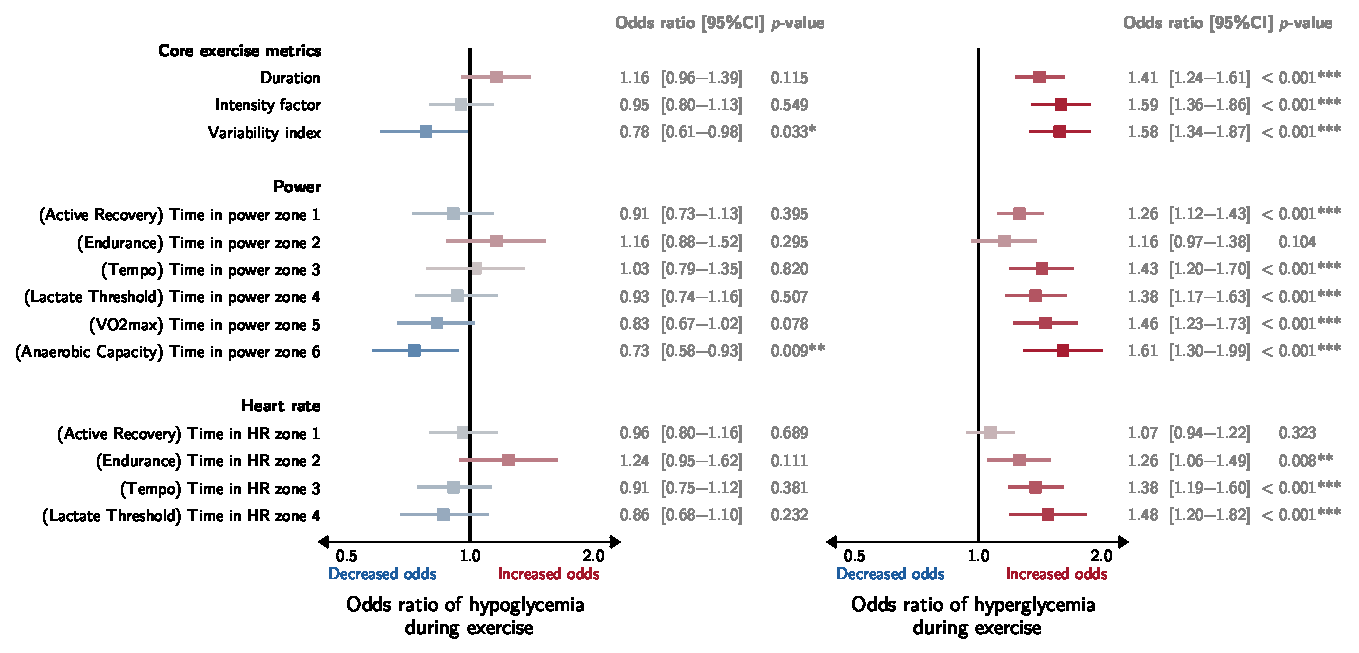
\includegraphics[trim=0cm 0cm 0cm 8mm, clip, width=.95\textwidth]{figure/abl/coef_binomial_exercise.pdf}
    \end{subfigure}
    \begin{subfigure}{\textwidth}
        \centering
        \caption{}
        \label{fig:reg-abl-recovery}
        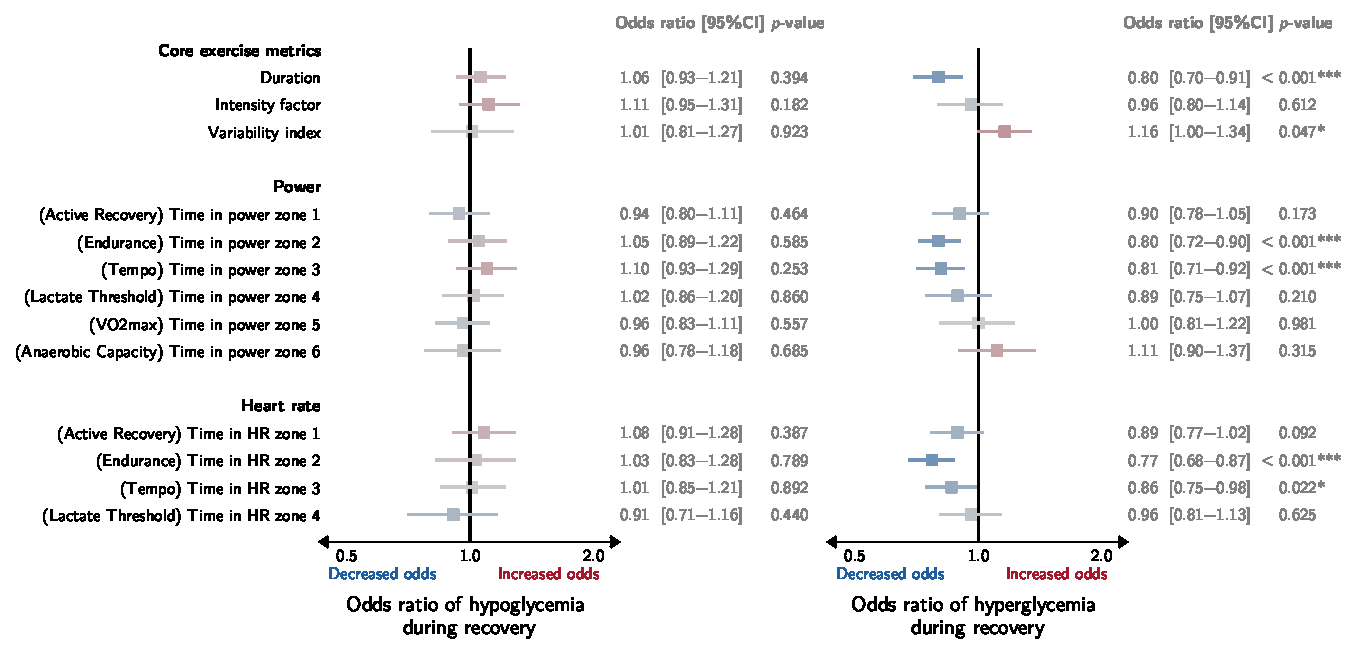
\includegraphics[trim=0cm 0cm 0cm 8mm, clip, width=.95\textwidth]{figure/abl/coef_binomial_recovery.pdf}
    \end{subfigure}
    \begin{subfigure}{\textwidth}
        \centering
        \caption{}
        \label{fig:reg-abl-sleep}
        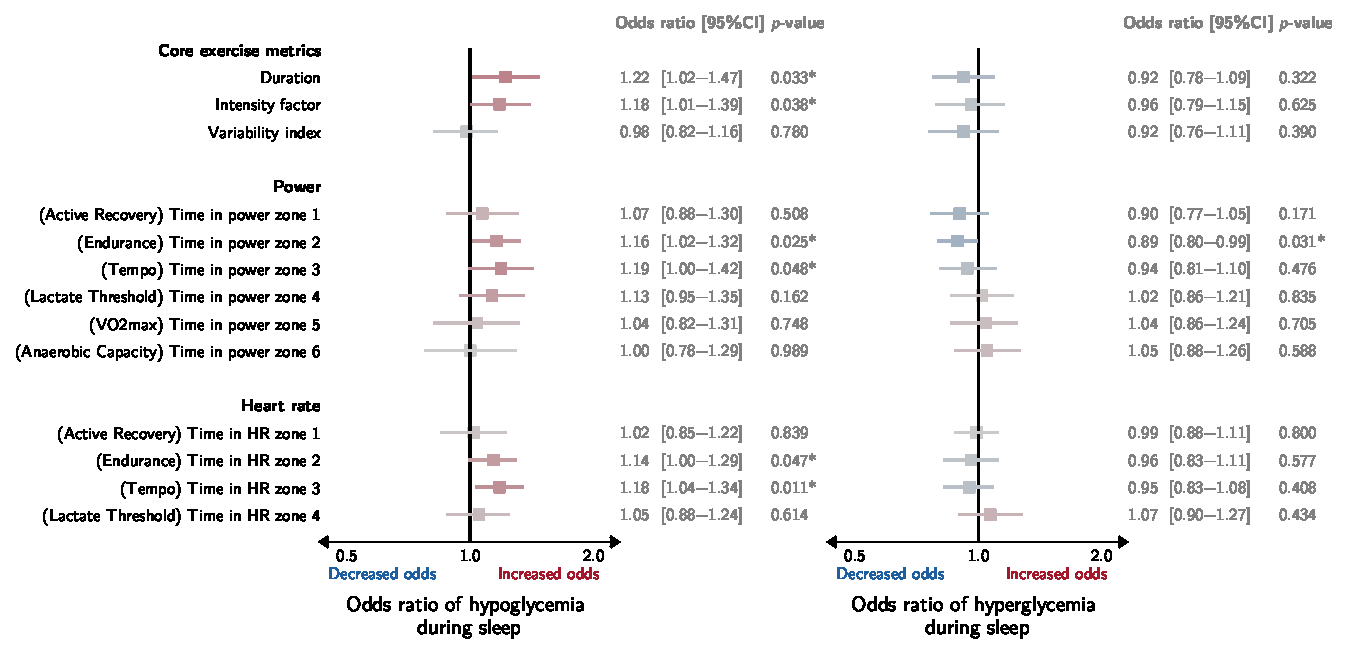
\includegraphics[trim=0cm 0cm 0cm 8mm, clip, width=.95\textwidth]{figure/abl/coef_binomial_sleep.pdf}
    \end{subfigure}
\end{figure}

\begin{figure}[hbtp]
    \centering
    \caption[Full results of association analysis with exclusion of participants]{Full results of association analysis with exclusion of participants for the odds of \subrefb{fig:reg-abl-hypo-full} hypoglycemia and \subrefb{fig:reg-abl-hyper-full} hyperglycemia.}
    \label{fig:reg-abl-full}
    \begin{subfigure}{\textwidth}
        \centering
        \caption[singlelinecheck=off]{}
        \label{fig:reg-abl-hypo-full}
        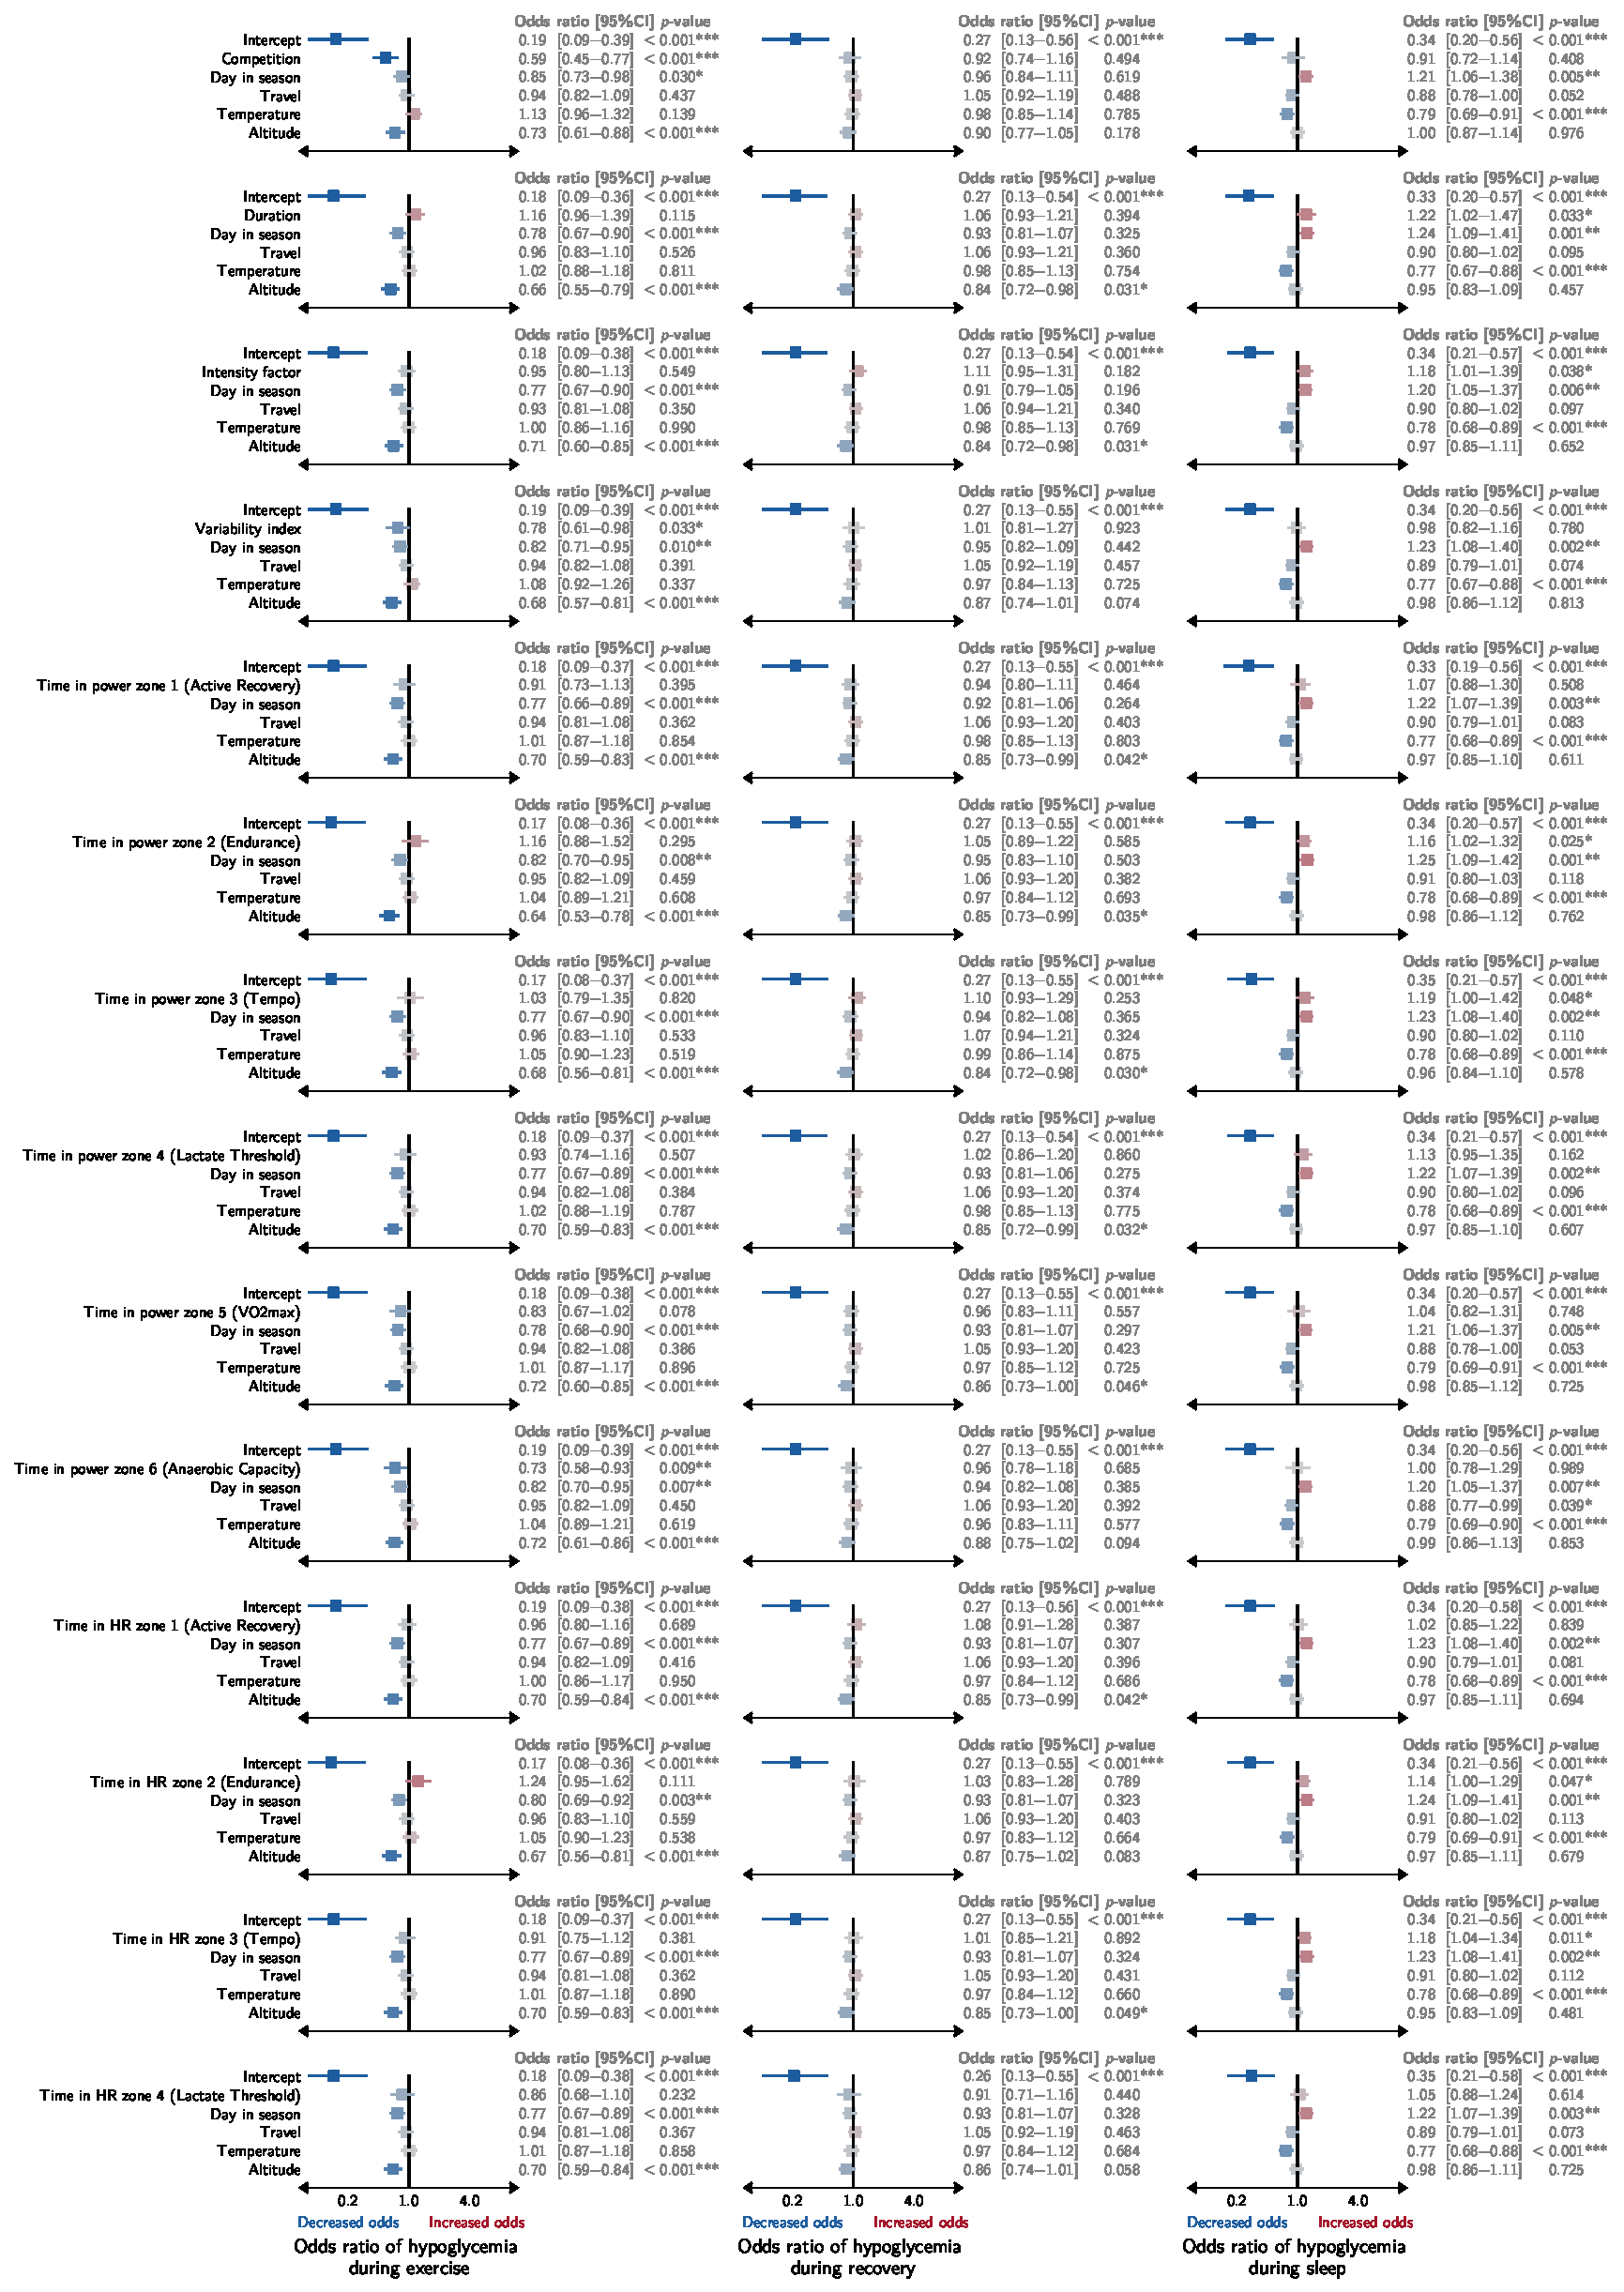
\includegraphics[width=\textwidth]{figure/abl/coef_env_abl_binomial_hypo.pdf}
    \end{subfigure}
\end{figure}
\begin{figure}[hbtp]\ContinuedFloat
    \begin{subfigure}{\textwidth}
        \centering
        \caption{}
        \label{fig:reg-abl-hyper-full}
        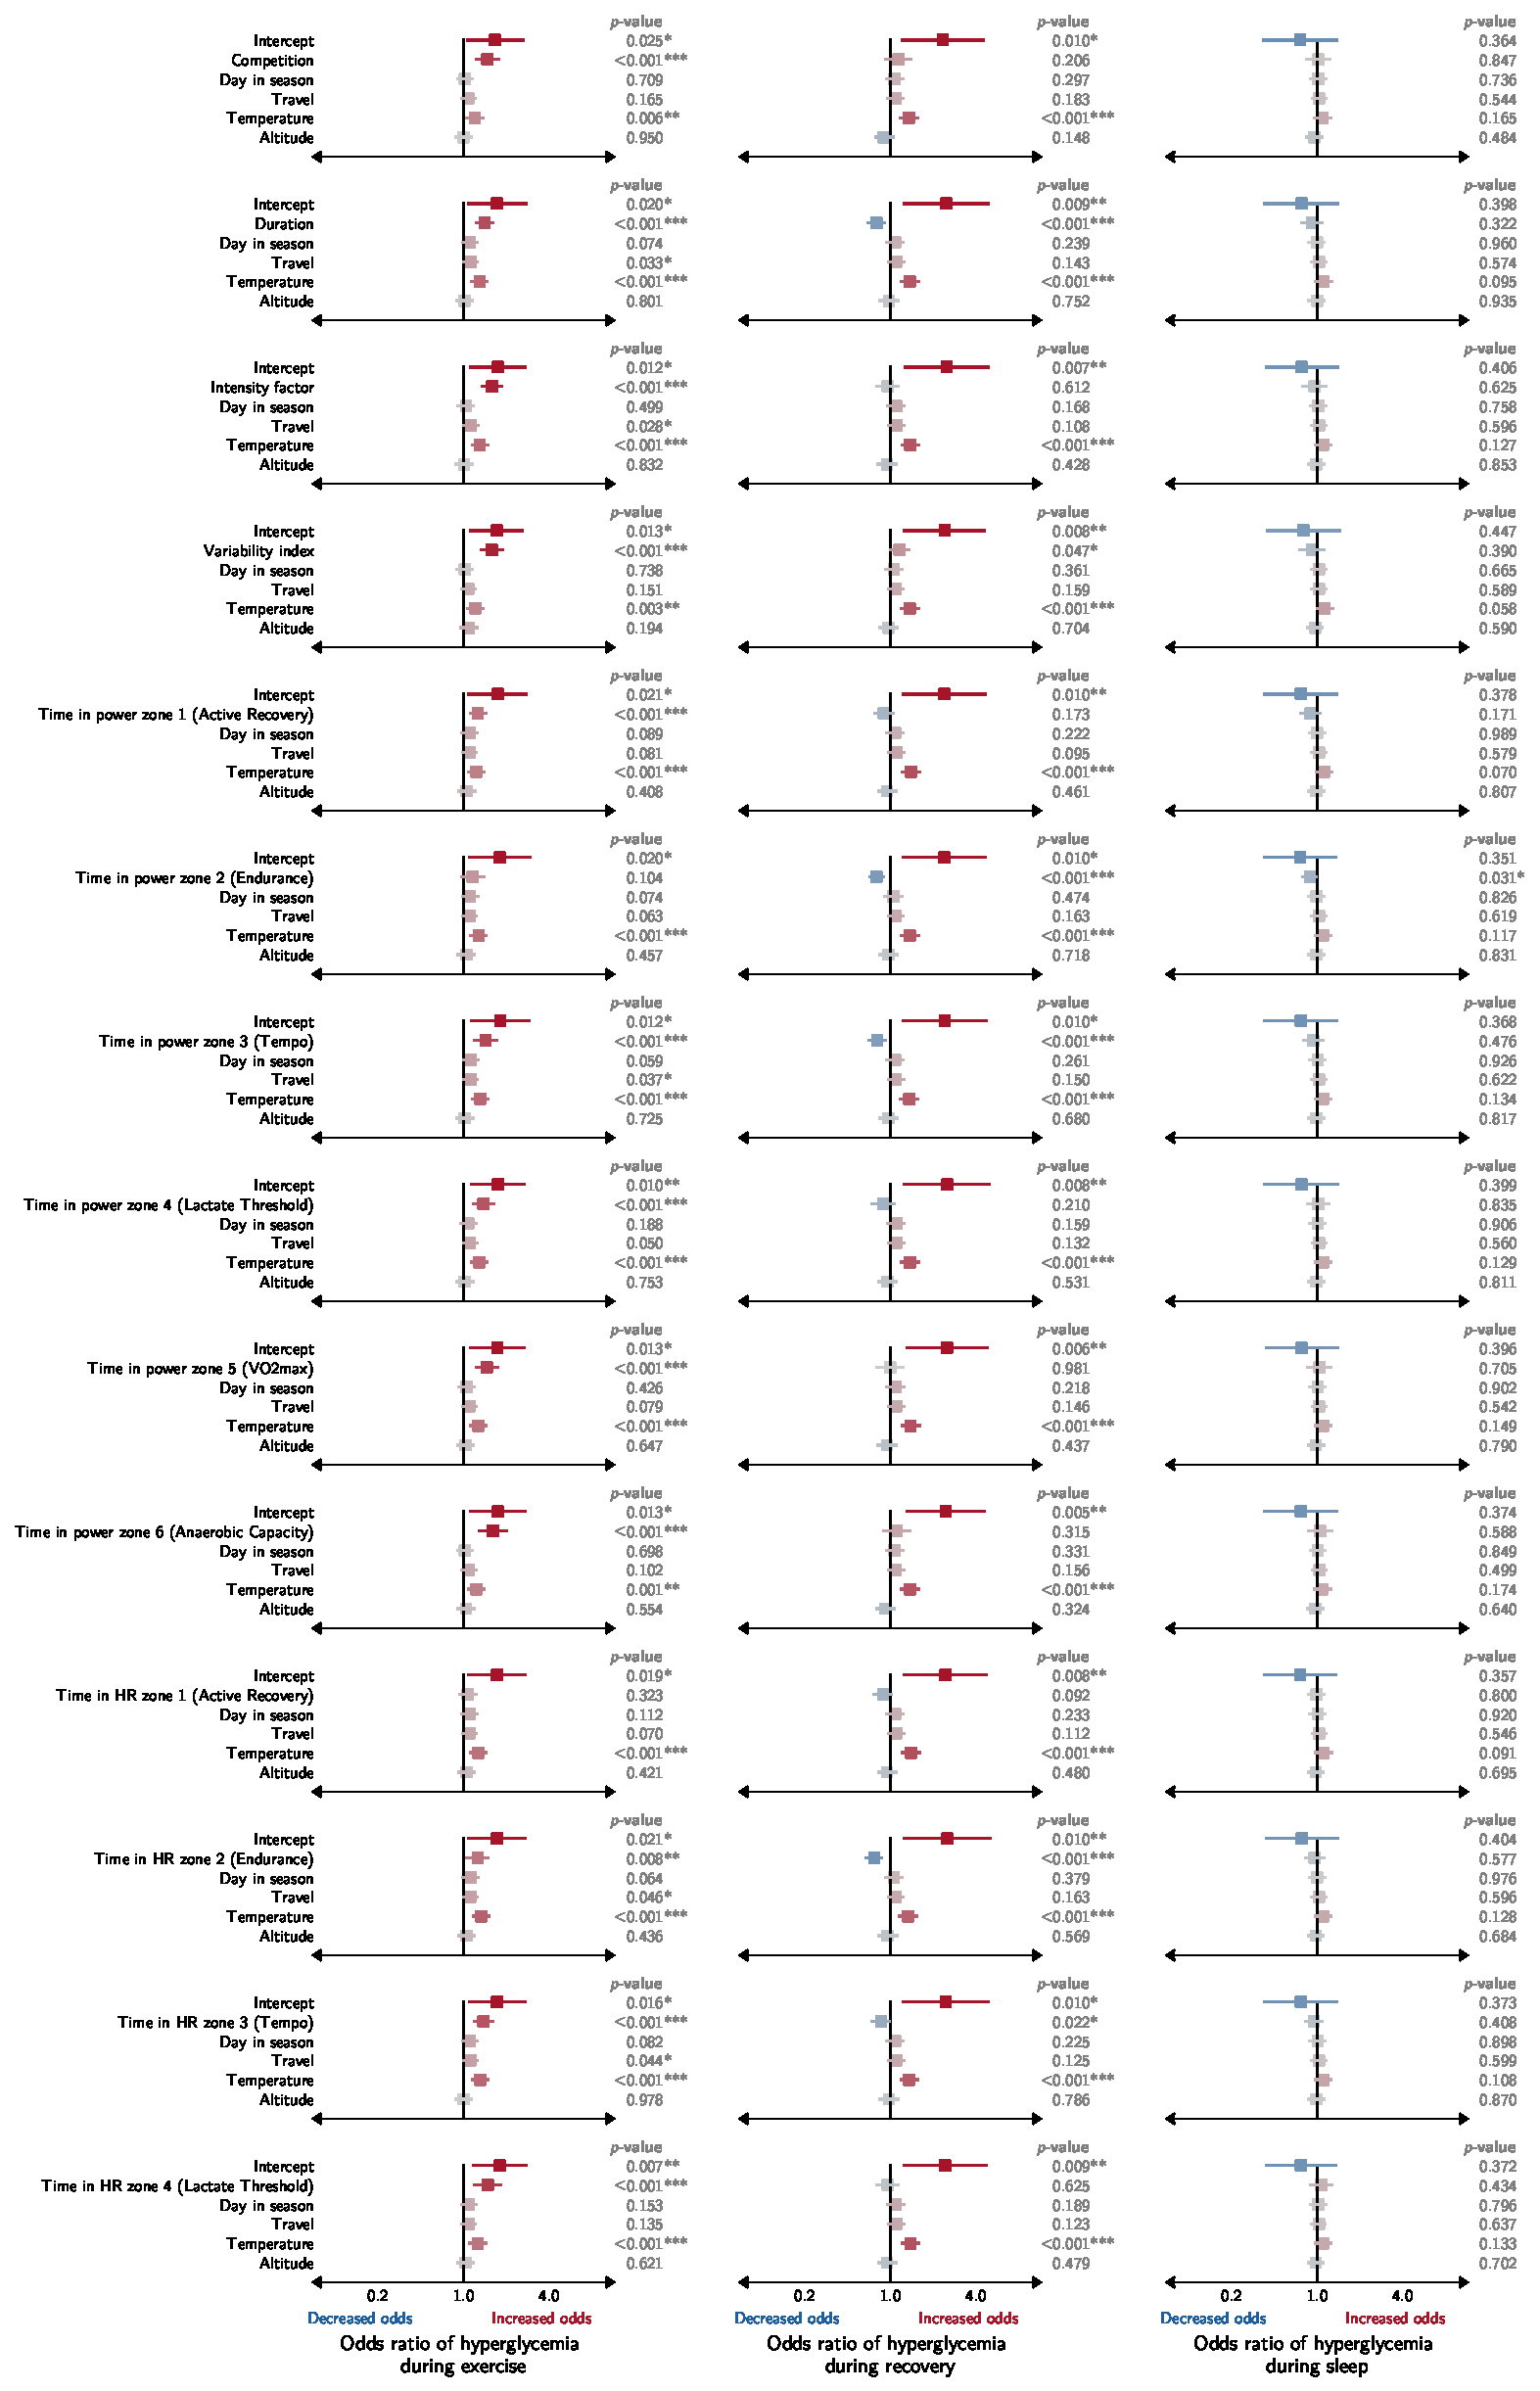
\includegraphics[width=\textwidth]{figure/abl/coef_env_abl_binomial_hyper.pdf}
    \end{subfigure}
\end{figure}

\newpage
\bibliographystyle{apalike}
\bibliography{references.bib}

\end{document}